% Root File for a UC Dissertation / Thesis
% UCD thesis class: c/o Shwaine <shwaine@shwaine.com>
%
% modified by Dylan Beaudette, 2006,2010
% modified  and source uploaded to github by Alex Mandel, 2014
% Source code available at http://github.com/wildintellect/ucdthesis
% \documentclass[11pt]{ucdthesis}
%\documentclass[10pt,twoside,final]{ucdthesis}
% \documentclass[10pt,twoside,draft]{ucdthesis}
% \documentclass[10pt,oneside,final]{ucdthesis}

% TODO: this makes strange things happen in the header...
% this is the version that grad studies wants
\documentclass[11pt,oneside,draft]{ucdthesis} %%SRM compiles faster as draft
%\documentclass[11pt,oneside,final]{ucdthesis}

% when we are giving people drafts, use more of the page:
\usepackage[letterpaper,left=1in,right=1in,top=1.6in,bottom=1in]{geometry}
% need this for the \foreach command
\usepackage{tikz}
\usepackage[utf8]{inputenx} %make umlauts ok again
% Turn on single spacing with \ssp.
% Turn on double spacing with \dsp.
% By default, your dissertation is double spaced, as is required by UCD.

% spacing in figures and tables and their captions can be
% changed here (\ssp for single-space, empty for same as surrounding
% text); for this to work, the command \figsp has to be included
% in every figure and table right after the \begin{figure}
% \def\figsp{\ssp}
%\def\figsp{}


% useful for drafts
% line numbers:
% http://www.ctan.org/tex-archive/help/Catalogue/entries/lineno.html
%
% \usepackage{lineno}

%
% SVN integration
%
% \usepackage{svnkw}

% customized headers
%
% http://www.ctan.org/tex-archive/help/Catalogue/entries/fancyhdr.html
% \usepackage{fancyhdr}

% a better verbatim environment: c/o Pete Dirac
% use like this:
%   \begin{Verbatim}[fontsize=8]
%       foobar
%    \end{Verbatim}
% \usepackage{fancyvrb}

%multiple graphs and subcaptions
\usepackage{subcaption}

%chemistry stuffffff
\usepackage[version=4]{mhchem}
\usepackage{wasysym}


% more flexible math support
\usepackage{amsmath}

%allow for sideways figures
\usepackage{rotating}

%allow for math within paragraph
\usepackage{siunitx}

% allow some pages to be landscape
\usepackage{lscape}

% more flexible definition of table environments
\usepackage{ctable}

%adding authors and affiliations to documents
\usepackage{authblk}

%need this for \includegraphics{}
\usepackage{graphicx}

%enable the listings package specifically for including programming code
\usepackage{listings}



%symbols SRM -- makes 'Doctor of Philosophy' not appear on first page 
%%%\usepackage{gensymb}

%Special hack to make code listings not break pages, fyi they must be short then
\usepackage{float}
\floatstyle{plain} % optionally change the style of the new float
\newfloat{Code}{H}{myc}

%test alternative to listings package minted which requires the python pygments package
%minted was installed to latex by hand
%\usepackage{minted}

% TODO: use the new subfig package instead
% http://www.ctan.org/tex-archive/macros/latex/contrib/subfig/
%
%use this to put figures side by side
%\usepackage{subfigure}


% nice looking, parenthetical references
% \usepackage[uniquename=false,uniquelist=false,sorting=nyt,natbib=true, citestyle=authoryear, bibstyle=mla, refsection =chapter,backend=biber]{biblatex}
\usepackage[%uniquename=false,uniquelist=false,
backend=biber,style=apa,
% citestyle=authoryear,bibstyle=numeric,sorting=nty,
defernumbers=true,refsection=chapter,natbib=true]{biblatex}
\DeclareLanguageMapping{english}{american-apa}

\addbibresource{ref.bib}

 % PDF links --- > breaks with some bibliography entries
%\usepackage{hyperref}

%\usepackage{chapterbib} % incompatible with biblatex

\defbibheading{bibliography}{
	\section{References}
	}
	
% bibliography can be single-spaced for UC thesis format
\appto{\bibsetup}{\ssp}
	

%make the index
% \usepackage{makeidx}
% \makeindex

% custom colors
\usepackage{color}
% make a color for comments
\definecolor{MyDarkBlue}{rgb}{0,0.08,0.45}

% customized captions with bold label and small, italic text
% table captions are located above tables
% http://www.kronto.org/thesis/tips/custom-captions.html
% http://www.ctan.org/tex-archive/macros/latex/contrib/caption/
% does this have any effect?
\usepackage{caption}
% \renewcommand{\captionfont}{\small\itshape}
%
\usepackage[hypcap,font=singlespacing]{caption}
\usepackage{subcaption}
% modern method for setting up captions\
\captionsetup{margin=10pt,font=small,labelfont=bf}
%
% fix so that table captions have correct spacing
\captionsetup[table]{position=top}



% %
% %  fit more material on the page:
% %
%
% reset some float-controlling parameters
\renewcommand{\floatpagefraction}{0.8}	% require fuller float pages

% N.B.: floatpagefraction MUST be less than topfraction !!
\renewcommand{\topfraction}{0.9}	% max fraction of floats at top
\renewcommand{\bottomfraction}{0.8}	% max fraction of floats at bottom


%Use an additional package to make bookmarks point to the top to tables, figures and listings
%\usepackage[all]{hypcap}

%Alex's customizations
\usepackage{indentfirst} %Indents first paragraph of chapter
\usepackage{datatool} %Allows import of csv and other data-tables
\usepackage{varwidth}
\usepackage{color}
\usepackage{rotating}
\AtEveryBibitem{\clearfield{month}} %Cleaner references without month being printed


%%%BJB ADDED packages
\usepackage[]{makecell}
\usepackage{pdflscape}
\usepackage{afterpage}
\usepackage{url}
\usepackage[export]{adjustbox} %easily center figures
\DeclareRobustCommand{\VAN}[3]{#2} % set up van for citation

%%%SRM added packages
\usepackage{tabularx} %better tables
\usepackage{booktabs,caption}
\usepackage{threeparttable}
\usepackage{array, multirow}
\usepackage{changepage}
\usepackage{lscape}
\usepackage{amsmath}

% add counter for subsub sections
\setcounter{secnumdepth}{3}

%\usepackage{appendix}


%for supp table of innovations
\usepackage{longtable} %supplemental table
\usepackage{array}
\newcolumntype{C}[1]{>{\centering\arraybackslash}p{#1}} %centers longtable
\newcolumntype{R}[1]{>{\raggedleft\arraybackslash}p{#1}} %right justifies longtable

% PDF formatting options, indexing, hyperlinking, with control over link style
%Set PDF Metadata
\usepackage[pdftex,
            pdfauthor={Author Name},
            pdftitle={Title Here},
            pdfsubject={Subject},
            pdfkeywords={Comma, List, Keywords},
            %pdfproducer={Latex with hyperref, or other system},
            %pdfcreator={pdflatex, or other tool}
            ]{hyperref}

\hypersetup{
	%driver=pdftex,
	colorlinks=true,
	urlcolor=blue,
	linkcolor=blue,          % color of internal links
    citecolor=blue,        % color of links to bibliography
    filecolor=magenta
}

%%% Document Portion:
\begin{document}

%
%% Title, Front Matter, and Abstract:
% Declarations for Front Matter

% MS Thesis = 0, Phd Dissertation = 1
\isdissertation{1}

% electronic submission? Paper only = 0, Electronic = 1
\iselectronic{1}

%\title{TEST}
\title{Simulating Recharge Processes and Evaluating Groundwater Budget Estimates in California's Central Valley Aquifer System.}

\author{Stephen Robert Maples}

% Choices are September, December, March, June
\degreemonth{December}
\degreeyear{2019}
%More examples DOCTOR OF PHILOSOPHY
\degree{DOCTOR OF PHILOSOPHY}

\chair{Graham E Fogg}
\othermembers{Laura Foglia,Thomas Harter} %comma separated list of committee not including chair
\numberofmembers{3} % size of committee

%\prevdegrees{B.S. (University of Nevada, Reno) 2010\break M.S. (University of Nevada, Reno) 2012}

%Your Graduate Group
\field{Hydrologic Science}
\campus{Davis}


% add the abstract here
% Their are two abstracts. One that is published externally from your
% dissertation, and one that is internal. Of course, the text of the
% abstract will be the same. So, we define a macro to hold the body of our
% abstract.
% at 345 words - With electronic filing there is no longer a word limit

\newcommand{\myabstract}{

In the past century, global groundwater extraction has transformed arid and semi-arid regions worldwide into areas of significant food production, and provided water for drinking and basic needs to billions of people. However, despite its critical role in irrigated agriculture and drinking water supply, negative consequences of excessive groundwater development threaten the long-term sustainability of major aquifer systems. The numerous consequences of groundwater over-extraction include land subsidence, leeching of contaminants, chronic decline of groundwater level and aquifer storage, surface water depletion, loss of groundwater dependent ecosystems, and seawater intrusion. Emerging challenges of aquifer depletion that have received much less attention include well failure and closed basin salinization. These topics are understudied not because they are unimportant, but rather, because the data and models to describe them have only recently become available, or have not yet been developed. Three case studies using the Central Valley as a study site are presented herein, and these studies advance novel models and conceptual frameworks to address the emerging challenges of well failure and closed basin salinization. First a data-driven model of well failure forecasts the magnitude and spatial distribution of domestic well failure resulting from extended (5 to 8 years in length) drought scenarios, and show that groundwater management regimes (business as usual, glide path, strict sustainability), and wet winter recharge events substantially influence the occurrence of well failure. Next a conceptual model and first-order estimates of the timescales and depth scales of groundwater salinization due to basin closure in California's Tulare Basin are presented. Results suggest that shallow aquifer salinization proceeds at similar rates to groundwater lifespan in the study area and point towards an alternate groundwater management paradigm in which greater emphasis is placed on subsurface storage in order to keep groundwater basins open, and hence, fresh. Finally, a study in groundwater flow and contaminant transport in the Kings River Fan shows that varying the mean flow direction in a 3D hydrofacies model can lead to differing degrees of non-Fickian transport, with implications for efforts to upscale transport modeling of nonpoint source plumes, and the conceptualization of transport in highly heterogeneous alluvial aquifer-aquitard systems. 

}



%Not required for electronic submission, you will need to print your other abstract page 2x and hand them in.
% Here is the first, external, abstract.
%\begin{abstract}
%	\myabstract
%	\abstractsignature
%\end{abstract}

\begin{frontmatter}
\maketitle

% A copyright page is optional. If you have one, it must immediately
% follow the title page. For more information about the copyright page
% see the UCD's Office of Graduate Studies web site.
\copyrightpage

% dedication (optional), remove comment markers to use 
%\begin{dedication}
%\null\vfil
%{\large
%\begin{center}
%xxxx
%\end{center}}
%\vfil\null
%\end{dedication}

\tableofcontents
\listoffigures
\listoftables

% Here is the second, internal, abstract.
% Update: Melissa Danforth 2006
% Inline abstract is now part of front matter according to coordinator
    \newpage
    \begin{inlineabstract}
		%Only enable small if you're trying to make it fit.		
		%\begin{small}
		\myabstract
		%\end{small}
		
    \end{inlineabstract}

%Acknowledgments (optional)
\begin{acknowledgments}
I would like to thank my advisor, Graham Fogg, for sharing his love of hydrogeology, for giving me the intellectual freedom to pursue the varied projects that comprise my PhD, and for pointing me back in the right direction when I was too far afield. Thank you to my dissertation committee members, Laura Foglia and Thomas Harter, for their mentorship and support as I navigated this journey. I want to thank Laura especially for helping me move forward when I was losing steam. Thank you to Reed Maxwell for opening his door to me and for being an advisor in every way except on paper. Thank you to the other UC Davis faculty who've helped me along the way, especially Helen Dahlke, Sam Sandoval, and Jon Herman. Thank you to Rich Niswonger, Keith Halford, Brian Andraski, Kip Allander and all of my USGS colleagues for your mentorship and for showing me the important role of federal scientists in this day and age. Thank you especially to Kip for his patience and support as I pursued my PhD research. I have a deep respect for the enthusiasm and intellect of each of these brilliant scientists.

Thank you to my funders, the National Science Foundation, the University of California Water (UC Water) Security and Sustainability Research Initiative, and the Henry A. Jastro Foundation. Thank you in particular, to the Climate Change Water and Society (CCWAS) IGERT for the unique opportunity to bring together diverse perspectives of graduate students across disciplines on these important topics. Thank you especially to Carole Hom for supporting this eclectic group over the years.

Thank you to my fellow HSGG grad students and postdocs, especially to Katie Markovich, Rich Pauloo, Zhillin Zuo, Jason Wiener, Belize Lane, Amy Yoder, Nick Murphy, and Gus Tolley. Thank you as well to Reed Maxwell's group, especially Lauren Foster, for being so welcoming during my visits. Thank you to all of the other UC Davis grad students who I've crossed paths with, especially my fellow CCWAS-ers Ellen Bruno, Alejo Kraus-Polk, and Stacy Roberts. Thank you to Shila Ruiz for always having her door open. Thank you to Buster Porter for his positivity each week during my year of physical therapy.

To Easton and Emily White, Toby Maxwell, Ross Brennan, Hannah Waterhouse, Peter Henry, Sonya Ekstrom, Nina Fontana, Lily Tomkovich, and all of the other Davis friends, your friendship has enriched my life. Thank you Uncle Steve for being a role model for me in the Geosciences since I was a child. To my parents, Jeff and Sue, and to my sister, Elsa, I can't thank you enough for all of the love and encouragement you've given me throughout my life. Thank you, Dakota, for our intellectual discussions on our walks about the neighborhood. And finally, thank you to my wife Natalie Brazeau for being the best partner and friend that I could have asked for. Your unconditional love and support during all of the ups and downs of this journey were invaluable. I couldn't have done this without you.

\end{acknowledgments}

%Preface (optional)
\chapter*{Preface}
\addcontentsline{toc}{chapter}{Preface}
\section*{About this dissertation}   

The work that comprises this dissertation is the result of many fruitful collaborations across the University of California system and with other universities, along with myriad other federal, state, and local agencies and NGOs. Chapters 2--4 are my own work, and Chapter 5 was a collaborative effort of Ph.D. students in the CCWAS IGERT at UC Davis and Colorado School of Mines, in which I took a lead role. 

\section*{Notes on Chapter 2}

Chapter 2 was coauthored with Graham Fogg and Reed Maxwell and builds on the previous work of Casey Meirovitz and Yunjie Liu. The content emerged from discussions with all of the coauthors (and our colleagues) on the role of geologic heterogeneity on managed aquifer recharge (MAR) processes. All of the modeling was performed on Cheyenne, the National Center for Atmospheric Research's (NCAR) high-performance computer. This work has been accepted in \textit{Hydrogeology Journal} (doi: 10.1007/s10040-019-02033-9) and will likely appear in that journal in Fall 2019.
   
\section*{Notes on Chapter 3} 

Chapter 3 builds on the work from Chapter 1 and was coauthored with Laura Foglia, Graham Fogg, and Reed Maxwell. This work explores unanswered questions from the MAR simulations in Chapter 2 using novel sensitivity analysis techniques. Namely, we evaluate the relative importance of geologic architecture on MAR processes, as compared with other model parameters. All modeling was also performed on NCAR Cheyenne. This work is in review at \textit{Hydrologic and Earth System Science} (\textit{HESS}; preprint doi: 10.5194/hess-2019-412) and will likely appear in that journal in early 2020. 
    
\section*{Notes on Chapter 4} 

Chapter 4 compares the methodology for estimating water budgets, and especially unmeasured agricultural groundwater pumping, in the Central Valley of California. This work is coauthored by Graham Fogg, Laura Foglia, and Thomas Harter and emerged, in part, with the passage of the Sustainable Groundwater Management Act (SGMA) in 2014, which mandates that California better manage its groundwater resources. This work is in preparation for submission to \textit{Journal of Water Resources Planning and Management}. Portions of this research have also been contributed to a manuscript recently submitted to the \textit{Journal of Environmental Management}, for which I am a coauthor.

\section*{Notes on Chapter 5} 

Chapter 5 is an opinion piece which outlines how the combination of comprehensive water resources accounting and a functioning water market that includes a central clearinghouse for water transactions holds great promise for reducing magical thinking and dissolving many water resources management obstacles. I was was the lead author of this effort and was responsible for the bulk of the writing; however, I am deeply indebted to each of my coauthors, Ellen Bruno, Alejo Kraus-Polk, Stacy Roberts, and Lauren Foster, for their distinct perspectives and contributions to this piece. The concept for this manuscript emerged from the authors’ varied disciplines (hydrology, history, economics, geography) and from a conference that we and other CCWAS students developed and held in April, 2015 at the University of California, Davis. The conference, \textit{Water Scarcity in the West: Past, Present, Future}, brought together a diverse group of scholars to address the issue of water scarcity globally and through time. This work was published in a special issue of the journal \textit{Water} in late 2018 (doi: 10.3390/w10121720).


\end{frontmatter}


%
% the chapters
%

% set page style:
% make the chapter and section smaller, chapter and section numbers are removed
% fancyplain will keep the page numbers at the bottom of all pages
%\pagestyle{fancyplain} %Note the \fancyplain command !!!
%\renewcommand{\chaptermark}[1]{\markboth{\small{#1}}{}}
%\renewcommand{\sectionmark}[1]{\markright{\small{#1}}{}}


% TODO: this is only for draft copies !!
% start line number printing
%
%\linenumbers

%\nocite{*}
% chapter 0
%\chapter{Real Title Here}
%\input{introduction} %This looks for introduction.tex
%\DeclareRobustCommand{\VAN}[3]{#3}
%\printbibliography[heading=bibliography]

% chapter 1 introduction
%\chapter{Real Title Here}
%\chapter[Introductory Remarks.]{Introductory Remarks}

\section{Background}

Throughout most of human history, humans primarily obtained water from surface water sources. In the brief period since the early- to mid-20th century, advances in drilling technology coupled with widespread adoption of the submersible turbine pump have fostered an explosion in the reliance on groundwater \citep{alley2002flow}. During this period, global trends have shown continued groundwater overdraft and increasing water scarcity worldwide \citep{taylor2013ground,konikow2013groundwater,wada2013human,wada2014global}, both of which are compounded by future climate uncertainty \citep{milly2008stationarity}. Improved management of groundwater is essential now and in the future to mitigate additional damage to the security and sustainability of water resources. Globally, groundwater accounts for an estimated 42\% of water used by agriculture \citep{doll2012impact}, and an estimated 60\% in the United States \citep{scanlon2012groundwater}. Groundwater has typically been a source of high-quality fresh water, which has encouraged its widespread use. Furthermore, groundwater provides an important safeguard against uncertain inter-annual and inter-decadal shortfalls in precipitation and surface water supplies \citep{hanson2012method} because it serves as a low-pass filter for variable inputs of water at the land surface \citep{niswonger2010assessing,bredehoeft2011monitoring,condon2014feedbacks}. This is especially true in California, where large inter-annual variability of precipitation and streamflow is commonplace \citep{dettinger2011atmospheric}, and three quarters of all groundwater pumping in the state is for agricultural irrigation \citep{faunt2009groundwater}. However, despite continued unsustainable groundwater abstraction globally, including in parts of California, water policy efforts continue to respond to near-term crises and fail to anticipate long-term future conditions \citep{karl2009global}.

California’s Central Valley is one of the most productive agricultural regions of the world, producing about one-third of the United States’ total vegetables and two-thirds of it's fruits and nuts annually \citep{CDFA2019stats}. Historically abundant snowmelt runoff from the Sierra Nevada mountains provides an estimated 20–-40\% of water for crops \citep{faunt2009groundwater}, depending on whether the water year is wet or dry. The remainder is provided by direct precipitation and groundwater. Agricultural groundwater pumping is the largest single component of the Central Valley groundwater budget; however, pumping has largely been unregulated and unmeasured. Recent studies have shown that climate change is altering the hydroclimatology of the Sierra Nevada mountains, decreasing the proportion of precipitation as snow and initiating earlier spring snowmelt and runoff \citep{vicuna2007evolution,cayan2008climate,cayan2010future}. These stressors are not unique to California or the Sierra Nevada mountains, and are increasing the vulnerability of water resources worldwide \citep[e.g,][]{vicuna2011climate,stewart2005changes}, especially in snowmelt-fed, semi-arid and arid regions \citep{konikow2013groundwater}. Average temperatures in California are expected to increase by 1.5--4.5 by the end of the 21st century \citep{cayan2008climate}, which are expected to increase evapotranspiration (ET) and decrease late-season baseflow \citep{hayhoe2007past,huntington2012role}, both of which would contribute to increased drought risk and elevate competition for existing water resources \citep{gleick2000look}. Increasing temperatures are also generally expected to deplete soil moisture stores and decrease recharge \citep{bates2008climate}; however, warming-driven snow-to-rain transition will likely increase winter-season streamflow which, in turn, may also increase recharge in places like the Central Valley. This shift in the timing of water availability will likely increase the likelihood of co-occurring flooding and water-shortages in the same water year \citep{knowles2006trends}. In the Central Valley and globally, hydroclimatological changes are compounded by rapid population growth and land-use change in recent decades, creating water shortages for water managers, farmers, and ecosystems, and putting even more pressure on diminishing groundwater resources. To address these combined threats, groundwater must transition from being treated mainly as an extractive resource to a \textit{managed resource} in which sustainability is pursued much more aggressively. This will not only require continued effort by the scientific community to improve understanding of groundwater storage, flows, and exchanges with the landscape system, but will also require unprecedented collaboration between the scientific community and policy makers to inform water management decisions.

\section{Objectives}

The overarching goals of this dissertation are to develop quantitative understanding of recharge processes and water budgets in agriculturally-intensive alluvial groundwater basins, like California's Central Valley, to improve sustainable management of groundwater resources in these regions. The specific objectives of this dissertation are to:

\begin{itemize}
    \item Explore the role of geologic heterogeneity, especially interconnected coarse-texture hydrofacies, on managed aquifer recharge processes in clastic sedimentary aquifer systems using a model that includes detailed representation of geologic heterogeneity and variably-saturated water flow physics (Chapter 2).
    
    \item Using the aforementioned model, quantitatively evaluate the relative importance of hydrofacies configuration and hydrofacies hydraulic properties for managed aquifer recharge using novel sensitivity analysis techniques (Chapter 3).
    
    \item Compare water budget accounting methodologies for two regional-scale models that couple groundwater and agricultural water models in the Central Valley, California to identify whether water-budgets discrepancies between the two models are related to input data and/or methodological differences (Chapter 4).
    
    \item Present an opinion on why a combination of comprehensive water resources accounting and a functioning water market that includes a central clearinghouse for water transactions holds great promise for improving water management in California (Chapter 5).
    
\end{itemize} %This looks for chapter1.tex
%\printbibliography[heading=bibliography]

% chapter 2
%\chapter{Real Title Here}
%%This is an example for a chapter, additional chapter can be added in the skeleton-thesis
%To generate the final document run latex, build and quick build commands on the skeleton-thesis file not this one.

\chapter[Domestic Well Vulnerability to Drought Duration and Unsustainable Groundwater Management in California's Central Valley.]{Domestic Well Vulnerability to Drought Duration and Unsustainable Groundwater Management in California's Central Valley.\footnote[1]{This chapter has been published: Pauloo, R. A., Escriva-Bou, A., Dahlke, H., Fencl, A., Guillon, H., \& Fogg, G. E. (2020). Domestic well vulnerability to drought duration and unsustainable groundwater management in California’s Central Valley. \textit{Environmental Research Letters}, 15(4), 044010.}}


%--------------------------------------------------------%
%	ABSTRACT
%--------------------------------------------------------%

\section{Abstract}
    
\noindent Millions of Californians access drinking water via domestic wells, which are vulnerable to drought and unsustainable groundwater management. Groundwater overdraft and the possibility of longer drought duration under climate change threatens domestic well reliability, yet we lack tools to assess the impact of such events. Here, we leverage 943,469 well completion reports and 20 years of groundwater elevation data to develop a spatially-explicit domestic well failure model covering California's Central Valley. Our model successfully reproduces the spatial distribution of observed domestic well failures during the severe 2012-2016 drought (n = 2,027). Next, the impact of longer drought duration (5 to 8 years) on domestic well failure is evaluated, indicating that if the 2012-2016 drought would have continued into a 6- to 8-year long drought, a total of 4,037 - 5,460 to 6,538- 8,056 wells would fail. The same drought duration scenarios with an intervening wet winter in 2017 lead to an average of 498 and 738 fewer well failures. Additionally, we map vulnerable wells at high failure risk and find that they align with clusters of predicted well failures. Lastly, we evaluate how the timing and implementation of different projected groundwater management regimes impact groundwater levels and thus domestic well failure. When historic overdraft persists until 2040, domestic well failures range from 5,966 - 10,466 (depending on the historic period considered). When sustainability is achieved progressively between 2020 and 2040, well failures range from 3,677 - 6,943, and from 1,516 - 2,513 when groundwater is not allowed to decline after 2020. 


%--------------------------------------------------------%
%	BODY TEXT
%--------------------------------------------------------%

% Start double spacing here if you want
%\doublespacing

% Main Text

%--------------------------------------------------------%
% Introduction
%--------------------------------------------------------%
\section{Introduction}

Presently, more than 13 million households rely on private domestic wells for drinking water in the United States \citep{uscensus2017}. In the State of California alone, around 1.5 million residents rely on domestic wells for drinking water, around one third of which live in the Central Valley (CV) \citep{Dieter2018}. Domestic wells in the CV are greater in number than agricultural or public supply wells, yet tend to be more shallow and have much smaller pumping capacities (e.g., 0.25 - 1.0 $m^3/hr$ compared to 100.0 - 900.0 $m^3/hr$ \citep{Harter2003}). Well completion report data \citep{oswcr} suggest that between 1900 and 2018 in the CV, 96,299 domestic wells with an interquartile (IQR) depth range of 36.6 - 75.6 $m$ were drilled, compared to 43,861 agricultural wells (IQR: 57.9 - 152.0 $m$) and 3,649 public supply wells (IQR: 76.2 - 159.0 $m$). Hence, a large number of shallow domestic wells in the CV are vulnerable to both lowering of the groundwater table \citep{theis1935relation, theis1940source, sophocleous2000safe, Greene2018, Perrone2019} and contamination by pollutants such as total dissolved solids \citep{Cismowski2006, Bertoldi1991}, nitrates \citep{Harter2012, Balazs2011, Ransom2017}, arsenic \citep{Welch2000, Ahuja2008}, uranium \citep{Jurgens2008, Fujii1995}, and hexavalent chromium \citep{Robertson1991, Ellis2002}, among others. 

Past droughts in California have encouraged both additional well drilling and groundwater pumping to supplement dwindling surface water supplies \citep{Hanak2011, Medellin-azuara2016}. During the 2012-2016 drought, 2,027 private domestic drinking water wells were reported dry in California's CV \citep{observedDW}; because reporting was voluntary, actual well failure counts are possibly greater. To date, limited long-term data and solutions exist to address the vulnerability of rural community drinking water supply wells to severe droughts \citep{Mitchell2017, Feinstein2017}. 

The paucity of well failure research, particularly in California, is partially due to privately-held records on well location and construction. In 2017, the public release of over one hundred years of digitized domestic Well Completion Reports (WCR) enabled the first spatial distribution and count estimates of domestic wells in California \citep{Johnson2015, Johnson2017}. The California Online State Well Completion Report Database (OSCWR) \citep{oswcr} and similar well construction databases across the U.S. have allowed near-continental scale estimation of failing wells \citep{Perrone2017} and well depths \citep{Perrone2019}. A recent study in the Tulare County, California (around 5,000 $km^2$) estimated domestic well supply interruptions from groundwater level decline during the 2012-2016 drought, and the associated costs of maintaining domestic water well supplies \citep{Gailey2019}. However, to our knowledge, no studies have developed models at the regional aquifer scale (around 50,000 $km^2$ or greater) that simulate the impact of drought and sustainable groundwater management regimes on domestic well failure. Such a model can help evaluate the consequences of future droughts and statewide groundwater management options. 

Groundwater overdraft in California is part of a larger global trend in aquifer depletion \citep{Famiglietti2014, wada2010global, doll2012impact, siebert2010groundwater}. Like many other semi-arid, agriculturally intensive regions worldwide, in the decades to come, California will grapple with the impacts of climate change and policy on its overdrafted aquifers. By the end of the 21st century, California's snowpack is projected to decline by as much as 79.3\% \citep{Rhoades2018}, and drought frequency in the southern CV may increase by upwards of 100\% \citep{Swain2018}. It is in this increasingly drier and warmer climate \citep{Diffenbaugh2015, Cook2015} characterized by more frequent, more spatially extensive heat waves and extended droughts \citep{Tebaldi2006, Lobell2011}, that California will implement a statewide policy of sustainable groundwater management \citep{SGMA}. These policies aim to prevent chronic groundwater overdraft and other undesirable results, including domestic well failure. However, we lack both methodological approaches to forecasting well failure, and a basic understanding of how climate change (i.e., drought) and policy (i.e., groundwater management regimes) will impact well failure.  

In this paper, we present a regional aquifer scale model covering California's CV that predicts domestic well failure in response to groundwater level decline from extended drought and different groundwater management regimes. The model was developed using reported domestic well failures from the severe 2012-2016 California drought. The goal of this study is to evaluate the risk of domestic well failure in response to 1) extended (5 to 8 year) drought duration scenarios and 2) three different groundwater management regimes (sustainability, glide path, business as usual) in California's CV.   


%--------------------------------------------------------%
% Study Area
%--------------------------------------------------------%
\section{Study area}

The domestic well failure model was developed for the California CV alluvial groundwater basin (Figure \ref{fig:study_site}). We chose this area for its geologic continuity, data availability, social and economic significance, and high rates of domestic well failure reported during the recent 2012-2016 drought. The study area was further pared down to only include areas with domestic wells completed on or after 1976 (SI Appendix \ref{ap_a_study_area}).  

% 16_study_site_figs.R
% code/00_figures/study_site/pnas_study_site3.ai
\begin{figure}%[tbhp]
	\centering
	\includegraphics[width=\linewidth]{ch1_figs/fig_study_site3.pdf}
	\caption{California's Central Valley is a major agricultural hub in the Western US, approximately 720 $km$ long and 64 to 97 $km$ wide. (A) The 2,027 reported domestic well failures during the 2012-2016 drought (red dots) cluster in the southeast. 67,011 domestic wells (blue dots) reported in OSWCR and constructed after 1976 were used to define the study area (SI Appendix \ref{ap_a_study_area} for details). (B) Average groundwater level change from 2012-2016 in unconfined to semi-confined aquifers. Areas of large groundwater level decline correspond to areas of high reported well failure.}
	\label{fig:study_site}
\end{figure}

The CV is heavily dependent on winter snowpack and groundwater for agriculture \citep{Scanlon2012, Faunted.2009, Hanak2011}. 
In an average year, groundwater provides about 30\% of the water demand, but in drought years, groundwater can account for upwards of 60\% of water consumed in some parts of the CV \citep{Brush2013}. Nearly all of this water is consumed by agriculture \citep{Brush2013, Faunted.2009}. 
It is well established that scarce surface water supply during drought encourages groundwater pumping \citep{Lund2018, Feinstein2017, Mount2018}. The United States Geologic Survey estimated that during periods of drought, groundwater pumping in the CV increased upwards of 180\% compared to the long-term mean (1962-2003) \citep{Faunted.2009}. 
Estimated annual baseline groundwater depletion in the San Joaquin Valley (southern CV) is 2.3 $km^3/yr$, but during drought, the groundwater depletion rate may be up to 5 times greater \citep{Hanak2019}. 
Modeled CV groundwater depletion during the 1976-1977, 1987-1992, 2012-2016 droughts is estimated at 24.6 $km^3$, 49.3 $km^3$, and 40.0 $\pm$ 0.8 $km^3$ respectively \citep{Scanlon2012, Xiao2017}.
Thus, four- and five-year long historical droughts in California's CV have led to groundwater storage losses roughly equivalent to the combined storage capacity of California's surface water reservoirs (51.8 $km^3$) \citep{Hanak2011}.  

Groundwater storage change leads to groundwater level change. Data from 506 monitoring wells in the Tulare Lake hydrologic region indicate that between fall 2011 and fall 2017, around 90 \% of wells experienced a decline in groundwater level, and 58.9 \% of wells experienced more than 7.5 $m$ of groundwater level decline \citep{dwrgwl2017}. 



%--------------------------------------------------------%
% Methods
%--------------------------------------------------------%
%%%%%%%%%%%%%%%%%%% Data
\subsection{Data}
The study used well completion reports from 943,469 wells from the California Department of Water Resources (\hyperlink{https://data.ca.gov/dataset/well-completion-reports}{data.ca.gov/dataset/well-completion-reports}) \citep{oswcr}. Further, the study used seasonal groundwater level measurements \citep{gwl} spanning the period 1998-2017 and well failures reported during the 2012-2016 drought. The well failure dataset was obtained via an agreement with the California Department of Water Resources and the California Governor's Office of Planning and Research \citep{observedDW}. A limitation of the reported well failure data is that data was neither collected nor verified consistently by counties, and reporting was voluntary (and usually happens only when a well owner could not self-solve their issues). Hence, the reported data under-counts the domestic wells impacted during the drought. All data are accessible online \citep{Pauloo2019}, with the exception of observed well failure data, which are confidential and may be obtained by contacting the California Department of Water Resources. Further information on data sources is provided in SI Appendix \ref{ap_a_data}.

%%%%%%%%%%%%%%%%%%% Conceptual model of well failure
\subsection{Classification of failing and vulnerable wells}

We distinguish between three classes of well status: \textit{active}, \textit{failing}, and \textit{vulnerable}. A well is classified as \textit{active} when the groundwater level at the location of the well is above the level of the pump intake. If the groundwater level falls at or below the pump intake, the well is classified as \textit{failing} (Figure \ref{fig:conceptual_model}). The well failure data collected during the 2012-2016 drought did not distinguish between failing wells and wells experiencing a decrease in pump efficiency, thus for the model calibration, wells are considered as either failing or active. Further detail is provided in SI Appendix \ref{ap_a_formal_wf}.

Wells are classified as \textit{vulnerable} to well failure when the groundwater level in a well falls within 3 $m$ of the pump intake. As the distance between a well's pump intake and the groundwater level decreases, the fluid pressure (i.e. the net positive suction head) declines, causing cavitation, which may physically damage the pump and decrease its efficiency \citep{Tullis1989, Helweg1983}. In this study, we estimate the minimum separation distance required to avoid decreases in well function as 3 $m$ (see SI Appendix \ref{ap_a_vi}).
%Vulnerability is mapped in the four extended drought scenarios discussed in \ref{ss_2_7}, and in one additional scenario close to present day groundwater levels at the time of writing (Fall 2018).  

% code/00_figures/conceptual_mod/pnas_conceptual_mod.ai
\begin{figure}%[tbhp]
	\centering
	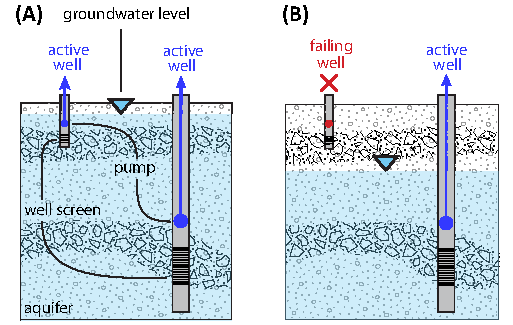
\includegraphics[width=\linewidth]{ch1_figs/fig_conceptual_mod.pdf}
	\caption{Conceptual model of well failure in an unconfined to semi-confined alluvial aquifer (details provided in SI Appendix, \ref{ap_a_formal_wf}). (A) Groundwater level is above all pump intakes, and all wells are active. (B) Groundwater level falls below the pump intake of the shallow well, causing it to fail. The deep well remains active. In our study site, shallow wells tend to be domestic, and deep wells tend to be agricultural and public supply wells.}
	\label{fig:conceptual_model}
\end{figure}


%%%%%%%%%%%%%%%%%%% GW level interpolation
\subsection{Groundwater level interpolation}

Seasonal (spring and fall) groundwater level data for each year between 1998 and 2017 \citep{gwl} were used to determine groundwater level changes in the unconfined to semi-confined shallow aquifer, which domestic wells draw from. For each set of seasonal groundwater levels, we applied ordinary kriging to the log-transformed groundwater levels to normalize the data distribution, suppress outliers, and improve data stationarity \citep{DeutschC.V.andJournel1992, Varouchakis2012}. Because the expected value of back-transformed log-normal kriging estimates is biased (i.e. not equal to the sample mean), we applied the correction of Laurent \citep{Laurent1963, JournelA.G.Huijbregts1978} to recover unbiased groundwater level estimates (SI Appendix \ref{ap_a_gwl}). We further calculated the 5\% and 95\% confidence intervals of the kriging estimates to propagate kriging uncertainty through the model and into the well failure estimates.   


%%%%%%%%%%%%%%%%%%% Pump depth imputation
\subsection{Pump intake depth estimation}

Pump intake depth is not explicitly recorded on WCRs, thus for each well, it was estimated as the mean of the static water level at the time of well completion, and the top of the screened interval (SI Appendix \ref{ap_a_pump_depth}). When pump depth could not be directly calculated (i.e. - a WCRs is missing static water level or the top of the screened interval information), we imputed pump depths with simple linear models to regress known pump depths onto the bottom of the screened interval, which is known for nearly all wells (SI Appendix Figure \ref{fig:pump_loc_bottom}). Pump depth exhibits spatial variance due to geologic heterogeneity and historical groundwater level, hence imputation was conducted at the Bulletin 118 subbasin level (SI Appendix Figure \ref{fig:pump_loc_density}) to ensure hydrogeologic similarity. As with the kriging estimates, we calculated the 5 and 95\% confidence intervals of the estimated pump locations to propagate this uncertainty into the well failure estimates.    

%%%%%%%%%%%%%%%%%%% Calibration
\subsection{Model calibration based on 2012-2016 drought data}

The well failure model was calibrated with observed 2012-2016 well failures by relating groundwater level changes to estimated pump intake locations of wells in OSWCR, and minimizing error between the observed and predicted well failures during the 2012-2016 drought (SI Appendix \ref{ap_a_calib}). Well failures tend to form clusters, thus we calculated Gaussian kernel density estimates for the observed and predicted point patterns and calculated residual error as their difference. We use a kernel bandwidth of 433 $m$, calculated as $0.15 / \sqrt{5 \cdot \lambda}$ where $\lambda$ is the point intensity--the number of observations divided by the study site area \citep{stoyan1994fractals}. Calibration results are depicted at the Public Land Survey System \citep{us2009manual} township resolution (roughly 10 $km$) to improve mapping.




%%%%%%%%%%%%%%%%%%% drought duration scenarios
\subsection{Simulation of drought duration scenarios}

Climate change may cause severe and extended droughts exceeding 4 years in duration, yet the impact of such drought durations on domestic well failure remains unknown. Thus, we simulate drought durations of 5 to 8 years in length by extending the observed 2012-2016 drought with an additional 1 to 4 years using two scenarios:  

\begin{enumerate}
	\item \textit{Continuous drought}: 1 to 4 years of drought immediately following the 2012-2016 drought.
	\item \textit{Intervening wet winter}: identical to the continuous drought scenario, but groundwater levels are allowed to recover after 4 years, due to one intervening wet winter. 
\end{enumerate}

Groundwater level change in each drought duration scenario was determined by assuming that the impact of future droughts is proportional to the historical 2012-2016 drought. In other words, the groundwater level change associated with 1 to 4 additional years of drought is computed by scaling the change in the groundwater level field observed during the 2012-2016 drought by 0.25, 0.50, 0.75, and 1 respectively. 

In the ``continuous drought'' scenario, groundwater levels are already low from the 2012-2016 drought, and increased well failure is expected. Hence, the ``intervening wet winter'' scenario examines how much a wet winter event, such as the one observed in 2017, may buffer against well failure over a longer drought duration.  



%%%%%%%%%%%%%%%%%%% GW management regimes
\subsection{Projected groundwater management regimes}

In California, the Sustainable Groundwater Management Act (SGMA) enacted in 2014, requires the development and implementation of local groundwater management plans by 2020. These plans aim to prevent undesirable results, including the chronic lowering of groundwater levels, to achieve groundwater sustainability by 2040 for critically overdrafted basins.
%, and by 2042 for the remaining high and medium priority basins. 
Overlying landowners of overdrafted basins may deploy different groundwater management regimes, which will impact groundwater level change in the coming decades to various degrees.  

To analyze how different groundwater management regimes might impact groundwater level change and hence domestic well failure, we simulate three simplified regimes for the period 2017 -- 2040 (Figure \ref{fig:SGMAscenarios}): 

\begin{enumerate}
	\item \textit{Strict sustainability}: water levels do not decline after 2020. This represents a theoretical (and idealized) best case management regime for domestic wells.  
	\item \textit{Glide path}: groundwater level decline is gradually reduced over the implementation period until 2040.  
	\item \textit{Business as usual}: groundwater level decline continues at the historic rate. This regime is used for comparison.  
\end{enumerate}


% code/00_figures/alvar_scens
% .R and .ai files: pnas_sgma.ai
\begin{figure}%[tbhp]
	\centering
	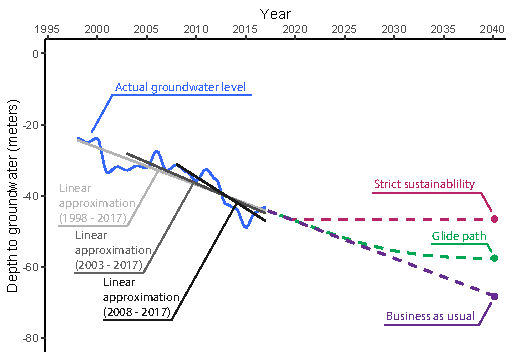
\includegraphics[width=\linewidth]{ch1_figs/fig_sgma.pdf}
	\caption{Projected groundwater management regimes using actual groundwater elevation change for a point in Tulare County as an example. Groundwater level change is approximated by three linear trends, based on different time periods. In this figure, we show the different projected groundwater management regimes using the linear approximation based on the 1998-2017 period. In the analysis, we calculate groundwater levels across the entire CV, using all three trends, and all three regimes.}
	\label{fig:SGMAscenarios}
\end{figure}

To project the number of failing wells for each groundwater management regime, we extend past groundwater level trends through 2040. For this, we first determined past groundwater level trends using data for the period from 1998-2017 and estimated annual groundwater levels at each point of the CV via ordinary kriging as discussed above and in SI Appendix section \ref{ap_a_gwl}. To estimate declining groundwater level trends consistently over time, we only use fall measurements following the growing season. We then obtain linear approximations of groundwater level for each cell using a 5x5 $km^2$ raster. We use three different approximations of groundwater level based on changes observed from 1998-2017, 2003-2017, and 2008-2017 to account for differences in initial groundwater level and thus, uncertainty introduced by the period over which the linear models are built. Finally, to project the ``Strict sustainability'' regime we extend these three approximations into 2020, then eliminate further overdraft. In contrast, the ``Business as usual'' regime projects the linear trends into 2040 before ending overdraft, and the ``Glide path'' regime gradually reduces the slope of the linear trend between 2020 to 2040, representing a middle path between the ``Strict sustainability'' and the ``Business as usual'' regimes. 




%--------------------------------------------------------%
% Results
%--------------------------------------------------------%
\section{Results}

\subsection{Well failure prediction during the 2012-2016 drought}

The calibrated model reproduced both the magnitude and spatial distribution of the 2,027 well failures observed in the study area during the 2012-2016 drought (Figure \ref{fig:pred_obs}A). The model predicts a slightly higher mean number of well failures (n = 2,513) (Figure \ref{fig:pred_obs}B), which is expected, as observed well failures are most probably under-reported due to the voluntary nature of data collection, and a well-owner's perceived consequence of reporting a failed well to their county or state. 

The normally distributed residual error (Figure \ref{fig:pred_obs}C) indicates the unbiasedness and strength of the model: well failure predictions for the observed 2012-2016 drought were within 20\% of the actual value for around 68.2\% of the study area, between 20\% and 55\% of the actual value for around 27.2\% of the study area, and greater than 55\% of the actual value for less than 5\% of the study area. 

Unsurprisingly, both observed and predicted failures tend to cluster in the southeastern CV, where agricultural groundwater use is comparatively higher than elsewhere in the state \citep{Brush2013, Faunted.2009}; households reliant on domestic wells in this region are particularly susceptible to failure. 


% 07_spatial_density_obs_and_pred.Rmd
% code/00_figures/pred_obs/pnas_pred_obs_accuracy.ai
\begin{figure}%[tbhp]
	\centering
	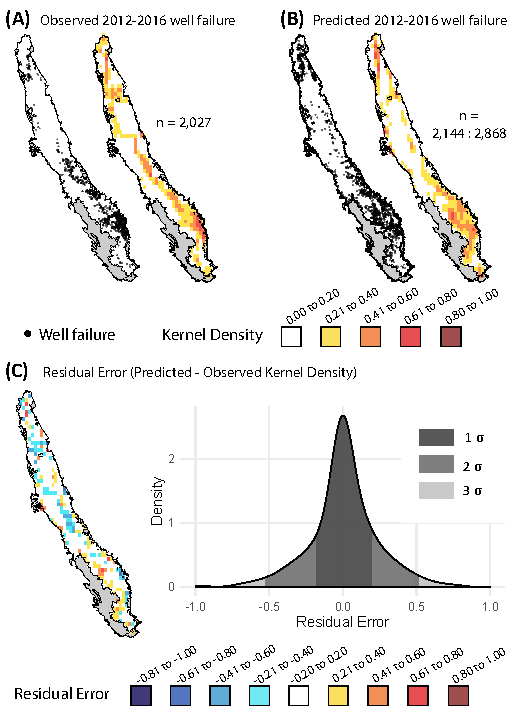
\includegraphics[width=14cm,keepaspectratio]{ch1_figs/fig_pred_obs_accuracy.pdf}
	\caption{Model performance in predicting the spatial intensity of observed domestic well failures during the 2012-2016 drought. (A) Observed well failure point pattern and kernel density estimate. (B) Predicted well failure mean estimate (n = 2,513) and kernel density of the mean prediction. The 5 and 95\% confidence intervals of predicted well failures span the interval from 2,144 - 2,868. (C) Residual (predicted minus observed) error, with red areas indicating areas of over-prediction, and blue areas indicating under-prediction.}
	\label{fig:pred_obs}
\end{figure}



%%%%%%%%%%%%%%%%%%% Drought duration scenarios
\subsection{Failing and vulnerable wells in drought duration scenarios}

Longer drought duration results in widespread well failure episodes concentrated primarily in the southeastern CV (Figure \ref{fig:p_1_2_3_4}). Consistent with domestic well failure patterns observed during the 2012-2016 drought, well failure density is highest in Madera, Kings, Kaweah, Tule, Tulare Lake, and Kern subbasins.  

% pred_1_2_3_4 in `09_plot_pred_future_failures.Rmd`
% density_pred_1_2_3_4 in `09_plot_pred_future_failures.Rmd`
% code/00_figures\pred_1_2_3_4/pnas_pred_1234_small_2.ai
\begin{figure}%[tbhp]
	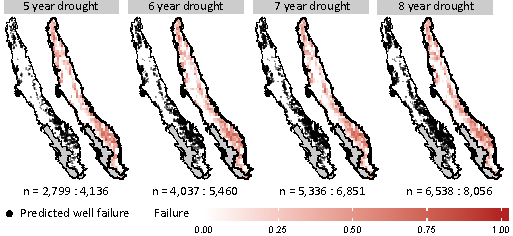
\includegraphics[width=\linewidth]{ch1_figs/fig_pred_1234_small_2.pdf}
	\caption{Simulated domestic well failure point patterns and associated kernel density estimates for 5 to 8 year drought duration scenarios beginning in Fall 2016 (maps show mean prediction). $n$ is the 5 and 95\% confidence interval of cumulative well failure count in each scenario, including the 2,027 failing wells in the 2012-2016 drought.}
	\label{fig:p_1_2_3_4}
\end{figure}

In the ``continuous drought'' simulation, two- and four-year long droughts immediately following the 2012-2016 drought (6 and 8 years total without an intervening wet winter) result in 4,037 to 5,460 and 6,538 to 8,056 cumulative well failures, respectively. Thus, a two-year drought duration following the 2012-2016 drought results in more well failures than the 2012-2016 drought alone, and a combined 8 year drought duration results in nearly twice the failures observed from 2012-2016 (Figure \ref{fig:cum_sum_failure}). Intensified well failure during extended drought reinforces the interdependence of well failure on groundwater level: when groundwater levels cannot recover to pre-drought levels and pump depths are fixed, wells are more vulnerable to failure.  

% `cum_sum_failures.pdf` in figures/code
% `p` in `13_trendline_d-2012_2016_and_future_d.Rmd`
% code/00_figures/cum_sum_fail/pnas_cum_sum_fail.ai
\begin{figure}%[tbhp]
	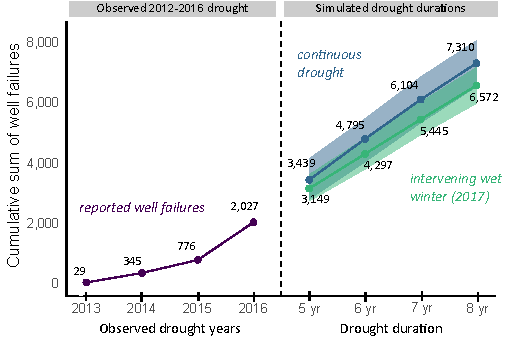
\includegraphics[width=\linewidth]{ch1_figs/fig_cum_sum_fail.pdf}
	\caption{Left: Cumulative domestic well failures from 2012-2016. Right: Cumulative domestic well failures resulting from simulated drought durations 5 to 8 years in length. The continuous drought duration scenario (blue) leads to more well failure compared to the intervening wet winter scenario (green). Points represent the mean well failure estimate, and shaded regions represent the 5 and 95\% confidence intervals. %Observed well failures from 2012-2016 reflect when the failure was reported, not necessarily when the well actually failed. Data collection by the state did not begin in a systematic way until late 2014, and many of the reports received in 2016 may be motivated by the fact that the state made financial assistance available to households on private wells in this year.
	}
	\label{fig:cum_sum_failure}
\end{figure}


In the ``intervening wet winter'' scenario, groundwater levels are allowed to recover during 2017, and well failure slightly abates: 498 and 738 fewer wells fail in the 6 and 8 year drought scenarios, indicating that an increase in median groundwater level of only a few meters across the Central Valley can prevent hundreds of domestic well failures during extended drought.  

%The cumulative sum of annual well failures observed during the 2012-2016 drought follows an exponential trend; in simulated extended drought scenarios, it follows a linear trend (Figure \ref{fig:cum_sum_failure}). If the drought were to continue past the simulated 8 years scenario, well failures would follow a sigmoidal trend: inflecting then leveling off, as failure progresses to increasingly infrequent and deeper wells until none are left.  

The cumulative sum of annual well failures observed in the evaluated drought duration scenarios follows a linear trend (Figure \ref{fig:cum_sum_failure}). If the drought were to continue past the simulated 8 years scenario, well failures likely would follow a sigmoidal trend: inflecting then leveling off, as failure progresses to increasingly infrequent and deeper wells until none are left.  

Vulnerable wells (Figure \ref{fig:vi}) are those with estimated pump intakes within 3 $m$ of the groundwater level, and are at heightened risk of experiencing a reduction in pump efficiency, or a failure episode. Since this 3 $m$ window is fixed in our analysis, the spatial distribution and count of vulnerable wells is relatively constant across the drought duration scenarios (2,274 to 2,453 wells), and the present day scenario of Fall 2018 (mean estimate = 2,568). Moreover, the spatial distribution of vulnerable wells mirrors those of well failures.

% figure starts in code/15_vulnerability_index.R
% 00_figures/vi/pnas_vi.ai 
\begin{figure}
	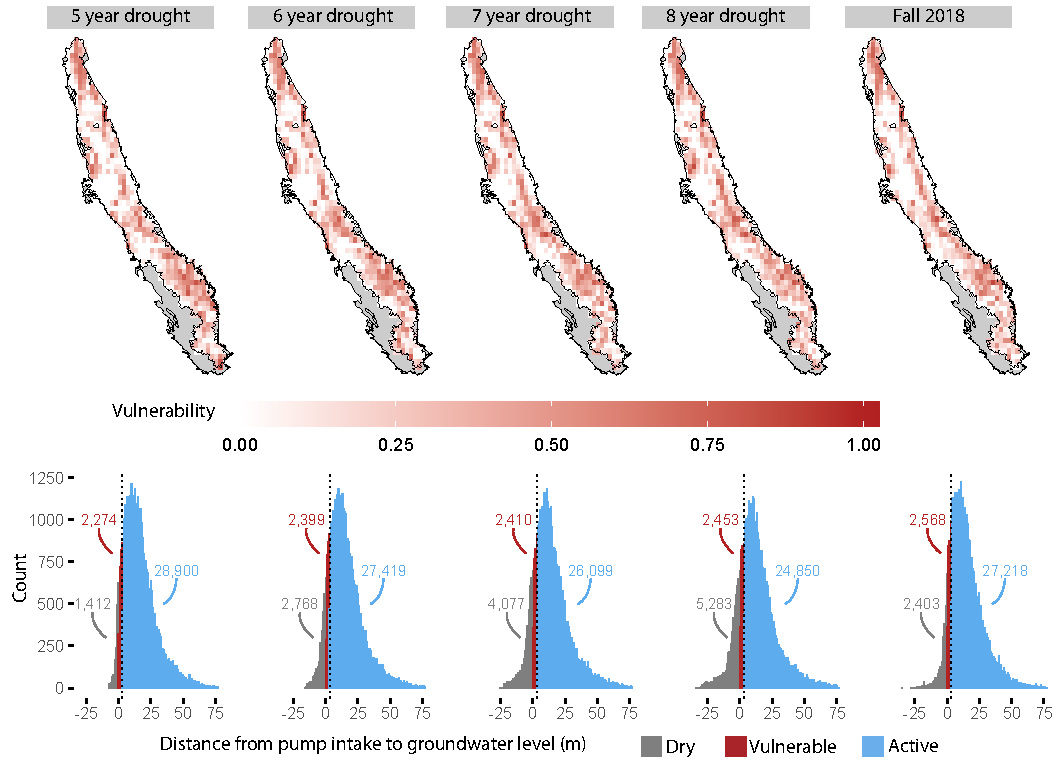
\includegraphics[width=17.8 cm]{ch1_figs/fig_vi.pdf}
	\caption{Top row: kernel density estimates of low vulnerability (white) and high vulnerability (red) regions in extended drought duration scenarios and in Fall 2018. Bottom row: histograms of failing wells (grey), vulnerable wells (red), and active wells (blue) for the extended drought scenarios and Fall 2018 scenario. The black dotted line at 3 meters is the threshold at which wells are at risk of decreased efficiency. All numbers reported are the mean estimate of dry, vulnerable, and failing wells.}
	\label{fig:vi}
\end{figure}



%%%%%%%%%%%%%%%%%%% sustainable management regimes
\subsection{Failing wells in projected groundwater management regimes}

Projecting groundwater depths into 2040 under three different management regimes results in significant differences in domestic well failures (Figure \ref{fig:sgma_grid}). The ``Business as usual'' regime, with no change in the historical trend of groundwater level decline, would lower the groundwater level by up to 100 $m$ in parts of the southern CV, but significant groundwater level declines are widespread. Scenarios aimed at achieving sustainability would reduce these declines, hence the differences between the ambitious ``Strict sustainability'', ``Glide path'' and ``Business as usual'' pathways might be quite important for water resources managers and policy makers.

The groundwater depth changes and associated well failures are sensitive to the period used for the linear approximation of groundwater level declines. The period from 2008-2017 leads to significantly worse groundwater depletion than both periods 2003-2017 and 1998-2017, particularly because of the effects of the 2012-2016 drought. Average well failures for the ``Business as usual'' regime range from 5,966 to 10,466 (depending on the period used for the linear interpolation), while under the ``Glide Path'' regime they range from 3,677 to 6,943, and from 1,516 to 2,513 under the ``Strict sustainability'' regime (confidence intervals are reported in SI Appendix Table \ref{tab:dom_failures}).  

% 18_run_model_2.R for simulation and plotting. paths below outdated.
% 00_figures/alvar_scens/pnas_sgma_grid_trim.ai
% 12_sustainable_gw_mgnt_scenarios.Rmd for:
% pnas_sgma_gwl_change.pdf | pnas_sgma_gwl_change_grid.pdf
% pnas_sgma_dry_wells.pdf | pnas_dry_well_grid.pdf
% 00_figures/alvar_sgma/sgma_scens.R for pnas_sgma_trends.pdf
\begin{figure}
	\includegraphics[width=17.8 cm]{ch1_figs/fig_sgma_grid_trim.pdf}
	\caption{Domestic well failures projected for three groundwater management regimes (columns) based on three different time periods of linear groundwater level change (rows). The left plot of each pair is the mean projected groundwater level change from 2017-2040. Groundwater level decline (red) is more common than groundwater level increase (blue). The right plot of each pair shows the mean predicted well failure point pattern for that combination of groundwater management regime and groundwater level change approximation. See SI Appendix Table \ref{tab:dom_failures} for confidence intervals.}
	\label{fig:sgma_grid}
\end{figure}
%TC:endignore
\clearpage

Most of the estimated domestic well failures are still concentrated in the southeastern CV, but the central and northern CV are also affected, presumably due to the ubiquity of relatively shallow wells in these regions. The ``Business as usual'' regime leads to especially severe well failure in all three projected groundwater level trends.



%--------------------------------------------------------%
% Discussion
%--------------------------------------------------------%
\section{Discussion}


%%%%%%%%%%%%%%%%%%% 
\subsection{Impact of drought duration on well failure and vulnerability}

It is well understood that drought duration leads to increased groundwater extraction \citep{Hanak2011, Medellin-azuara2016}, and hence domestic well failure \citep{Perrone2017, Feinstein2017}. Thus, we tested the impact of previously unseen drought durations ranging 5 to 8 years in length, by simulating an additional 2 to 4 years of severe drought immediately following the 2012-2016 drought, calculating the change in groundwater level, and determining failing and vulnerable wells. 

%Unlike existing regional-scale analyses \citep{Perrone2017}, the domestic well failure model developed in this study improves upon existing well failure models in terms of spatial scale \citep{Gailey2019}, and allows for scenario testing. 
A previous study estimated that 4 years of drought in the Tulare County, California immediately following the 2017 wet winter would result in about 200 - 850 domestic well failures \citep{Gailey2019}. 
Our model's equivalent scenario (intervening wet winter with an 8 year drought duration) results in a similar range of 585 - 715 domestic well failures in Tulare County. Additional comparisons are not possible given the lack of research on this topic.  

At the level of California's CV, our results suggest that drought durations of 6 to 8 years result in 4,037 to 5,460 and 6,538 to 8,056 cumulative well failures, respectively. However, an intervening wet winter during the 6- and 8-year long drought duration simulations buffers against well failure: when groundwater is allowed to recover after 4 years of drought (as happened during the 2017 wet winter), an average of 498 and 738 less domestic wells fail. These findings support research indicating that limiting groundwater pumping during drought may reduce well failure \citep{Hanak2019, Gailey2019}, and a general understanding that groundwater pumping can lower proximal groundwater levels \citep{theis1935relation}.  

During the 2012-2016 drought, the median groundwater level in the CV fell to progressively new historic lows each fall after the summer growing season (SI Appendix \ref{ap_a_drought_impact}) \citep{dwrgwl2017}. Our results indicate that between fall of 2014 and 2015, the median groundwater level across the entire CV fell by nearly 5 $m$, and in some areas (i.e. - Tulare, Kings, and Kern counties), by tens of meters. In fall of 2016, the median groundwater level in the CV was 27.0 $m$ below land surface. Moreover, our results indicate that the interquartile range of domestic well pump locations in the CV is 24.5 to 52.3 $m$ below land surface. The proximity of pump intake depths to groundwater levels explains why domestic wells are sensitive to even slight declines in groundwater level: 5 to 10 $m$ of groundwater level decline may easily impact thousands of domestic well pump intakes and cause failure. 

In the four drought duration scenarios evaluated, an average of 2,274 to 2,453 domestic well pumps reside within 3 $m$ of the groundwater level. We classified these wells as vulnerable, because they are likely to fail first under persistent groundwater level decline. The spatial distribution of well vulnerability mirrors that of well failures. Mapping clusters of predicted failing and vulnerable wells is essential for sustainable water management and disaster response.


%%%%%%%%%%%%%%%%%%% 
\subsection{Implications for groundwater management and policy}

The strong dependence of domestic well failure on groundwater pumping to support irrigated agriculture raises serious questions concerning the role of sustainable groundwater policy in mitigating well failure \citep{Hanak2019}. We evaluated three different projected groundwater management regimes to curb groundwater level declines in the coming years: a ``Strict sustainability'' theoretical best-case regime wherein declining trends in groundwater level stop in 2020, a ``Business as usual'' regime that continues groundwater decline until 2040, and a final ``Glide path'' moderate regime that slows the rate of groundwater level decline to the midway point between the former two regimes.  

Our results suggest that choices embedded within each of the groundwater management regimes vastly impact the amount of expected well failures. For instance, the ``Glide path'' regime predicts 3,677 to 6,943 domestic well failures by 2040, and the ``Business as usual'' regime predicts 5,966 to 10,466 domestic well failures by 2040. Both groundwater management regimes would result in twice to almost three times as many well failures than the ``Strict Sustainability'' regime (1,516 to 2,513 failures). All three scenarios are sensitive to the period of record used to approximate the linear groundwater level decline, however they underpin the vulnerability of domestic wells to historic rates of groundwater level decline, and demonstrate the impact of management on well failure.  

Refilling overdrafted aquifers via managed aquifer recharge might meet the dual objectives of increasing groundwater storage, and bolstering domestic well dependent households' drought resilience. In California, high-magnitude flood flows are likely the most accessible and largest sources of water to replenish groundwater aquifers through managed aquifer recharge \citep{Kocis2017}, which might considerably slow or reverse trends in groundwater depletion. The emerging research in the strategic siting of managed aquifer recharge considers impacts on crop health \citep{Dahlke2018}, human health \citep{ayuso2011quantifying}, the mobilization of contaminants into groundwater \citep{Xanke2017}, and hydrogeologic suitability (i.e. - highly conductive flowpaths and geologic formations capable of accommodating large volumes of water, such as incised valley fills) \citep{Maples2019}. In the San Joaquin Valley where domestic well failures peak, managed aquifer recharge alone may not be enough to offset groundwater overdraft, but coupled with a reduction in agricultural water use \citep{Hanak2019}, groundwater levels may stabilize enough to prevent widespread future failure events. 

This study assumes that no interim well construction takes place to prepare for falling groundwater levels, such as the practice of pump lowering or well deepening. Pump lowering typically takes place in 6 $m$ intervals (the length of standard discharge piping), and costs around \$2,000 USD per lowering event \citep{Gailey2019}. If we consider the cost of pump lowering in all failing wells in the 6- and 8-year drought duration scenarios (in reality some wells will not have room to be lowered) and assuming every failing well's pump is lowered once (some will require more than one lowering), at \$2,000 USD per 6 $m$ unit of discharge piping, 4,037 - 5,460 and 6,538- 8,056 failures correspond to \$8.7 - \$10.4 and \$13.8 - \$15.5 million USD. 

During the recent drought, it is likely that some households also deepened their wells. In California and nationwide, drilling deeper wells is a common practice to adapt to declining groundwater levels \citep{Perrone2019}, but is a costly and unsustainable solution that may furthermore result in cross-contamination due to interconnection of confined aquifers by well construction \citep{gailey2017inactive}. Moreover, the financial burden of pump lowering or well deepening might disproportionately impact disadvantaged populations \citep{Famiglietti2014} unable to afford chasing after declining groundwater levels. Since many of these disadvantaged groups may not own their land and thus wells, well construction decisions may be made by landowners rather than the affected groups.  

%%Underpinning the dilemma of domestic well failure is the urgent need for an adequate cost estimation to facilitate sensible short- and long-term policy solutions. 
Sustainable long-term solutions for drinking water access might include connecting vulnerable households to nearby centralized water provisions. Recent research indicates that many rural communities, assumed to be on domestic wells, are actually quite close (less than 2 $km$) to a potable water supply system \citep{London2018}. However, as annexation and consolidation is financially and physically impractical for all domestic-well dependent households, many will remain too remote and isolated to connect to a nearby water system.  

%We currently lack a thorough understanding of the economic burden of well failure and how it may affect demographic groups disproportionately. 
Short- and long-term solutions to domestic well failure remain largely unexplored. What role can managed aquifer recharge play in mitigating well failure? Given the strong dependence of groundwater level decline on extraction for irrigated agriculture, could agri-business proximal to centers of high well failure collectively fund safety nets that internalize the cost of well failure during periods of increased groundwater pumping? Should vulnerable domestic well reliant populations connect to nearby municipal water systems with more reliable water supply? What is the appropriate solution for those that are too remote or isolated to connect to a community system? 

%%%%%%%%%%%%%%%%%%% 
\subsection{Applicability to other areas}

The well failure model presented in this study is extensible to other areas outside of California where sufficient data or groundwater flow models are available. It relies on two inputs: (1) a time series of spatially-explicit groundwater level surfaces reflecting typical groundwater level changes (specifically, the maximum drawdown), and (2) well construction information (i.e. - geographic location and pump intake depth). 

Approaches for interpolating groundwater levels and estimating pump intake depths are demonstrated in this study, though others exist \citep{Gailey2019, Perrone2017, OSullivan2010, JournelA.G.Huijbregts1978}. Groundwater levels provided by a groundwater flow model such as MODFLOW \citep{Harbaugh2000} would easily couple to a well failure model, enabling the simulation of water management regimes and the impact of the resulting groundwater level on domestic well failure at arbitrary temporal scales. In California, existing regional-scale groundwater flow models such as C2VSim \citep{Brush2013} and CVHM \citep{Faunted.2009} can be used to plan for the impact of future failure episodes under different water management regimes involving changes in both pumping and recharge in space and time. 

This study aimed for regional prediction of failing, vulnerable, and active wells, but more nuanced impact analyses can be made. For instance, variable losses in well efficiency may be quantified as groundwater levels fall \citep{Medellin-azuara2016}. This in turn enables the cost estimation of repairing failing and vulnerable wells (e.g. - pump lowering, well deepening), compared to water management actions (e.g. - fallowing fields, reduced groundwater pumping).  

Where resources exist to survey households, detailed domestic well information such as geographic location, pump intake depth, and retirement age may be obtained, and would further constrain the uncertainty inherent in the estimation of these parameters. Additionally, well failure observations are essential for model calibration. Though this study benefited from failure data, efforts to anticipate domestic well failures as proactive hazard mitigation should not wait for the existence of observational data. It does, however, suggest the benefit of having such a system in place as part of local and state-level drought preparedness.  

%%%%%%%%%%%%%%%%%%% 
\subsection{Implications for adaptation to climate change}

Our results demonstrate that the mechanisms leading to domestic well failure are heavily dependent on groundwater level declines due to pumping for irrigated agriculture and increased pumping during drought. A historical lack of groundwater management in California \citep{Hanak2011} has led to widespread groundwater level decline. Climate change compounds the impact of water management decision-making. Warming will increase the frequency and duration of drought in California and other parts of the world \citep{Diffenbaugh2015, Cook2015, Swain2018, Rhoades2018, VanLoon2016}, and if left unchecked, groundwater withdrawal will likely intensify as surface water becomes more scarce, as it has in the past \citep{Hanak2011}. As we demonstrate in this study, groundwater replacement of lost surface water during extended drought intensifies well failure due to already low groundwater levels. Thus, managing for low to no domestic well failure requires a consideration of the complex interaction between land use change, water resources management, human decision-making, and climate change. Unless adaptation strategies become integral to sustainable groundwater management policy, the extended droughts anticipated under climate change and resulting changes in groundwater levels will put thousands of domestic wells in California's CV at risk of failure, and hence, thousands of Californians at risk of losing access to water.  


%%%%%%%%%%%%%%%%%%% 
\subsection{Additional perspective on the data and model}

%% This study is one example of how state-led initiatives towards open data, or the practice of releasing previously-private databases to the public, enables research towards previously inaccessible questions. This study benefited from open data tabulated in a machine-readable format, which simply would not have been possible otherwise. By comparison, while former studies have dedicated many hours to statistically sample and manually read nearly three quarters of a million WCRs \citep{Johnson2015}, we were able to automate the reading and QAQC process for nearly one million tabulated WCRs. This reinforces existing and nascent efforts to transition data-collection and storage to standardized, digital, and machine-readable formats that can be easily accessed and manipulated by scientific scripting languages.  

There is generally good agreement between the observed and predicted well failure at the 10 $km$ resolution of the residual error maps (Figure \ref{fig:pred_obs}A-B), and better agreement (Figure \ref{fig:pred_obs}C) is achieved at larger spatial scales (i.e. - Bulletin 118 groundwater subbasins, entire CV). Thus, the results presented in this study should not be taken as \textit{de facto} predictions of the exact locations of well failure, but rather, as \textit{regional-scale} well failure estimates. Local-scale errors introduced by uncertainty in well failure reporting, well completion reporting, groundwater level, and model formulation are overcome at regional scales. 

We acknowledge that spatial and temporal variability in monitoring well data introduces uncertainty in the interpolated groundwater level. Ambient monitoring wells measured each season (i.e. - spring and fall) are not the same across seasons, and each season's measurements are sampled over a roughly three month time frame (January-March in the spring, and October-December in the fall). However, because most of the groundwater level change observed in a year takes place as the result of the summer growing season, and the fall measurements take place after the summer, spring and fall measurements still reflect ambient conditions. Moreover, both scaling the 2012-2016 groundwater level change to create future drought scenarios, and calculating 2040 groundwater levels with linear trends are simple approaches to estimate future groundwater level decline, but the accuracy of any method to forecast unseen future events are also questionable. Additionally, we do not account for any emergency response measures in response to drought such as groundwater pumping curtailments. In California, some households were able to drill deeper wells, lower their pumps, or connect to a nearby surface water supply system during the drought. Because these corrective actions are cost-prohibitive and highly unlikely to be widespread, our modeling assumptions (no corrective action) and hence results, still agree with observed well failure rates from 2012-2016. 




%--------------------------------------------------------%
% Conclusion
%--------------------------------------------------------%
\section{Conclusions}

%% More than one million Californians rely on private domestic wells for drinking water, and nearly half a million of these people live in the CV. Owing to their relatively shallow depth, domestic wells often fail first when groundwater levels fall, as observed during the 2012-2016 drought. As water resource managers aim to stabilize groundwater level declines, climate warming threatens to increase drought frequency and duration in California. We currently lack drought preparedness tools for regional-scale estimation of domestic well failure, and the ability to rapidly assess future well failure under different groundwater level scenarios. 

In this study, we developed a data-driven well failure model and applied it to California's CV to make regional-scale estimates of domestic well failure, and assess future well failure under different groundwater level scenarios.  

Our model reproduces reported domestic well failures during the 2012-2016 drought in California's CV ($n$ = 2,027), and furthermore, simulates the impact of different drought duration scenarios up to 8 years in length. We show that small declines in groundwater level are sufficient to cause thousands of wells failures when groundwater levels are already low, and that wet winters, and hence groundwater recharge or reduced pumping, may buffer against well failure. A simulated drought duration of 6 years (2012-2018) results in 4,037 - 5,460 total well failures. Similarly, an 8-year long drought (2012-2020), corresponds to a median groundwater level change of less than 10 $m$ across the CV, but results in 6,538- 8,056 total well failures. The same 6 and 8 year long drought duration scenarios with an intervening wet winter in 2017 lead to an average of 498 and 738 fewer well failures. Lastly, wells that do not fail may still be vulnerable to failure. Our model estimates that in Fall 2018, an average of 2,568 well pump intakes were within 3 $m$ of the groundwater level, and 10,544 well pump intakes were within 10 $m$ of the groundwater level. 

Our model further shows that early adoption of sustainable groundwater management regimes aimed at halting declining trends in groundwater level will lessen the magnitude of domestic well failure. A ``Business as usual'' linear groundwater level decline would result in an average of 5,966 - 10,466 domestic well failures by 2040. In contrast, a more gradual ``Glide path'' decline would result in 3,677 - 6,943 domestic well failures by the same date. A ``Strict sustainability'' regime that allows groundwater levels to decline until 2020 before halting would result in 1,516 - 2,513 well failures.  

Together, these results demonstrate that access to domestic water supply for large rural populations may be imperiled by a relatively small number of agricultural users, posing challenges for equitable and sustainable groundwater management which may not adequately represent domestic well users. 

Models like the one developed in this study may be updated over time to accommodate additional wells, refine existing well construction information, and evaluate the impact of potential water management strategies on groundwater level changes, and hence well failure. This study's approach to well failure modeling may be applied in other arid regions worldwide to facilitate drought preparedness planning. We anticipate that the model developed herein may be used by local and state agencies developing groundwater management plans in accordance with California's Sustainable Groundwater Management Act.  

\clearpage
 %This looks for chapter2.tex
%%%%%%%%%%%%%%%%%%%%%%%%%%%%%%%%%%%%%%%%%%%%%%%%%%%%%%%%%%%%%%%%%%%%%%%%%%%%%
\section{Supporting Information Appendix} \label{ap_a_dom_wells}

\subsection{Study Area}
\label{ap_a_study_area}

The study area was pared down from the Central Valley (CV) to only the area where more recently completed domestic wells (1976 and younger) were present. This cutoff was chosen because the model period in this study ends in 2016, thus wells completed on or after 1976 ($n = 67,011$) assumes a conservatively high well retirement age of 40 years. Circular, 5 $km$ buffers were drawn around each well, then joined to create a unified study area polygon. Some isolated circles that were not connected to any other buffers ($<$ 1\% of the buffered area) were removed in order to constrain the study site to one contiguous spatial extent in the CV corresponding to the areas of greatest domestic well density. The small removed areas principally occur in the western San Joaquin Valley. Low rates of domestic well completion in the west side of the San Joaquin Valley compared to the CV as a whole are explained by a relatively deep water table, poor shallow groundwater quality, and perhaps missing well completion records in places where there are actually households on unregistered or non-permitted domestic wells. 


%%%%%%%%%%%%%%%%%%%%%%%%%%%%%%%%
\subsection{Data}
\label{ap_a_data}

The California DWR keeps paper records of wells drilled in California that contain well construction information, such as the depth of the well, perforated interval dimensions, location, and well type (e.g. - irrigation, domestic, monitoring, etc.) among other data. These records are submitted by the well-drilling company to the state in the form of a Well Completion Report (WCR). Nearly all WCRs in the state have been digitally scanned, and key fields in the reports have been digitized. Until recently, WCR information was confidential under state law, and they were unavailable to the general public, limiting researchers' abilities to answer questions like those set forth in this study.

The State’s Household Water Supply Shortage Reporting System (HWSSRS) was established in late 2014 as a tool to capture information on water supplies running dry due to worsening drought conditions across California. The data gathered by the system was used for coordinating the State’s drought emergency response efforts.  The system was set up as a voluntary, self-reporting system and, as such, only represents some fraction of the actual water supply shortages occurring. Most of the reported shortages were dry wells, but some were streams. Most of the reports were actually received by county health officials who entered the data into the system. Some counties were very active in reporting, while some were not. A download of the reported HWSSRS data has been made available to researchers with redaction of some data fields and a reduction in the accuracy of geospatial data to protect personal identification. The precision of the geospatial data is 36 arc seconds, corresponding to approximately 1 $km$ in the study area. The coordinate reference system used in this study is EPSG 4326.  

The great majority of well locations in OSCWR ($>$ 95\%) are rounded to the nearest centroid of the Public Land Survey System (PLSS) section. The PLSS is composed of a nested series of cadastral surveyed lands (e.g. townships, range and sections). Townships measure 6x6 square miles (93.24 $km^2$ each) in size and are made up of thirty-six one-square mile sections (2.56 $km^2$). As the distance between the cell centroid and a corner of each section is the half-diagonal $0.5\cdot\sqrt{2}\cdot1.6 = 1.14$ $km$, the reported location \textit{(x, y)} of each well is always 0 $\leq$ \textit{(x, y)}  $\leq 1.14$ $km$ from the true location. Determining the exact location of a well from the scanned well completion reports is intractable as well coordinates are rarely provided on the scanned forms, and the listed street address typically corresponds to the well owner's residence, not necessarily where the well is located, thus hampering efforts at geocoding. Due to these limitations, the reported PLSS section centroid was taken as the approximate well location, with a maximum error of 1.14 $km$.

%%%%%%%%%%%%%%%%%%%%%%%%%%%%%%%%
\subsection{Formal evaluation of well failure}
\label{ap_a_formal_wf}

Classification into active wells and failing wells proceeds through several steps (Figure \ref{fig:tree}). Consider a well $i$. It has a set of spatial coordinates and an associated estimated pump depth $(x_i,y_i,z_i)$, where $x_i$ and $y_i$ are the Cartesian coordinates, and $z_i$ is the estimated depth of the pump within the well casing that draws water from the surrounding aquifer. The groundwater level $g$ is a scalar field which varies by location; the groundwater level at a well is thus a scalar defined by its coordinates: $g_i = f(x_i,y_i)$. We determine the groundwater level for some initial time $g({t_0})$ and final time $g({t_f})$ at each location in the study area by ordinary kriging.  

% tree diagram of well failure
\begin{figure}[ht]%[tbhp]
	\includegraphics[width=17.8 cm]{ch2_appendix_figs/tree.png}
	\caption{Decision tree representing the steps taken to evaluate active and retired wells, initially active and well failures, and finally, active wells and well failures given the following boundary conditions: retirement age, initial groundwater level, and final groundwater level.}
	\label{fig:tree}
\end{figure}

Classification into active and failing wells proceeds as follows. Let the set of all domestic WCRs be called $W$. First, wells with age $a$ greater than or equal to the calibrated retirement age $t_r$ (Section \ref{ap_a_calib})
 are removed from the simulation. 
%(see section \ref{ss_2_6} for a discussion of how this parameter is determined). 
This yields two sets: the initial wells to consider ($W_i$), and the retired wells ($W_r$).  

$$W_i \subseteq W : a_i \leq t_r$$  

$$W_r \subseteq W : a_i > t_r$$  

The remaining active wells at this point are the initial wells to consider, $W_i$. However a well may not be active at $t_0$ frame if its pump is above the groundwater level at $t_0$. Next, wells with pumps above the groundwater level at the start of the simulation were removed, yielding another two sets: the active wells at time zero $W_a(t_0)$, and the failing wells at time zero $W_d(t_0)$. 

The active wells at time zero are the subset of initial wells to consider where the groundwater level at time zero $g({t_0})$ at the location of the well exceeds the pump depth $z$, and the failing wells at time zero are the wells where the groundwater level at time zero at the location of the well falls at or below the pump depth.  

$$W_a(t_0) \subseteq W_i : g({t_0}) > z$$  

$$W_d(t_0) \subseteq W_i : g({t_0}) \leq z$$

Lastly, the groundwater level field at the final time $g({t_f})$ is applied, yielding the final two sets of wells: well failures $W_d(t_f)$ and active wells $W_a(t_f)$. Well failures are the subset of wells where the final groundwater level at the location of the well falls at or below the level of the pump, and active wells are the subset of wells where the final groundwater level at the location of the well does not fall below the level of the pump.  

$$W_a(t_f) \subseteq W_0 : g({t_f}) > z$$  

$$W_d(t_f) \subseteq W_0 : g({t_f}) \leq z$$  

$W_d(t_f)$ and $W_a(t_f)$ combined form the set of all active wells at time zero $W_a(t_0)$. 

Taken together, the three steps taken to classify wells into active and failing wells are visualized as a decision tree in Figure \ref{fig:tree}.  


%%%%%%%%%%%%%%%%%%%%%%%%%%%%%%%%
\subsection{Vulnerable wells}
\label{ap_a_vi}

Vulnerable wells are defined as wells that may experience a loss in function due to sufficiently low water levels above the estimated pump intake depth. We estimate that 3 $m$ is the threshold at which a well may experience losses in function, based on a pumping rate of 1 $m^3 / hr$, a required net positive suction head of 5 $m$, a barometric pressure head of 10 $m$ (at 25 degrees C and 0 $m$ above mean sea level), a vapor pressure (at 25 degrees C) of 0.3 $m$, and friction head losses of 1 $m$ \cite{Tullis1989}. 


%%%%%%%%%%%%%%%%%%%%%%%%%%%%%%%%
\subsection{Groundwater level interpolation}
\label{ap_a_gwl}

The groundwater level interpolation consists of five steps: (i) data collection; (ii) log transformation; (iii) ordinary kriging; and (iv) back-transformation and correction of the interpolated groundwater levels.  
Groundwater level data covering fall and spring measurements between 1998 and 2017 were obtained from DWR \cite{gwl}. Seasons are defined as either spring (January - March) or fall (August - October). Groundwater levels in a season reflect the ambient signal of the unconfined to semi-confined aquifer. Groundwater levels are measured in reference to the land surface at the measurement locations.

Many environmental data follow a log-normal distribution \cite{Stedinger1980}, including the ambient groundwater levels used in this study. Depths to groundwater at each monitoring well were log transformed ($ln(x)$) prior to interpolation to normalize the data distribution, suppress outliers, and improve data stationarity \cite{DeutschC.V.andJournel1992, Varouchakis2012}. 

Ordinary kriging was then used to interpolate groundwater levels for each season. Inverse distance weighting and thin plate splines were also considered, but discarded because they produced unrealistic groundwater levels near the study area's boundaries, where conditioning data was sparse, and unlike kriging, are susceptible to bulls-eye patterns (concentric areas of equal value around known data points).  
%The interpolation techniques used in this study are well documented (e.g. \cite{JournelA.G.Huijbregts1978}) and beyond the scope of this paper. 
Ordinary kriging parameters were determined by fitting an exponential semi-variogram model. 

Since the expected value of back-transformed log-normal kriging estimates is biased (i.e. - not equal to the sample mean), we apply a correction \cite{Laurent1963, JournelA.G.Huijbregts1978}:  

\begin{equation}
    g = k_0 \cdot exp \Big[ ln(\hat{g}_{OK}) + \frac{\sigma^2_{OK}}{2} \Big]
\end{equation}

Where $g$ is the corrected and back-transformed groundwater level, $\hat{g}_{OK}$ is the ordinary kriging estimate, $\sigma^2_{OK}$ is the kriging variance, and $k_0$ is the correction factor, proportional to the ratio of the mean of the sample values to the mean of the back-transformed kriging estimates.  

Lastly, the the 5 and 95\% confidence intervals of the kriging estimate was determined via: $\hat{g}_{OK} \pm (1.96 \cdot \sqrt{(\sigma^2_{OK})})$. These confidence intervals are propagated through the model to account for uncertainty in the estimated groundwater level.   


%%%%%%%%%%%%%%%%%%% GW levels
\subsection{Impact of drought on seasonal groundwater levels}
\label{ap_a_drought_impact}

Interpolated seasonal groundwater levels in the study area during the 2012-2016 drought exhibit oscillating seasonal variation between spring and fall, a downward trend as the drought progresses from spring 2012 to fall 2015, and an upward trend beginning in spring 2016 and continuing into 2017. Seasonal groundwater level oscillation is a byproduct of agricultural groundwater demand, which peaks during summer and fall months. 

% gw_boxplot_sp_fall in `02_interpolate_all_seasons_GF.Rmd`
% sp_fa_gwl in `06_calibartion_herve_alvar_graham.Rmd`
% sp_fa_gwl.ai in code/00_figures/sp_fa_gwl/pnas_sp_fall_gwl.ai
\begin{figure}[ht]%[tbhp]
	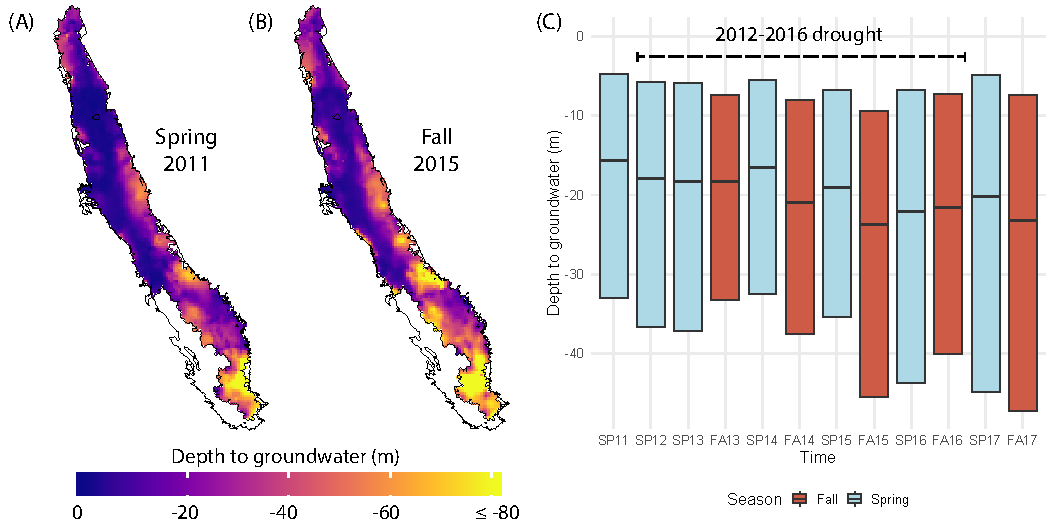
\includegraphics[width=17.8 cm]{ch2_appendix_figs/erl_sp_fa_gwl.pdf}
	\caption{Groundwater levels during the most intense 4-year period of the 2012-2016 drought in (A) spring 2011, and (B) fall 2015. (C) Box plots showing the median and 25\% and 75\% percentiles of depth to groundwater. Compared to spring groundwater levels, fall levels tend to be deeper. The schematic assumes that groundwater levels do not decrease with depth, which is not a concern for most of the domestic wells because they tend not to be very deep.}
	\label{fig:sp_fall_gwl_2}
\end{figure}

The median groundwater level oscillates with the growing season (Figure \ref{fig:sp_fall_gwl_2}C) and is generally higher in spring than in fall of the same year. Between spring and fall of 2015 alone, the median groundwater level across the CV fell by nearly 5 $m$. In that same water year, Sierra snowpack measured at an all time low of 5\% of the average snowpack \cite{cadwr2017}, implying that low snowpack leads to more groundwater pumping and hence a seasonal lowering of groundwater levels. 

Median groundwater levels decline between spring 2012 and fall 2015, the four driest consecutive years on California's record (Figure \ref{fig:sp_fall_gwl_2}C). These groundwater level declines coincide with more pumping, which is due to less surface water delivered, which is due to less snowpack. In 2015, California set state records for high temperature, low precipitation, and low snowpack \cite{cadwr2017}. Median groundwater levels start trending upwards in spring 2016 and into 2017, indicating the easing of groundwater pumping. This inflection coincides with the relative return of the Sierra snowpack: in the 2016 and 2017 water years, Sierra snowpack was 85\% and 159\% of normal \cite{cadwr2016, cadwr2017}.  

Over the course of the drought, groundwater levels decline most evidently in the southern CV (i.e. - Madera, Kings, Kaweah, Tule, Tulare Lake, and Kern Bulletin 118 subbasins). These findings are consistent with former research indicating that the central and southern CV experienced the largest surface water loss and groundwater replacement in 2016 \cite{Medellin-azuara2016}, and estimates that California replaced more than 70\% of lost surface water supply with groundwater during the 2012-2016 drought \cite{Lund2018}. 


%%%%%%%%%%%%%%%%%%%%%%%%%%%%%%%%
\subsection{Pump intake depth estimation}
\label{ap_a_pump_depth}


The depth of the pump intake in each domestic well, henceforth called the pump depth ($z$), was estimated for all wells ($W$) as the mean of the static water level at the time of well completion, and the top of the screened interval. This assumption is based on the fact that well pumps are submerged upon installation, and the mean of the static water level at the time of well completion and top of the screened interval represents an unbiased best estimate of where the pump was likely to be placed. Pump depth could not be directly calculated for wells missing either the static water level or the top of the screened interval. Moreover, pump depth exhibits spatial variance due to geologic heterogeneity and historical groundwater use (Figure \ref{fig:pump_loc_density}), which suggests the need for imputation as a function of spatial location. Thus, simple linear models were developed for all wells located within a Bulletin 118 subbasin relating the logarithm of pump depth $z$ to the logarithm of screen bottom, $z_{b}$ (Figures \ref{fig:pump_loc_bottom}-\ref{fig:north_south_impute}). 

\begin{equation}
  log(z) = \beta_{0} + \beta_{1}log(z_{b}) + \epsilon
\end{equation}

Conveniently, $z_{b}$ is known for nearly all wells in the study area. Where it was unknown, it was taken as the total completed depth. Linear models for each subbasin were used to impute the pump depth for wells missing either static water level, top of screened interval, or both.  

%% Distribution of pump depth in B118 SB for data-dense basins (n > 75)
%% pump_loc_density.pdf in `08_pump_loc_spatially_varying.Rmd`
\begin{figure}
	\includegraphics[width=\textwidth]{ch2_appendix_figs/erl_pump_loc_density.pdf}
	\caption{Density distributions of estimated pump intake depth for a subset of 16 Bulletin 118 subbasins. The red vertical line indicates the mean pump depth.}
	\label{fig:pump_loc_density}
\end{figure}

% linear model data clouds and line of best fit
%% p_pump_loc_bot.pdf in `08_pump_loc_spatially_varying.Rmd`
% touched up in code/00_figures/pump_loc_bot/ ... ai
\begin{figure}[ht]
	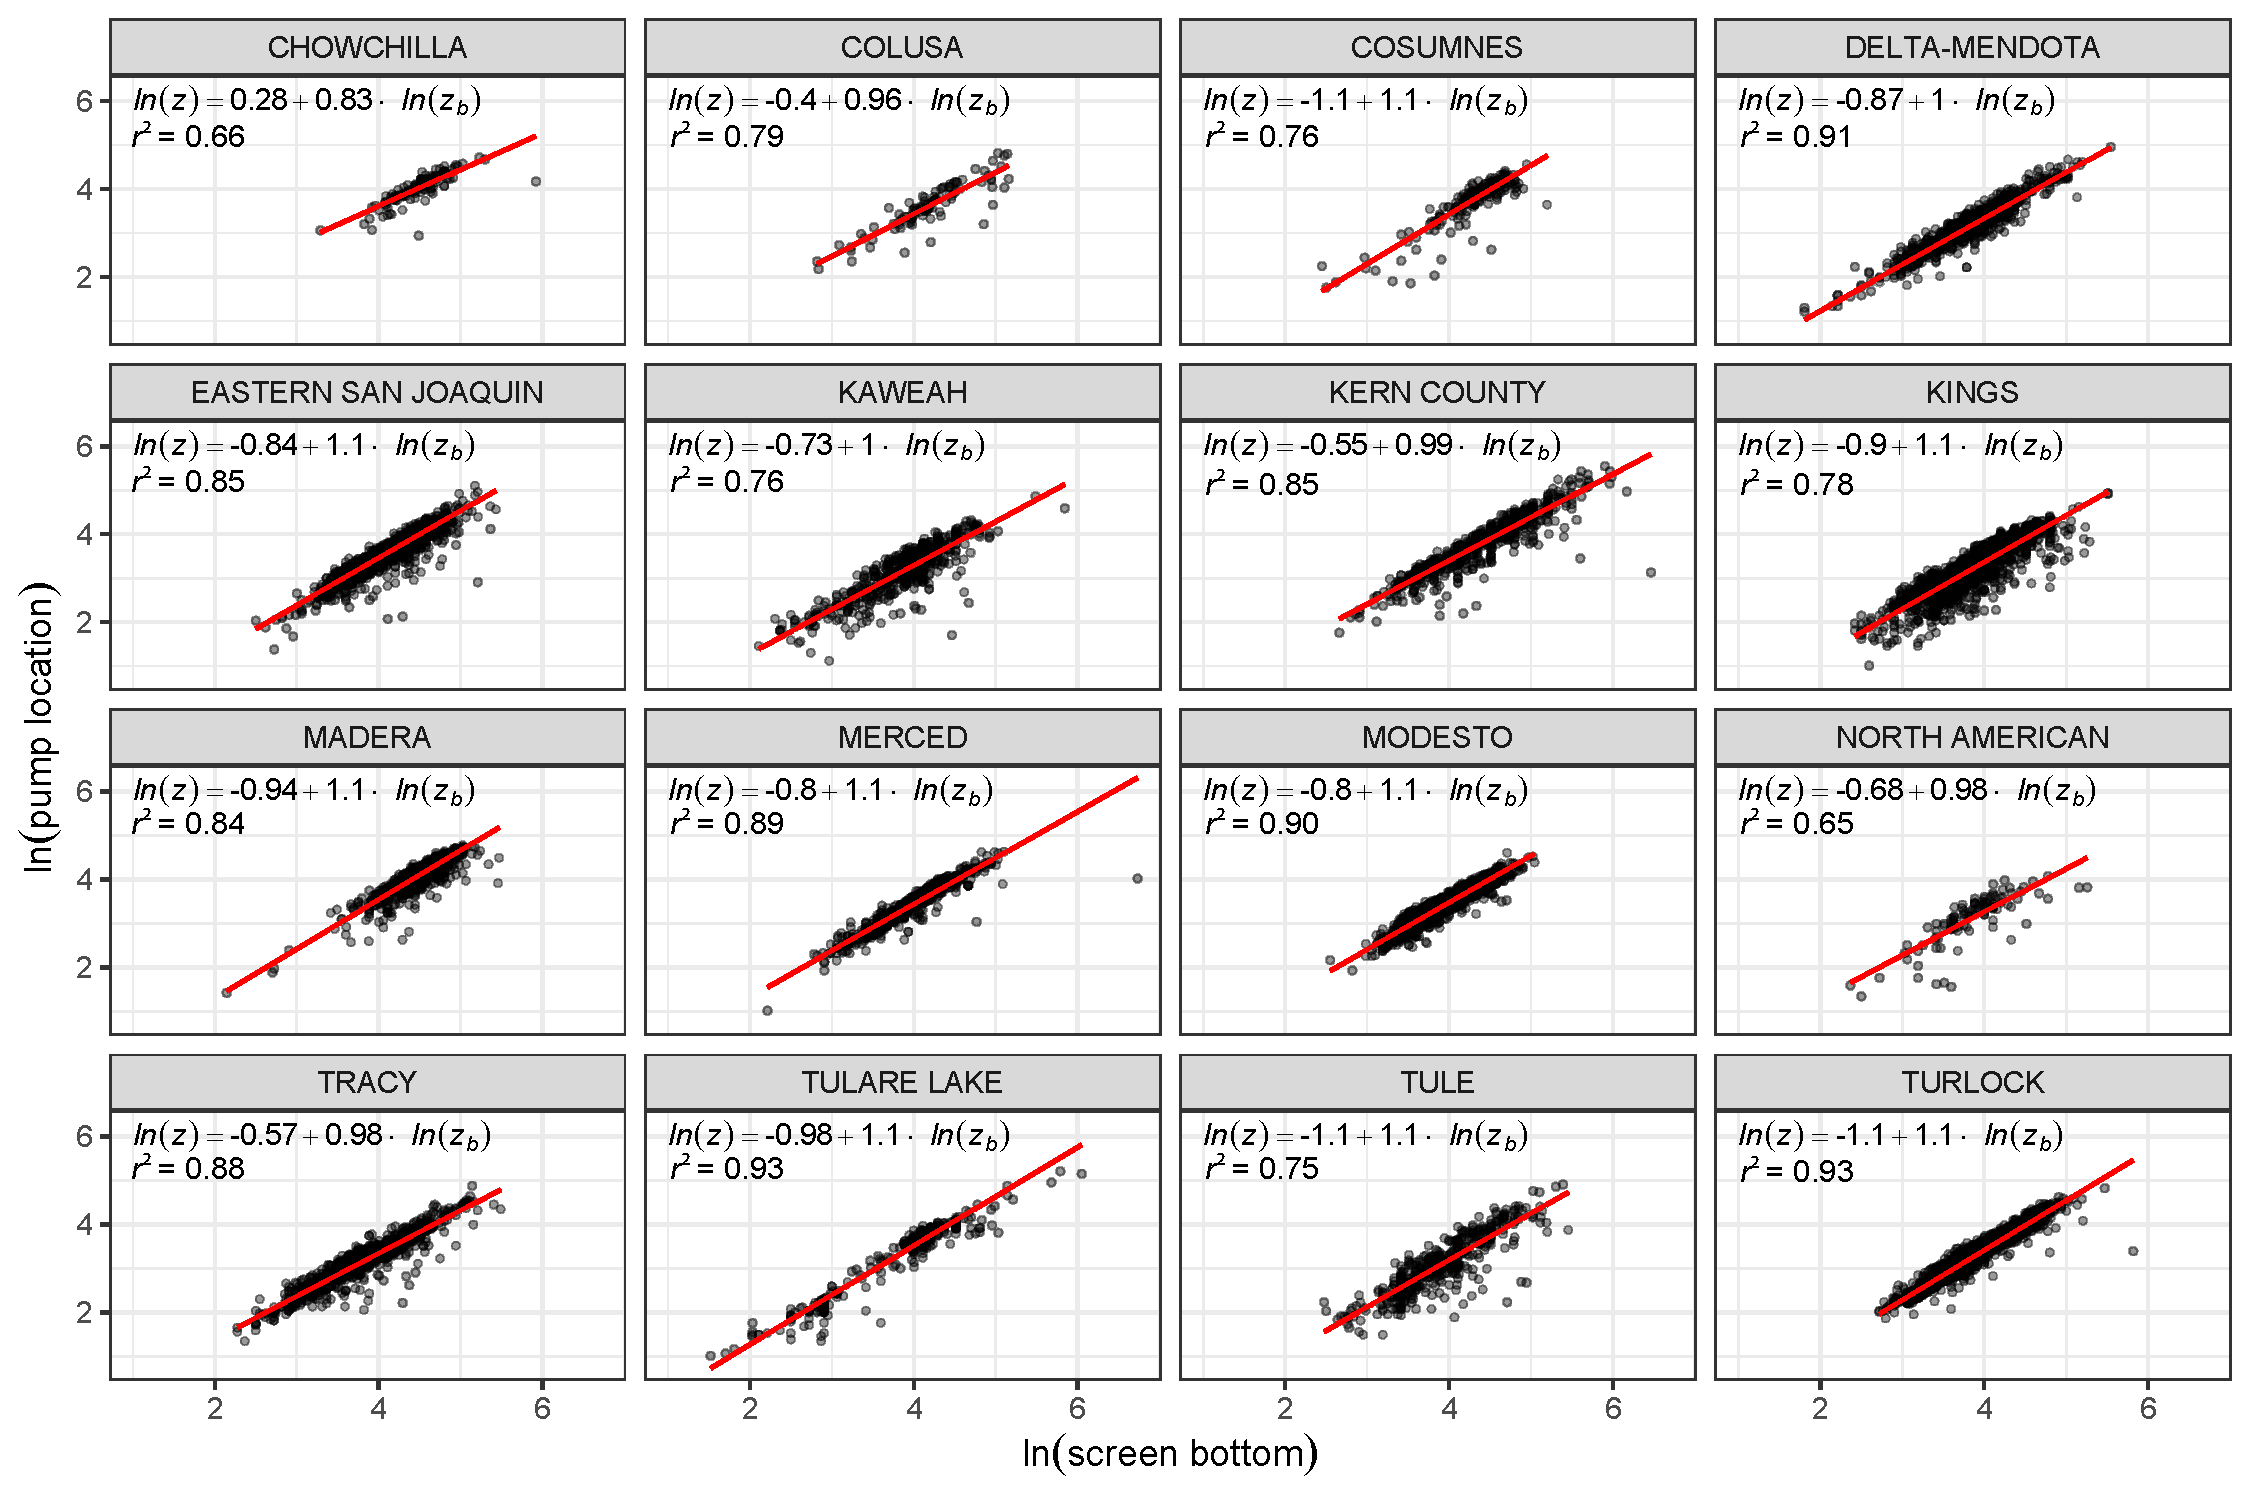
\includegraphics[width=\textwidth]{ch2_appendix_figs/erl_pump_loc_bot_eq.pdf}
	\caption{Relationship between the logarithm of pump depth ($z$), and logarithm of the bottom of the screened interval ($z_{b}$) for a subset of 16 Bulletin 118 subbasins.}
	\label{fig:pump_loc_bottom}
\end{figure}

% map of data dense basins, data poor basins, SBs used to construct linear models, and lines of best fit
%% north_south_impute.png in `08_pump_loc_spatailly_varying.Rmd`
\begin{figure}[ht]
	\includegraphics[width=\textwidth]{ch2_appendix_figs/erl_north_south_impute_eq.pdf}
	\caption{(A) Count of wells per Bulletin 118 subbasin with recorded screen bottom and directly estimable pump depth, further classified into northern and southern subbasins. (B) \& (C) Northern and Southern subbasins used to construct the linear relationships between pump depth and screened interval bottom; the wells within are shown as black points. (D) \& (E) Northern and Southern linear models used to impute pump depth for northern and southern basins with fewer than 75 samples.}
	\label{fig:north_south_impute}
\end{figure}

Pump depth estimates were generally poor in Bulletin 118 subbasins with fewer than 75 wells, such as in the western San Joaquin Valley, and in various subbasins from the Sacramento Valley to the northernmost CV (Figure \ref{fig:north_south_impute}A). To improve pump depth estimates in these regions, we used observations from adjacent subbasins (Figures \ref{fig:north_south_impute}B \&  \ref{fig:north_south_impute}C) to construct linear models relating pump depth and screen depth as described above (Figures \ref{fig:north_south_impute}D \&  \ref{fig:north_south_impute}E).  

The 5 and 95\% confidence intervals for each linear model were calculated via the standard approach \cite{james2013introduction}, and propagated through the model to account for uncertainty in the estimated pump location.   


Distributions of estimated pump intake depth at the DWR Bulletin 118 subbasin level tend to be either normal or left-skewed (Figure \ref{fig:pump_loc_density}), indicating that most pumps are shallow and close to the land surface. The mean estimated pump depth across subbasins ranges from 25.44 $m$ in the North American subbasin to 68.84 $m$ in the Madera subbasin, suggesting that many pumps are, within tens of meters of the land surface. Considering that most groundwater levels are also tens of meters below land surface %(Figure \ref{fig:sp_fall_gwl_2})
, the distance between a particular well's pump and the upper groundwater level may be only a few meters. Consequently, small groundwater level declines of only a few meters during a drought can lead to considerable domestic well failures.  

The strong relationship between the bottom of the screened interval and the estimated pump depth (Figure \ref{fig:pump_loc_bottom}) was a useful approach for imputing missing pump depths. Goodness of fit ($r^2$) for subbasins have a median of 0.84, and range from 0.93 to 0.41. Residual plots were examined and do not exhibit non-constant variance in the error terms or heteroscedasticity, partially because log-transformation dampens the leverage of the few particularly deep wells. Model $\beta_1$ coefficients vary around 1, indicating that in most subbasins, an increase of 1 unit in the screened interval depth corresponds to an increase of 1 unit in the estimated pump depth. As expected, most intercepts ($\beta_0$) are negative, because the bottom of the screened interval is always deeper than the pump depth. Those with positive intercepts (Yolo and Chowchilla) have poor $r^2$ scores compared to other subbasins, attributable partly to a relatively low number of wells.  

Northern basins are smaller in area than southern basins, and also tend to be more sparse in terms of screened interval information. The sparsity of data in some basins motivated the creation of north and south aggregate models (Figures \ref{fig:north_south_impute}A-E) to supplement data-poor basins with fewer than 75 samples. The south and north aggregate models show an $r^2$ of 0.90 and 0.71 respectively. 

Model coefficients, goodness of fit scores, and sample sizes are reported in Table \ref{tab:linear_mod_coef}.


%% Table of linear model coefficients for SBs and north/south aggretate models
% pl_lm.rds and ns_lm.rds in `08_pump_loc_spatially_varying.Rmd`
\begin{table}[ht]
	\centering\footnotesize
	\caption{Linear regression model coefficients, goodness of fit, and sample size for the subset of wells with 75 or more samples.}
	\label{tab:linear_mod_coef}
	\begin{threeparttable}
		
		\begin{tabular}{lcccr}
			\hline
			\hline
			$Subbasin \: Name$ & $\beta_0$ & $\beta_1$ & $r^2$ & $n$ \\
			\hline
			Chowchilla & 0.28 & 0.83 & 0.66 & 133 \\ 
			Colusa & -0.40 & 0.96 & 0.79 &  98 \\ 
			Cosumnes & -1.06 & 1.12 & 0.76 & 260 \\ 
			Delta-Mendota & -0.87 & 1.05 & 0.91 & 1370 \\ 
			Eastern San Joaquin & -0.84 & 1.07 & 0.85 & 2357 \\ 
			Kaweah & -0.73 & 1.00 & 0.76 & 578 \\ 
			Kern & -0.55 & 0.99 & 0.85 & 760 \\ 
			Kings & -0.90 & 1.06 & 0.78 & 2625 \\ 
			Madera & -0.94 & 1.12 & 0.84 & 2300 \\ 
			Merced & -0.80 & 1.06 & 0.89 & 605 \\ 
			Modesto & -0.80 & 1.07 & 0.90 & 1948 \\ 
			North American & -0.68 & 0.98 & 0.65 & 108 \\ 
			Solano & -0.47 & 0.89 & 0.66 &  75 \\ 
			Tracy & -0.57 & 0.98 & 0.88 & 1212 \\ 
			Tulare Lake & -0.98 & 1.12 & 0.93 & 394 \\ 
			Tule & -1.08 & 1.07 & 0.75 & 484 \\ 
			Turlock & -1.13 & 1.13 & 0.93 & 2193 \\ 
			Yolo & 0.80 & 0.65 & 0.41 &  75 \\ 
			North aggregate & -0.97 & 1.06 & 0.71 & 866 \\ 
			South aggregate & -1.11 & 1.09 & 0.90 & 1920 \\ 
			\hline
		\end{tabular}
		
		\begin{tablenotes}[para,flushleft] 
			Logarithm of pump depth $z$ is regressed onto the logarithm of screen bottom elevation, $z_{b}$.
		\end{tablenotes}
	\end{threeparttable}
	
\end{table}



%%%%%%%%%%%%%%%%%%%%%%%%%%%%%%%%
\subsection{Model calibration and performance}
\label{ap_a_calib}

We seek a well failure model that reproduces the observed well failures during 2012-2016 by relating changes in groundwater level to estimated pump locations of wells in the OSWCR database. The developed model may then be used to simulate the impact of future droughts. We perform calibration to minimize error between the observed ($n \! = \! 2,027$) and predicted well failures during the 2012-2016 drought. Model calibration proceeded in three steps. First, groundwater levels across the CV during the 2012-2016 drought were mapped. Second, the spatial units at which the model was calibrated were selected (discussed below). Third, the optimum value of the well retirement age ($t_r$) was determined.

Groundwater levels across the CV were mapped by the interpolation approach described above and in the methods of the paper. In order to calculate groundwater level change over the drought, we set initial and final conditions, and take their difference. Because the observations are not spatially consistent across seasons, we take the mean groundwater level of adjacent seasons to reduce variance in the interpolated surface, and provide a more robust representation of groundwater levels during that time. The initial groundwater level ($g_{t_0}$) is the mean of spring 2011 and spring 2012 measurements, and the final groundwater level is the mean of spring and fall of 2016. The difference of the final and initial conditions defines the groundwater level change over four years of drought from 2012-2016. The upper and lower 2.5 percentiles of the raster (which incidentally coincide with areas of low to zero domestic well occurrence) were assigned to the 2.5 and 97.5 percentiles to control for outliers in the interpolation and improve mapping. The well failure model described in section \ref{ap_a_formal_wf} was then applied.  

%% p_calib_err.png in `06_calibration_herve_alvar_graham_calib_TS.Rmd`
%% GF edit in same file ^^
%% obtain using `lGF_CI.rds` for gw levels with CIs and 
%% `domcv6_mean_gwl_with_beta_GF_CI.rds` for max_gwl during 2012-2016
%% with CIs
\begin{figure}[ht]
	\includegraphics[width=\textwidth]{ch2_appendix_figs/erl_p_calib_err_GF.pdf}
	\caption{(A) Retirement age of domestic wells and associated SSE in the calibration spatial units. Low retirement ages remove too many wells from the model, resulting in unrealistically low SSE compared to a validation set. (B) Retirement age of domestic wells and associated count of failing wells during the 2012-2016 drought. The horizontal dashed black line shows the number of observed failing wells during the drought, constraining the feasible solution space to retirement ages of 25 years or greater. The red dot indicates the most reasonable model that balances low SSE, acceptable retirement age (28 years), and a compensation for well failure under-reporting. Error bars show the 5 and 95\% confidence intervals of predicted well failures, computed by propagating uncertainty in pump location estimation and groundwater level estimation through the model.}
	\label{fig:calib_err}
\end{figure}

One free parameter, the well retirement age ($t_r$) controls the number of wells active at time zero and thus the accuracy of the model. The optimum retirement age was determined by minimizing the sum of squared error (SSE) between the observed and predicted proportion of well failure across all calibration units (Figure \ref{fig:calib_err}). Retirement ages from 20 to 40 years were tested, with the assumption that the true retirement age was within this range. SSE is calculated for the observed well failure \textit{proportion} rather than the observed well failure \textit{count}, because proportions are normalized by the total number of wells in each spatial unit. Thus, the error term weights all calibration units equally, and the calibration units with unusually low or high well counts do not exert excessive leverage.  


Three-by-three blocks of PLSS townships (henceforth called aggregate-townships; length = 28.97 $km$, area = 839.16 $km^2$) were selected as the spatial units for calibration for two main reasons. First, since well failure reporting occurs at a county-level, calibration units must be at least this size, which the aggregate-township level achieves. Second, townships are meaningful units of spatial organization to planners and managers. We experimented with smaller calibration scales, such as the PLSS section (length = 1.61 $km$, area = 2.59 $km^2$), and PLSS township (length = 9.67 $km$, area = 93.24 $km^2$). However, small calibration spatial units suffer from high variance in prediction error: some spatial units show very low prediction error (e.g.- zero observed and zero predicted failures), while others show very high prediction error (e.g. - when a large difference between observed and predicted well failures exists). These differences are attributable to uncertainty in well failure reporting, well completion reporting, and groundwater level. A coarser calibration resolution at the aggregate-township (length = 28.97 $km$, area = 839.16 $km^2$) is less likely to contain spatial units with zero observations, and also averages the variance of observed failures at a larger scale, thus permitting spatially-explicit model validation at a coarser resolution. Small spatial units along the alluvial boundary edge less than 600 $km^2$ were removed in order to focus the calibration in regions representative of high well density. 

To further control for uncertainty in the voluntary well failure reporting data, which we expect is more likely to be under-reported than not, only calibration units with observed failure ratios between the 25\% and 95\% percentiles were considered. Like well failure reporting, OSWCR reporting is also likely to under-count total domestic wells, thus only calibration units with well counts between the 25\% and 95\% percentiles were considered. Lastly, only aggregate-townships with at least 20 observed well failures were considered in the calibration. We select this threshold because it represents approximately 1\% of the roughly 2,000 observed well failures during the 2012-2016 drought. Eleven final aggregate-townships were selected to perform the calibration.    


The well retirement age parameter ($t_r = 28$ years) led to the most reasonable model that balanced low SSE, and agreed with the mean retirement age for domestic wells in the CV found by \cite{Gailey2019}. The 2,027 observed failures during the 2012-2016 drought imposes a hard constraint on feasible retirement ages equal to or greater than 25 years, because under this value, the predicted well failure count is less than the observed well failure count (Figure \ref{fig:calib_err}B). Low retirement ages (20-22 yrs) removed too many wells from the model, resulting in unrealistically low well failure count, (Figure \ref{fig:calib_err}A), and high retirement ages (37-40 yrs) left too many wells in the model, which led to high SSE and an unrealistically large number of well failures (greater than observed during the 2012-2016 drought). 

%% calibration_pred_obs_line.ai
%% calib.pdf in `06_calibration_herve_alvar_graham_calib_TS.Rmd`
%% GF edit in ^^ Rmd file and .ai file at calibration_pred_obs_line.ai
\begin{figure}[H]
	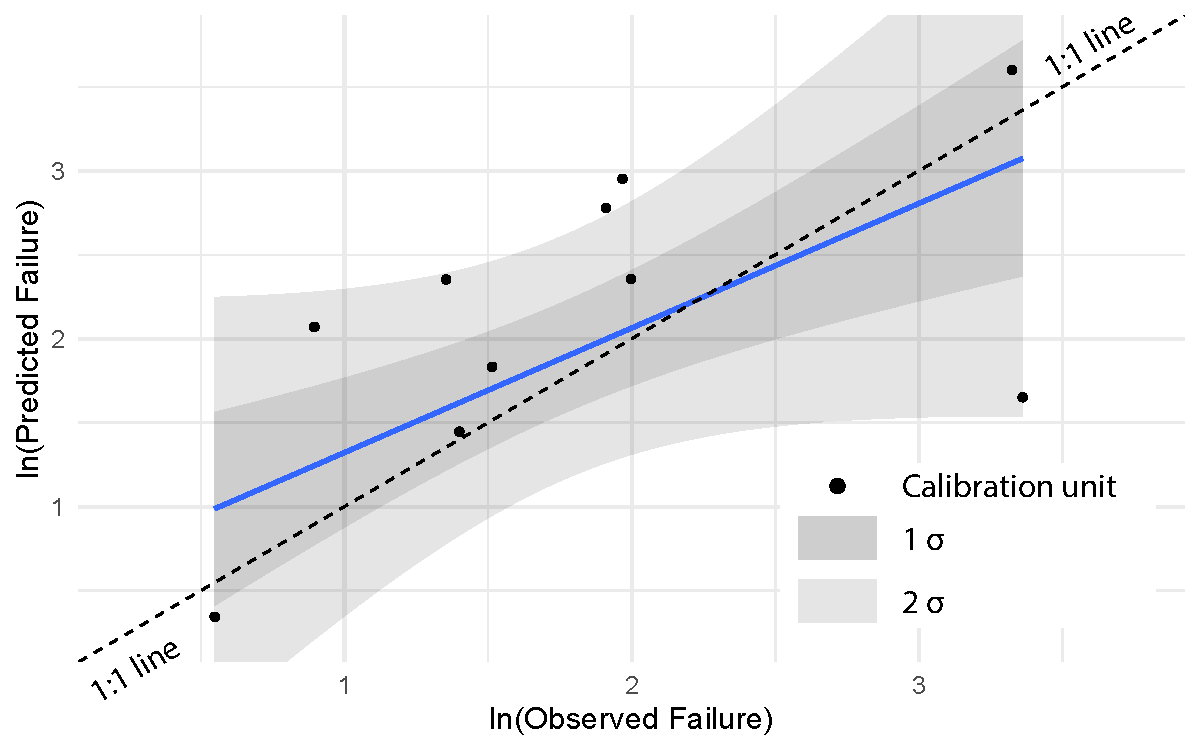
\includegraphics[width=\textwidth]{ch2_appendix_figs/erl_calibration_pred_obs_line_GF.pdf}
	\caption{Predicted vs. observed log failure ratio for the 11 calibration spatial units. }
	\label{fig:calib_line}
\end{figure}

The fit between observed and predicted calibration units suggests relatively high local-scale error, with four calibration units falling more than 2 standard deviations from the least squares line through the observed and predicted scatter plot (Figure \ref{fig:calib_line}). These discrepancies are the product of uncertainty in well failure reporting, well completion reporting, groundwater level, and model formulation. As the failure model is subject to local error it is best interpreted as a regional-scale domestic well failure estimate. 

\clearpage



\begin{table}[ht]
	\centering\footnotesize
	\caption{Domestic well failure counts under different groundwater management regimes (Sustainable, Glide path, and Business as usual).}
	\label{tab:dom_failures}
	\begin{threeparttable}
	
		
		\begin{tabular}{lrrr}

			\hline
			\hline
			
			\textbf{scenario} & \textbf{mean failure count} & \textbf{5\% CI failure count} & \textbf{95\% CI failure count} \\
			
			\hline
			
			\multicolumn{4}{l}{\textbf{\textit{Sustainable}}}\\
			\hspace{1em}1998-2017 & 1516 & 1248 & 1809\\
			\hspace{1em}2003-2017 & 2000 & 1619 & 2412\\
			\hspace{1em}2008-2017 & 2513 & 2200 & 2914\\
			
			\hline
			\multicolumn{4}{l}{\textbf{\textit{Glide path}}}\\
			\hspace{1em}1998-2017 & 3677 & 3359 & 4039\\
			\hspace{1em}2003-2017 & 4929 & 4509 & 5361\\
			\hspace{1em}2008-2017 & 6943 & 6501 & 7417\\
			
			\hline
			\multicolumn{4}{l}{\textbf{\textit{Business as usual}}}\\
			\hspace{1em}1998-2017 & 5966 & 5650 & 6293\\
			\hspace{1em}2003-2017 & 7677 & 7239 & 8092\\
			\hspace{1em}2008-2017 & 10466 & 10087 & 10885\\
			\hline
			
		\end{tabular}
		
		\begin{tablenotes}[para,flushleft] 
		
			The mean failure count corresponds to the number of wells failing when the mean pump depth is used. Well failures at the 5\% confidence interval (CI) and 95\% CI correspond to uncertainty in the estimated pump location. Hydrologic uncertainty in groundwater level is accounted for by considering three different linear approximations of groundwater level decline, beginning in 1998, 2003, and 2008.
		\end{tablenotes}
	\end{threeparttable}
\end{table}

\clearpage



%--------------------------------------------------------%
% Acknowledgements
%--------------------------------------------------------%
\section{Acknowledgments}
We thank the Governor's Office of Planning and Research and the California Department of Water Resources for their assistance in acquiring domestic well failure, and well completion report data. Thomas Harter, Darcy Bostic, and Nisha Marwaha provided modeling advice and assistance. The West Big Data Hub has helped disseminate this research. Financial support was provided by the National Science Foundation (NSF) Climate Change, Water, and Society (CCWAS) Integrated Graduate Education and Research Traineeship (IGERT) program at the University of California, Davis (http://ccwas.ucdavis.edu, DGE-10693333), and the University of California Water (UC Water) Security and Sustainability Research Initiative.


%--------------------------------------------------------%
% Data
%--------------------------------------------------------%
\section{Data availability}
The data that support the findings of this study are openly available. These data\citep{Pauloo2019} do not include observed well failure data \citep{observedDW}, which are confidential and must be obtained by contacting the California Department of Water Resources. 

\clearpage
%\printbibliography[heading=bibliography]

% chapter 3
%\chapter{Real Title Here}
%
%This is an example for a chapter, additional chapter can be added in the skeleton-thesis
%To generate the final document run latex, build and quick build commands on the skeleton-thesis file not this one.
%This is chapter 2, the default skeleton thesis expects 2 chapters
\chapter[Sensitivity of Hydrologic and Geologic Parameters on Recharge Processes in a Highly-Heterogeneous, Semi-Confined Aquifer System]{Sensitivity of Hydrologic and Geologic Parameters on Recharge Processes in a Highly-Heterogeneous, Semi-Confined Aquifer System.\footnote[1]{This chapter is in review at \textit{Hydrology and Earth System Sciences (HESS)}: Maples, S. R., Foglia, L, Fogg G. E., \& Maxwell, R. M. ``Sensitivity of Hydrologic and Geologic Parameters on Recharge Processes in a Highly-Heterogeneous, Semi-Confined Aquifer System''. (Preprint doi:10.5194/hess-2019-412)}}

%~~~~~~~~~~~~~~~~~ ABSTRACT ~~~~~~~~~~~~~~~~~
\section{Abstract}

\noindent Increasing reliance on groundwater resources has been observed worldwide during the past 50–70 years and has led to unsustainable groundwater abstraction in many regions, especially in semi-arid and arid alluvial groundwater basins. Managed aquifer recharge (MAR) has been promoted to replenish overdrafted groundwater basins and augment surface water supply. However, MAR feasibility in alluvial groundwater basins is complicated by complex geologic architecture that typically includes laterally-continuous, fine-texture confining units that can impede both recharge rates and regional propagation of increases in hydraulic head. Greater feasibility of MAR hinges on identifying locations where rapid, high-volume recharge that provides regional increases in pressure head are possible, but relatively little research has evaluated the factors that control MAR feasibility in alluvial groundwater basins. Here, we combine a transition probability Markov-chain geostatistical model of the subsurface geologic heterogeneity of the east side of the northern Central Valley, California, with the 3D, variably-saturated water flow code, ParFlow, to explore the variability of MAR feasibility in this region. We use a combination of computationally-efficient local and global sensitivity analyses to evaluate the relative importance of factors that contribute to MAR feasibility. A novel proxy parameter approach was used to describe the configuration and proportions of subsurface hydrofacies and water table depth for sensitivity analyses, and results suggest that recharge potential is relatively more sensitive to the variability of this proxy parameter than to the variablity of individual hydrofacies hydraulic properties. Results demonstrate that large variability of MAR feasibility is typical for alluvial aquifer systems and that outsized recharge rates are possible in select locations where interconnected, coarse-texture hydrofacies occur.

%~~~~~~~~~~~~~~~~~ INTRODUCTION ~~~~~~~~~~~~~~~~~
%%%\clearpage
\section{Introduction} \label{sec:intro} 


Geologic heterogeneity strongly affects both the movement of water in the subsurface and the exchange of water between subsurface and surface stores; however, rarely are enough data available to explicitly represent heterogeneous geologic features in groundwater models \citep{koltermann1996heterogeneity,deMarsily2005heterogeneity}. Instead, models typically simplify and/or upscale heterogeneity to represent subsurface flows for purposes of regional-scale water resources management \citep[e.g.,][]{fogg1986groundwater,phillips1991calibration}. Upscaling methods have been the focus of numerous studies \citep[e.g.,][]{renard1997calculating, fogg2000connected, neuman2003multifaceted, fleckenstein2008efficient}, and coarse-resolution models with upscaled (i.e., effective) hydrologic properties are often adequate for regional-scale flow studies, but typically lack enough detail to reliably capture some phenomena, like recharge and transport processes, that are strongly influenced by geologic heterogeneity. 

To represent the influence of geologic heterogeneity on flow and transport phenomena, many approaches have relied on stochastic methods, like transition probability based indicator geostatistics which can represent heterogeneous features while honoring measured data \citep{carle1996tprogs,weissmann1999multi,weissmann1999three}. These approaches represent geologic heterogeneity with hydrogeologic facies categories, each of which is assigned effective values or probability densities for estimates of hydraulic properties. By categorizing facies according to depositional environment rather than texture alone, the predictable geometries (i.e., facies mean lengths, proportions, and juxtapositions) of these features can be more accurately represented with sparse data. Studies that rely on these methods show strong influence of subsurface heterogeneity on groundwater/surface-water interactions and recharge processes \citep{LeeSiYong2004thesis,fleckenstein2006river,engdahl2010evaluation,liu2014thesis}, including managed aquifer recharge (MAR) \citep{maples_2019}, especially for instances when the mean lengths and proportions of high-permeability facies allow for percolation, i.e., formation of connected networks \citep{fogg2000connected,harter2005finite}.

Accurately assigning aquifer properties in models can be a challenge because they are scale dependent attributes that are challenging to measure and can vary over many orders of magnitude in typical aquifer systems \citep[e.g.,][]{sudicky1986natural,gelhar1992critical,weissmann1999multi}. While aquifer tests can accurately constrain estimates of hydraulic conductivity ($K$) for high-permeability facies, they are typically unreliable for estimating $K$ of low-permeability (i.e.,  aquitard) facies \citep{fogg1986groundwater,fogg1998geologically}, which have been shown to influence pumping response \citep{fogg2000connected} and be important for accommodating recharge \citep{maples_2019}.
Reconciling typically sparse measurements of aquifer properties from aquifer tests with the representation of effective values in models is often the source of large uncertainty because parameterization of the properties in models is scale dependent \citep{sudicky1991contaminant}, and is typically achieved through model calibration.

The contaminant transport community has long recognized the strong influence of $K$ scaling and geologic heterogeneity on transport processes \citep[e.g.,][]{gelhar1992critical,sudicky1991contaminant,koltermann1996heterogeneity}, and recent work has extended these concepts to assess their role on runoff generation, evapotranspiration (ET), and feedbacks between subsurface and land-surface water in integrated hydrologic models \citep{srivastava2014insights,gilbert2016global,foster2019sensitivity}, but relatively little research has focused on the influence these factors for MAR processes specifically. Recent work has highlighted the importance of connected networks of high-$K$ facies for MAR \citep{maples_2019}, but to our knowledge the sensitivity of MAR processes to these heterogeneous geologic features as compared to other uncertain hydraulic properties has not been formally evaluated. 

Sensitivity analyses are a fundamental diagnostic tool to provide insight into the relative importance of the parameterization of aquifer properties among other inputs to complex hydrologic models \citep{saltelli2004sensitivity}. Sensitivity analyses can be broadly categorized as local or global methods, where local methods provide sensitivity evaluation at a single location in the parameter space \citep{hill2007effective}, while global approaches explore sensitivities throughout a multi-dimensional parameter space \citep{saltelli2008global}. Many studies have shown the diagnostic utility of local approaches \citep[e.g.,][]{foglia2009sensitivity}; however, local approaches are generally less robust than global approaches, especially for non-linear models \citep{saltelli2008global}. On the other hand, global methods are typically orders of magnitude more computationally expensive than local approaches.

Here, we simulate variably-saturated MAR dynamics in a highly-resolved representation of complex subsurface geologic heterogeneity of a clastic, unconsolidated sedimentary aquifer system that includes both interconnected, high-$K$ sand and gravel deposits intermingled with silt- and clay-dominated sediments. We use a combination of local and global sensitivity analyses to provide insight into the relative importance of the subsurface geologic facies configuration and parameterization of subsurface hydraulic properties on MAR processes. This work provides insight into important factors to consider when investigating potential MAR sites and also highlights the utility of a combination of computationally-frugal local and global sensitivity analyses for computationally-intensive hydrologic models.


%~~~~~~~~~~~~~~~~~ MATERIALS AND METHODS ~~~~~~~~~~~~~~~~~
%~~~~~~~~~~~~~~~~~ SUBSECTION boundary conditions ~~~~~~~~~~~~~~~~~
\section{Materials and Methods} \label{sec:MM}
\subsection{Local Hydrogeology and Domain Extent} \label{ssec:MM_hydrogeology}
The model domain covers about 1640 km\textsuperscript{2} of the east side of the northern Central Valley, California, near the convergence of the lower portions of the American and Cosumnes Rivers with the Sacramento River (Fig. \ref{fig:domain}). The domain comprises a low-angle alluvial fan complex that is typical of the Central Valley where previous studies have documented the presence of  deposits that are favorable for recharge \citep{shlemon1967landform,meirovitz2010thesis}, including massive, interconnected, highly-permeable sand and gravel deposits known as incised valley fill [IVF, \citep{weissmann2004influence, weissmann2005factors}] that form from  river incision and deposition events during cyclic Plio-Pleistocene Sierra Nevada glaciation. In places, multiple IVF deposits have been shown to overlap and interconnect from land surface into the deeper aquifer system, forming massive, coarse-texture, relatively high-permeability pathways for recharge that bypass local, otherwise laterally-extensive confining units. These features have been shown to accommodate recharge volumes that are orders of magnitude greater than would be possible over the rest of the landscape \citep{maples_2019}. Other studies have shown that IVF features likely occur on river fans throughout the Central Valley \citep{weissmann2005factors}, and in similar glacially-influenced rivers \citep{pierce1983pleistocene} but are still largely undocumented.

%% FIGURE 1
\begin{figure*}[t]
\centering
\includegraphics[width=16.5cm]{ch2_figs/Fig_01_080619_HESS.pdf}
\caption{Location of model domain in the in the Central Valley aquifer system in California, and (a) inset of the uppermost layer of the model hydrofacies overlain over aerial imagery of the Central Valley and local river systems.}
\label{fig:domain}
\end{figure*}

The local hydrostratigraphy of the area is described in detail by \cite{meirovitz2010thesis} and \cite{maples_2019}. In general, the two major rivers intersecting the domain, the American and Cosumnes Rivers, have markedly different depositional characteristics. The American River drains a large ($>$4000 km\textsuperscript{2}), high-elevation catchment that extends to the Sierra Nevada crest [$>$3000 m above mean sea level (amsl)]. As a result, the American River was greatly influenced by cyclic plio-pleistocene glaciation that deposited IVF in the domain area. Conversely, the Cosumnes River catchment is smaller (900  km\textsuperscript{2}) and lower in elevation. As a result, deposits from the Cosumnes River do not contain IVF and are typically finer in texture. In some locations in the domain area, Quaternary and Holocene channel avulsion of the American River resulted in a more southwest course that intersects the current path of the Cosumnes river, creating complex overlapping stratigraphy in that area. Cross-cutting IVF and overlapping paleochannel networks in the domain area result in an aquifer system that is typically unconfined (and sometimes perched) or semi-confined at shallow depths and increasingly confined with depth  \citep{fleckenstein2006river,liu2014thesis,niswonger2008influence}. Groundwater pumping in the region typically occurs at depths $>$30 m in the deeper semi-confined or confined portion of the aquifer system \citep{liu2014thesis}.

%~~~~~~~~~~~~~~~~~ SUBSECTION hydrofacies model development ~~~~~~~~~~~~~~~~~
\subsection{Hydrofacies Model Development} \label{ssec:MM_tprogs_model}
Transition probability Markov-chain geostatistics (TPROGS) \citep{carle1996tprogs,carle1997modeling,carle1999t}, was used to simulate the subsurface distribution of hydrofacies in the domain area (Fig. \ref{fig:domain_3d}). Model development is described in detail by \cite{meirovitz2010thesis} and \cite{maples_2019}. Roughly 1200 well logs, soil surveys, geologic cross-sections and mapped paleochannels were used as conditioning data for the TPROGS model. Geologic data were binned into four textural categories: gravel, sand, muddy sand, and mud (undifferentiated silt and/or clay) [Table \ref{table:textural_characteristics} \citep{fleckenstein2004managing,meirovitz2010thesis}]. "Mud" refers to silt and clay undifferentiated, because most of the subsurface data available  only identify the fine-grained sediments and are not sufficiently detailed to distinguish silt from clay. From these data the proportions for each facies were calculated directly. Through geologic analysis of the data, additional parameters were estimated describing the mean lengths of each hydrofacies along the principal directions and the embedded transition probabilities to represent cross-correlation between different facies. Because the depositional characteristics of the American and Cosumnes fans were markedly different, individual models of each were produced and subsequently combined  by  \cite{meirovitz2010thesis}. 

%% FIGURE 2
\begin{figure}[t]
\centering
\includegraphics[width=9.0cm]{ch2_figs/Fig_02_080619_HESS.pdf}
\caption{Three-dimensional representation of the model domain.}
\label{fig:domain_3d}
\end{figure}

%% TABLE 1
\input{ch2_tables/Table_1_textural_characteristics.tex}

The model uses an orthogonal grid geometry with 181 $\times$ 227 $\times$ 265 cells in the x-, y-, and z- directions, respectively. The x- and y- directions of the grid were rotated 17.85 degrees counterclockwise from the cardinal directions, and the z-direction was oriented vertically. Cell sizes were 200 $\times$ 200 $\times$ 1 m. The total domain size is 36.2 $\times$ 45.4 $\times$ 0.265 km, in the x-, y- and z-directions, respectively. Cells located above land surface were designated as inactive in the model, resulting in about 7.3 million active cells in the domain area. 

%~~~~~~~~~~~~~~~~~ SUBSECTION hydrologic model development ~~~~~~~~~~~~~~~~~
%~~~~~~~~~~~~~~~~~ sub-subsection governing eqns ~~~~~~~~~~~~~~~~~
\subsection{Hydrologic Model Development} \label{ssec:MM_parflow_model}
\subsubsection{Governing Equations} \label{sssec:gov_eqn}
Three-dimensional, variably-saturated water flow was simulated with the hydrologic modeling code, ParFlow \citep{ashby1996parallel,jones2001newton,kollet2006integrated}, which couples surface and subsurface flow with the 2-D diffusive or kinematic wave equation, and solves the 3-D mixed form of Richards' Equation for variably-saturated subsurface flow: 

\begin{equation}
S_s S_w(h) \frac{\partial h}{\partial t} + \phi \frac{\partial S_w(h)}{\partial t} 
= \nabla \cdot \textbf{q}+ q_r(x,z)
\label{richards_eqn1}
\end{equation}
\noindent where
\begin{equation}
\textbf{q}
= \phi S_w (h) \textbf{v}
= -\textbf{K}_s (x) k_r (h) \nabla (h+z)
\label{richards_eqn2}
\end{equation}

\noindent In these equations $S_s$ is specific storage [L\textsuperscript{$-$1}], $S_w$ is relative saturation [$-$], $h$ is pressure head [L], $t$ is time [T], $\phi$ is porosity [$-$], $\textbf{q}$ is Darcy flux [L T\textsuperscript{$-$1}], $q_r$ is a source/sink term [T\textsuperscript{$-$1}], $z$ is elevation [L], $\textbf{v}$ is the subsurface flow veolicty [L T\textsuperscript{$-$1}], $\textbf{K}_s(\textbf{x})$ is the saturated hydraulic conductivity tensor [L T\textsuperscript{$-$1}], and $k_r$ is relative permeability [$-$]. The van Genuchten relations \citep{vangenuchten1980} describe $S_w$ and $k_r$ as a function of $h$ in the unsaturated zone, with parameters for air entry pressure $\alpha$ [L\textsuperscript{$-$1}], pore size distribution $n$ [$-$], and residual saturation $S_{res}$ [$-$].

%~~~~~~~~~~~~~~~~~ sub-subsection boundary conditions ~~~~~~~~~~~~~~~~~
\subsubsection{Boundary Conditions} \label{ssec:MM_BCs}
Model boundary conditions are discussed in greater detail in \cite{liu2014thesis} and \cite{maples_2019}. The locations of domain boundaries were chosen to simplify the assignment of boundary conditions for the flow model. The eastern boundary roughly coincides with the Sierra Nevada foothills, and the northern, southern, and western boundaries roughly coincide with local surface water bodies (Fig. \ref{fig:domain}). A specified head boundary condition was applied for the eastern boundary to coincide with the local groundwater head distribution estimated from local monitoring well data \citep{liu2014thesis}. A general head boundary of 0 m amsl was set 1 km beyond the western boundary to approximate the Sacramento River and Sacramento-San Joaquin Delta along the northwestern, and southwestern portions of the western boundary, respectively. No-flow boundary conditions were applied along northern, southern, and bottom boundaries because the regional groundwater flow direction is generally from east to west. Model spin up and recharge simulations used combinations of specified-flux and specified-head upper boundary conditions and are described in greater detail in subsequent sections.

%~~~~~~~~~~~~~~~~~ sub-subsection model spinup ~~~~~~~~~~~~~~~~~
\subsubsection{Model Spinup and Calibration} \label{sssec:MM_spinup}

Model spinup and calibration are described in greater detail in \cite{liu2014thesis} and \cite{maples_2019}. To summarize, a 16-yr. simulation period was used to bring the simulated hydrology into dynamic equilibrium. This period represents 1970–1985, which includes both a wet (1984) and dry (1977) year. Water budget components, including groundwater discharge, recharge and boundary flows along with facies hydraulic properties were estimated and adjusted manually to simulate a realistic water budget, water table configuration, and vertical hydraulic gradients during the calibration process. An initial potentiometric surface was specified using interpolated groundwater level data. Monthly estimated urban and agricultural groundwater pumping rates were applied as specified fluxes representing wells screened in lower portions of the domain that coincide with typical screened intervals of municipal and agricultural pumping wells in the region. Dominant sources of recharge for the region include stream recharge from the American River, Cosumnes River, and Deer Creek, as well as deep percolation from agricultural and urban return flows. Weekly estimates of spatially-distributed river stage for the streams were applied as specified heads along coincident land surface cells. Monthly estimates of urban and agricultural recharge volumes were applied as a specified-flux boundary condition across the top of the domain to simulate deep percolation of agricultural and urban return flows and to equilibrate soil moisture conditions in the near-surface UZ cells. Hydraulic properties for each facies category were calibrated manually (Table \ref{table:facies_properties}) and are consistent with the range of literature values for the Central Valley, California, and for similar alluvial systems \citep{anderson2015applied,botros2009spatial,fleckenstein2004managing,frei2009patterns,maserjian1993hydrogeologic,niswonger2008influence,sager2012effects}.

%% TABLE 2
\input{ch2_tables/Table_2_parameter_ranges.tex}

All simulations were performed using the Cheyenne high-performance cluster at NCAR's Computational and Information Systems Laboratory (doi:10.5065/D6RX99HX). The numerical problem was distributed on 540 cores for each simulation. Approximately 450 model evaluations were required for the exploratory simulations, local sensitivity analyses, and global sensitivity analyses described in subsequent sections, which required approximately 400,000 core-hours of computing time in total. The large computational expense for each simulation (890 core-hours per simulation, on average) required that computationally resources be allocated efficiently. 

%~~~~~~~~~~~~~~~~~ SUBSECTION Exploratory Simulations ~~~~~~~~~~~~~~~~~
%~~~~~~~~~~~~~~~~~ sub-subsection site selection ~~~~~~~~~~~~~~~~~
\subsection{Exploratory Simulations} \label{ssec:MM_exploratory_sims}
\subsubsection{Site Selection} \label{sssec:MM_site_selection}
One hundred 1 km\textsuperscript{2} recharge sites, each encompassing 25 upper-boundary cells, were chosen to approximate hypothetical MAR infiltration basins (Fig. \ref{fig:domain_characteristics}a). Each site was randomly selected from a 910 km\textsuperscript{2} region within the domain that excluded locations within 5 km of lateral domain boundaries to minimize the influence of boundary conditions. The 100 exploratory sites encompass roughly 6\% of the total domain area, which was deemed sufficient to sample the variability of site characteristics observed across the domain. The size of each site was chosen to reflect a regional-scale MAR site, which range from large networks of basins $>$25 km\textsuperscript{2} in size \citep[e.g.,][]{kernFAQ} to individual infiltration basins over several hectares or smaller \citep[e.g.,][]{beganskas2017coupling} in California.

%% FIGURE 3
\begin{figure*}[t]
\centering
\includegraphics[width=16.5cm]{ch2_figs/Fig_03_080619_HESS.pdf}
\caption{Plan view of the model domain, where (a) $K\textsubscript{sat}$ of the uppermost model layer (i.e., the surface expression) at all 41,087 x,y cell locations is overlaid with the locations of 100 randomly-sampled 1-km\textsuperscript{2} exploratory recharge sites (red squares) randomly chosen from 910 potential locations. (b) Arithmetic, (c) geometric, and (d) harmonic mean of vertical $K\textsubscript{sat}$ for unsaturated zone (UZ) facies (i.e., $K\textsubscript{geom}$, $K\textsubscript{arith}$, $K\textsubscript{harm}$, respectively) are shown for all x,y cell locations, along with (e) coarse-texture (gravel and sand) fraction of UZ facies ($UZ\textsubscript{coarse}$), (f) simulated initial depth-to-water ($WTD$), and (g) $K\textsubscript{geom}$ multiplied by $WTD$ ($K\textsubscript{geom} \times WTD$).}
\label{fig:domain_characteristics}
\end{figure*}
%~~~~~~~~~~~~~~~~~ sub-subsection site characteristics ~~~~~~~~~~~~~~~~~
\subsubsection{Site Characteristics} \label{ssec:MM_site_char}

\cite{maples_2019} highlighted that the (1) relative proportions, and degree of vertical interconnection, of coarse-texture facies (sand and gravel) and (2) the unsaturated-zone thickness beneath recharge sites are important factors for recharge feasibility. In this study, we sought to develop site characteristics to describe recharge feasibility at the 100 exploratory sites across the domain. First, we use a heuristic approach of simple averages to bound the expected range of effective (i.e., upscaled) vertical $K\textsubscript{S}$ at all 41,087 x,y cell locations across the domain, where the arithmetic and harmonic mean ($K\textsubscript{arith}$ and $K\textsubscript{harm}$) are the upper and lower bounds, respectively, and the geometric mean ($K\textsubscript{geom}$) is an intermediate value. $K\textsubscript{arith}$ and $K\textsubscript{harm}$ are typically used to approximate groundwater flow parallel and perpendicular to layering, respectively, in anisotropic systems \citep{freeze1979groundwater}. This concept has been generally been extended to variably-saturated flow \citep{mualem1984anisotropy, yeh1985stochastic1, yeh1985stochastic3, assouline2006anisotropy}. \cite{fogg2000connected} showed that vertical groundwater flow in systems with vertically-connected networks of permeable facies tends toward values between $K\textsubscript{arith}$ and $K\textsubscript{geom}$. For each x,y cell location across the domain, $K\textsubscript{arith}$, $K\textsubscript{geom}$, and $K\textsubscript{harm}$ are given as:

\begin{equation}
K\textsubscript{arith} = \frac{K\textsubscript{1}+K\textsubscript{2}+...+K\textsubscript{n}}{n}
\label{Karith_eqn}
\end{equation}

\begin{equation}
K\textsubscript{geom} = {\sqrt[n]{K\textsubscript{1}\times K\textsubscript{2}\times ...\times K\textsubscript{n}}}
\label{Kgeom_eqn}
\end{equation}

\begin{equation}
K\textsubscript{harm} = \frac{n}{\frac{1}{K\textsubscript{1}}+\frac{1}{K\textsubscript{2}}+...+\frac{1}{K\textsubscript{n}}}
\label{Kharm_eqn}
\end{equation}

\noindent where $n$ is the number of vertically-coincident cells from the land surface to the initial water table depth (i.e., the unsaturated-zone cells) for each x,y cell location. In addition, the initial unsaturated-zone thickness ($WTD$) and proportion of coarse-texture sand and gravel unsaturated-zone facies ($UZ\textsubscript{coarse}$) at each x,y cell location across the domain were included as metrics. Additional metrics were developed for each x,y cell location by combining individual metrics, i.e., $WTD$ was used as a multiplier for $K\textsubscript{arith}$, $K\textsubscript{geom}$, $K\textsubscript{harm}$, $Surf\textsubscript{coarse}$, and $UZ\textsubscript{coarse}$. Spatial distributions of select metrics at all x,y cell locations are shown in Fig. \ref{fig:domain_characteristics}.

Site characteristics were calculated for the 100 1 km$^2$ exploratory sites from these metrics by determining the average and maximum value of $K\textsubscript{arith}$, $K\textsubscript{geom}$, and $K\textsubscript{harm}$ for the 25 x,y cell locations encompassing each site. In addition, the proportion of coarse-texture facies at land surface ($Surf_{coarse}$) were calculated for each site. Site characteristics are described in detail in Table \ref{table:site_characteristics}. Each site was further evaluated according to whether there was vertical connectivity (i.e., percolation) of coarse-texture facies from land surface to the aquifer system. Percolation was evaluated for a control volume encompassing all cells from the land surface to the initial water table depth (i.e., unsaturated-zone cells) at the 25 x,y cell locations encompassing each site. Percolation was defined within each site control volume by a 6-connectivity metric \citep{pardo2003connec3d}, in which neighboring gravel and sand cells are said to be connected if they intersect along a face. Coarse-texture facies were said to percolate if any combination of gravel and sand facies were interconnected within the control volume from land-surface to the initial water table.

%% TABLE 3
\input{ch2_tables/Table_3_variable_predictor_desc.tex}

%~~~~~~~~~~~~~~~~~ sub-subsection recharge scenarios ~~~~~~~~~~~~~~~~~
\subsubsection{Recharge Scenarios and Model Post-Processing} \label{sssec:MM_rech_scenarios_post_processing}
To evaluate the system response to recharge stress and recovery, recharge simulations were run individually at each site for a 90-day period, wherein recharge was simulated during the initial 30-day period followed by a 60-day recovery period in which no recharge was simulated. During the initial 30-day recharge period, surface ponding was approximated by a specified head boundary condition representing 10 cm of ponding at the 25 upper-boundary cells coincident with each recharge site, with no recharge specified for the remaining upper-boundary cells throughout the domain. Each simulation comprises two independent model evaluations---the first, described above, and an additional, concurrent 90-day model evaluation in which no recharge was specified for all upper-boundary cells, i.e., as a no-recharge scenario.  Results were output at 5-day intervals for all model evaluations. Following \cite{maples_2019}, recharge responses were isolated from other model stimuli by differencing $h$, and total subsurface water storage ($TSS$) from each colocated cell at 5-day intervals, in each concurrent recharge and no-recharge model evaluation. In this way, perturbations in $h$ and $TSS$ result from the recharge stress alone, while other stimuli, including transient model response to regional boundary condition effects, are eliminated. For each simulation, $h$ perturbations were evaluated at a 10-cm threshold. The initial condition (at $t=0$ days) for all recharge and no-recharge model evaluation was the $h$ distribution from the end of the model spin up period. Each of the 100 recharge model evaluations were differenced from the same no-recharge model evaluation, so in total, the 100 simulations required 101 model evaluations. 

Domain-wide perturbations in $h$ and $TSS$ from recharge stress were evaluated for all 100 recharge simulations at the end of the 30-day recharge period to calculate the volumetric extent of subsurface pressure perturbation, $P\textsubscript{30d}$ [L\textsuperscript{$3$}], and the effective recharge rate, $R\textsubscript{30d}$ [L T\textsuperscript{$-1$}], respectively. Similarly, domain-wide perturbations in $TSS$ were evaluated at the end of the entire 90-day simulation and were further delineated according to whether the change-in-storage occurred in fine-texture (muddy sand and mud) or coarse-texture (sand and gravel) facies, so that the proportion of the total recharge volume accommodated by fine-texture facies, $V\textsubscript{fines, 90d}$ [$-$], could be evaluated. Previous work has highlighted the importance of fine-texture facies for accommodating recharge, especially during late time \citep[e.g.,][]{maples_2019}. All model outputs used for subsequent analyses are shown in Table \ref{table:site_characteristics}.

%~~~~~~~~~~~~~~~~~ sub-subsection proxy parameters relations ~~~~~~~~~~~~~~~~~
\subsubsection{Relations between Site Characteristics and Recharge Potential} \label{sssec:MM_relations}
To better understand the relationships between site characteristics (predictors) and model outputs (variables), correlations (Pearson's $r$, Spearman's rho, and Kendall's tau) were evaluated between all variable and predictor pairs for all 100 simulations at all 100 exploratory sites. Variables and predictors are described in Table \ref{table:site_characteristics}. The purpose of evaluating correlations between variables and predictors was to determine if any site characteristics could be used to reasonably predict model outputs with empirical relations. Log\textsubscript{10} data transformations were selectively performed on variables and predictors to improve normality prior to calculation of Pearson's $r$. Transformations were not performed for Spearman's rho and Kendall's tau, as neither require normal distributions for prediction.

%~~~~~~~~~~~~~~~~~ sub-subsection proxy parameters in sensitivity analyses ~~~~~~~~~~~~~~~~~
\subsubsection{Development of a Geologic Proxy Parameter for Sensitivity Analyses} \label{sssec:MM_proxy_parameter}

A combination of local and global sensitivity analyses described in subsequent sections were employed to evaluate the relative importance of (1) the parameterization of aquifer properties and (2) geologic configuration on recharge potential. Unlike the parameters describing aquifer properties, which can be systematically adjusted to evaluate sensitivities, the geologic configuration cannot be similarly adjusted at each recharge site. To incorporate descriptions of geologic configuration in sensitivity analyses of recharge potential, a novel geologic proxy parameter ($GPP$) approach was employed using relations between site characteristics and model outputs described in section \ref{sssec:MM_relations}.

A $GPP$ was developed for each variable ($R\textsubscript{30d}$, $P\textsubscript{30d}$, and $V\textsubscript{fines, 90d}$) by ranking the correlations of all predictors described in section \ref{sssec:MM_relations}, with each variable. For each variable, the predictor from the highest ranked predictor-variable correlation was selected as the $GPP$ for that respective variable. Empirical regression relations were then developed between each variable and its respective $GPP$. In this way, the regression relation aggregates information derived from the 100 exploratory simulations to evaluate the effect of adjusting each $GPP$ on its corresponding variable (i.e., the effect of geologic configuration on recharge responses). This novel proxy parameter approach is analogous to a transfer function \citep[e.g.,][]{wosten2001pedotransfer}, in that it describes the influence of complex geologic heterogeneity on recharge processes with relatively easily-derived relations between site characteristics and recharge responses.

For subsequent local and global sensitivity analyses, where parameters are systematically adjusted to evaluate their respective influence on model response, $GPP$ was adjusted either by using the empirical regression relations between each variable and its respective $GPP$, or by relocating the recharge site within the domain to a location with the corresponding $GPP$ value. These procedures are described in more detail in subsequent section \ref{ssec:MM_sensitivty}. By using this novel proxy parameter approach, we are able to both capture this geologic complexity and also reduce the overall computational expense for sensitivity analyses, albeit with some predictive uncertainty related to the empirical regression relations.

%~~~~~~~~~~~~~~~~~ SUBSECTION sensitivity analyses ~~~~~~~~~~~~~~~~~
\subsection{Sensitivity Analyses using Fit-Independent Statistics} \label{ssec:MM_sensitivty}

All sensitivity simulations were initialized with the $h$ distribution from the end of the model spin up and were simulated and post-processed following the approach outlined in section \ref{sssec:MM_rech_scenarios_post_processing}. In summary, each simulation comprises two concurrent model evaluations that are run with the same parameter sets (i.e., a recharge and a no-recharge model evaluation) which were then differenced to isolate recharge stresses from other model stimuli, including transient model responses to changes in parameter values. Unlike the exploratory simulations described in section \ref{sssec:MM_relations}, which used a single no-recharge model evaluation for differencing with all 100 recharge model evaluations, each simulation used for sensitivity analyses required a combination of unique recharge and no-recharge model evaluations in which parameter values were similarly adjusted for both model evaluations.   

%~~~~~~~~~~~~~~~~~ sub-subsection DSS ~~~~~~~~~~~~~~~~~
\subsubsection{Local Sensitivity Analyses} \label{sssec:MM_local_sensitivity}
Parameter sensitivities were evaluated locally using the dimensionless-scaled sensitivity ($DSS$) and composite-scaled sensitivity ($CSS$) metrics, which are a computationally-frugal screening methods used to compare the relative importance of different parameters to the estimation of a simulated model output \citep{hill2007effective}. $DSS$ for simulated output $i$ and parameter $j$ are calculated as 

\begin{equation}
    DSS_{ij} = \bigg(\frac{\partial y_i^'}{\partial b_j}\bigg)\bigg\rvert_\textbf{b}\left|b_j\right|\omega_{ii}^{1/2}
    \label{dss_eqn}
\end{equation}

\noindent where $y_i^'$ is the $i$th simulated output, $b_j$ is the $j$th estimated parameter, $\partial {y_i^'}/\partial b_j$ is the derivative (i.e., the sensitivity) of the simulated output with respect to the $j$th parameter, $\textbf{b}$ is the vector of parameter values at which sensitivities are evaluated, and $\omega_{ii}^{1/2}$ is the weight of the $i$th simulated output. For this work, simulated outputs were $P\textsubscript{30d}$, $R\textsubscript{30d}$, $V\textsubscript{fines, 90d}$ for each simulation and each were weighted equally at unity.

Composite-scaled sensitivities ($CSS$) were calculated to estimate the total amount of sensitivity provided by each parameter across multiple sites and for multiple model outputs

\begin{equation}
    CSS_{j} = \displaystyle\sum_{i=1}^{n}\bigg[{(DSS_{ij})^2}\big\rvert_\textbf{b}/{n}\bigg]^{1/2}
    \label{css_eqn}
\end{equation}

\noindent where $DSS_{ij}$ is from equation \ref{dss_eqn}, and $n$ is the total number of simulated outputs $i$ associated with parameter $j$. 

$DSS$ were estimated for simulated model outputs $R\textsubscript{30d}$, $P\textsubscript{30d}$ and $V\textsubscript{fines, 90d}$ by perturbing each hydraulic-property parameter ($n = 24$) by 10\% of its total range (Table \ref{table:DSS_par_ranges}). Results from the exploratory simulations show that recharge response is highly dependent on site choice, so $DSS$ was evaluated at four representative sites which span a large range of recharge potential. Each of the four representative sites were chosen to correspond with the 25th, 50th, 75th and 95th percentile of recharge potential, as estimated by $GPP$. These sites are hereto referred to as q25, q50, q75, and q95, respectively. A total of 96 simulations [i.e., 24 parameters (Table \ref{table:DSS_par_ranges}) $\times$ 4 sites] were required to estimate $DSS$ for the three model outputs for each simulation ($R\textsubscript{30d}$, $P\textsubscript{30d}$ and $V\textsubscript{fines, 90d}$). For example, a $DSS$ estimate requires perturbation of a given hydraulic-property parameter (i.e., $\partial b_j$) at a given site by a percentage of the parameter range (e.g., by 10\%) to evaluate the response in a model output (i.e., $\partial y_i^'$). To incorporate $GPP$ in $DSS$ analyses, an alternative approach was developed using the predictive regression relation between $GPP$ and $R\textsubscript{30d}$ rather than by performing an additional model evaluation. Accordingly, a 10\% perturbation of $GPP$ can be estimated using the predictive regression relation ($R\textsubscript{30d} = 0.0954 \times GPP + 13.432$; Fig. \ref{fig:proxy_par_relation}a) to approximate the corresponding response in $R\textsubscript{30d}$ (i.e., $\partial y_i^'$). $CSS$ were calculated for $R\textsubscript{30d}$, $P\textsubscript{30d}$ and $V\textsubscript{fines, 90d}$ by combining $DSS$ estimates for each model output across sites q25, q50, q75, and q95 for each of 24 model parameters and for $GPP$.

%~~~~~~~~~~~~~~~~~ sub-subsection method of morris ~~~~~~~~~~~~~~~~~
\subsubsection{Global Sensitivity Analyses} \label{sssec:MM_global_sensitivity}
A measure of global sensitivity was provided by the method of \cite{morris1991factorial}, which relies on the calculation of elementary effects, i.e., local derivatives sampled one-at-a-time (OAT) on a grid that covers the parameter space. The method of Morris creates a trajectory through the parameter space by perturbing each parameter $x\textsubscript{j}$ along a grid by a step $\Delta\textsubscript{j}$. A sequence of $p$ perturbations is required to obtain one trajectory for a model with $p$ parameters. For each trajectory, the elementary effect for a single parameter, $EE_j$, is calculated as the ratio of the perturbation in model output to the perturbation of the parameter

\begin{equation}
EE\textsubscript{j} = \frac{f(x\textsubscript{1},...,x\textsubscript{j}+\Delta\textsubscript{j},...,x\textsubscript{p})-f(x)}{\Delta\textsubscript{j}}
\label{morris_eqn}
\end{equation}

\noindent where $f(x)$ is the evaluation of the function at the prior point in the trajectory. Calculating the elementary effects for $p$ parameters using a single trajectory requires $p+1$ simulations. Because the elementary effect for any single trajectory does not account for interactions between parameters and depends strongly on the location of the initial point, $x$, in the parameter space, the method of Morris performs the OAT approach over multiple trajectories, $N$, within the parameter space using a factorial sampling approach. A variation of the original approach was employed to resolve issues related to opposite signs of elementary effects affecting the calculation of total-order sensitivity \citep{campolongo2007effective}, in which the total-order sensitivity of each parameter, $\mu_j^*$, was calculated as the mean of the absolute values of $N$ elementary effects

\begin{equation}
 \mu_j^* = \frac{1}{N}\displaystyle\sum_{k=1}^N \left|EE_j^k\right|
 \label{mu_eqn}
\end{equation}

Unlike $DSS$ approaches, the method of Morris required significantly greater computational resources for an equivalent number of parameters, so a sub-set of three parameters  were included in the Morris approach. Results from local sensitivity analyses suggest that $K\textsubscript{s}$ and $GPP$ are relatively important parameters for recharge potential. Computational expense was further reduced by pairing parameters, i.e., $K\textsubscript{s}$ of gravel and sand, and of muddy-sand and mud, effectively reducing these four parameters into two describing 'coarse-' and 'fine-texture' facies, respectively. By pairing parameters, $K\textsubscript{s}$ of gravel and sand (and of muddy sand and mud) are perturbed within their respective parameter ranges together, reducing the total number of parameters from five to three, requiring four ($p+1$) simulations to calculate the elementary effect for a single trajectory. Sensitivity indices were calculated using a sample size of $N = 20$ trajectories, resulting in a total of 80 simulations. \cite{herman2013method} demonstrated that the method of Morris with $N = 20$ trajectories produced similar sensitivity results to the Sobol' method \citep{sobol2001global} with $>$2 orders-of-magnitude fewer model evaluations.

To further reduce the computational expense, the total simulation time was reduced from 90 to 10 days, during which recharge was applied for the entire simulation. Sensitivity indices, Morris $\mu_j^*$, were only evaluated with respect to the effective recharge rate at the end the 10-day simulation period, $R\textsubscript{10d}$ [cm d\textsuperscript{$-1$}]. Morris $\mu_j^*$ was not evaluated with respect to other model outputs describing pressure perturbation or volume of recharge accommodated by fines because $GPP$ was determined to be an inadequate predictor of these model outputs.

To incorporate $GPP$ in the Morris framework, a novel approach was developed in which the location of the sampling site was varied to correspond with the requisite $GPP$ parameter choice. For example, if a hypothetical sensitivity analysis required evaluation of the model with $GPP$ at the 50th quantile (q50; i.e., the median value), the model would be run using the site with the nearest corresponding $GPP$ value from the 100 exploratory sites described in section \ref{ssec:MM_exploratory_sims}. In this way, the variability of $GPP$ as identified in the exploratory simulations can be sampled directly  by simply varying the location of the recharge site within the domain. The Morris approach was implemented with open-source library developed by \cite{herman2017salib}.

%~~~~~~~~~~~~~~~~~ RESULTS ~~~~~~~~~~~~~~~~~
%~~~~~~~~~~~~~~~~~ SUBSECTION Exploratory Simulations ~~~~~~~~~~~~~~~~~
\section{Results and Discussion} \label{sec:RD}
\subsection{Exploratory Simulations} \label{ssec:R_exploratory_sims}
Results from the exploratory simulations at the 100 selected sites show a wide range of $R\textsubscript{30d}$, $P\textsubscript{30d}$, and $V\textsubscript{fines, 90d}$ across sites (Fig. \ref{fig:box_plots}). $R\textsubscript{30d}$ varied over 2 orders of magnitude and were non-normally distributed, with a maximum, minimum, and mean value of 66.4, 0.5, and 8.6 cm d\textsuperscript{-1}. $P\textsubscript{30d}$ were similarly non-normally distributed and also showed a large range, varying over 4 orders of magnitude. Maximum, minimum, and mean $P\textsubscript{30d}$ were 1.6 $\times$ 10\textsuperscript{5}, 33, and 1.9 $\times$ 10\textsuperscript{3} m\textsuperscript{3}, respectively. These results highlight that a small number of sites have outsize recharge potential compared with most of the landscape. $R\textsubscript{30d}$ and $P\textsubscript{30d}$ were positively correlated ($r > 0.70$), demonstrating the physical relation between these recharge benefits. The proportion of recharge accommodated by fine-texture facies ($V\textsubscript{fines, 90d}$) also showed large variability across sites, ranging from 0.13 to 1.00, with a mean value of 0.69. The high proportion of $V\textsubscript{fines, 90d}$ observed here is consistent with previous findings that suggest that fine-texture facies are the largest reservoir for MAR in this aquifer system \citep{maples_2019}. $V\textsubscript{fines, 90d}$ was negatively correlated with both $R\textsubscript{30d}$ and $P\textsubscript{30d}$ ($r > 0.70$), which indicates that when interconnected, coarse-texture pathways are present, a greater proportion of MAR is accommodated in the coarse-texture aquifer system.

%% FIGURE 4
\begin{figure}[ht!]
\centering
\includegraphics[width=7.75cm]{ch2_figs/Fig_04_080619_HESS.pdf}
\caption{Box plots of the (a) 30-day average recharge rate, $R\textsubscript{30d}$ and (b) 30-day pressure perturbation area of influence, $R\textsubscript{30d}$ for all exploratory simulations ($n = 100)$. Additionally, sites were parsed according to whether there was vertical interconnection of coarse-texture facies from land surface to the initial water table depth (i.e., interconnected sites, $n = 23$), or whether sites did not have interconnection of coarse-texture facies (i.e., disconnected sites, $n = 77$). For each box, the red horizontal line indicates the median, and the bottom and top edges of the box indicate the 25th and 75th percentiles, respectively. The whiskers extend to the most extreme data points not considered outliers, and the outliers are plotted individually using the '+' symbol.}
\label{fig:box_plots}
\end{figure}

%~~~~~~~~~~~~~~~~~ sub-subsection connectivity ~~~~~~~~~~~~~~~~~
\subsubsection{Influence of Coarse-Texture Connectivity} \label{sssec:R_connectivity}

Of the 100 exploratory sites, 23 were shown to have interconnected coarse-texture gravel and sand facies from land surface to the initial water table depth. $R\textsubscript{30d}$, $P\textsubscript{30d}$, and $V\textsubscript{fines, 90d}$ were parsed according to whether they were interconnected (Fig. \ref{fig:box_plots}). Results show that mean $R\textsubscript{30d}$ and $P\textsubscript{30d}$ were 2.2$\times$ and 2.3$\times$ greater, respectively, for interconnected sites than for non-interconnected sites (14.7 vs 6.7 cm d\textsuperscript{-1}, and 1.6$\times$10\textsuperscript{4} vs. 6.9$\times$10\textsuperscript{3} m\textsuperscript{3}, respectively). Mean $V\textsubscript{fines, 90d}$ were 1.3$\times$ greater for non-interconnected sites than for interconnected sites.  Distributions of $R\textsubscript{30d}$ and $P\textsubscript{30d}$ for interconnected and non-interconnected sites differed significantly according to the two-sample Kolmogorov-Smirnov test. Interconnected and non-interconnected distributions of $V\textsubscript{fines, 90d}$ were not significantly different.

These results indicate that sites with interconnected coarse-texture facies have greater $R\textsubscript{30d}$ and $P\textsubscript{30d}$ potential. However, this metric is not entirely diagnostic of recharge potential. As shown in Fig. \ref{fig:box_plots}a,b, some interconnected sites exhibited low $R\textsubscript{30d}$ and $P\textsubscript{30d}$. This is likely because some interconnected sites with shallow water table depths have limited unsaturated pore volume to accommodate large recharge volumes. In addition, the interconnection metric described herein only describes vertical interconnection of coarse-texture facies for unsaturated-zone cells that are vertically coincident with the recharge site, and does not consider whether these coarse facies connect with the greater aquifer network outside of the unsaturated-zone control volume. Results also show that some seemingly disconnected sites have large recharge potential. Indeed, the interconnection metric described here does not account for any lateral interconnection from land surface to the greater aquifer network, which could explain this behavior. In reality, the simplified estimator of connectivity used here likely underestimates the number of interconnected sites.

%~~~~~~~~~~~~~~~~~ SUBSECTION correlations ~~~~~~~~~~~~~~~~~
%~~~~~~~~~~~~~~~~~ sub-subsection correlation matrices ~~~~~~~~~~~~~~~~~
\subsection{Recharge Metrics} \label{ssec:R_rech_metrics}
\subsubsection{Correlation Matrices} \label{sssec:R_correlation_matrix}
 A matrix of correlations (Pearson's $r$) of pairs of site characteristics and simulated outputs for the 100 exploratory simulations was generated to better understand the relationships between variables (Fig. \ref{fig:correlations}). Strong correlation ($r > 0.70$)  was observed for 6 of 52 pairs of site characteristics and simulated outputs. Strong correlation was also observed among many site characteristics and among the majority of simulated outputs (i.e, collinearity), which can make the choice of an optimal proxy parameter more challenging. Site characteristics that include $K\textsubscript{harm}$ were not shown in the correlation matrix because we were not able to improve normality of the distribution these data with a Log\textsubscript{10} data transformation; however, additional correlation metrics (Fig. \ref{fig:correlations_ranked}) indicate that site characteristics that include $K\textsubscript{harm}$ may also be strongly correlated.
 
 %% FIGURE 5
\begin{figure}[t]
\centering
\includegraphics[width=9.0cm]{ch2_figs/Fig_05_080619_HESS.pdf}
\caption{Correlations (Pearson's $r$) for all combinations of site characteristics and model outputs. Correlations among site characteristics are bounded by a solid red box, and correlations between site characteristics and model outputs are bounded by a dashed red box.}
\label{fig:correlations}
\end{figure}
%~~~~~~~~~~~~~~~~~ sub-subsection ranked correlations ~~~~~~~~~~~~~~~~~
\subsubsection{Ranked Correlations} \label{sssec:R_ranked_correlations}
 Additional correlation metrics (Pearson's $r$, Spearman's rho, and Kendall's tau) between $R\textsubscript{30d}$ and site characteristics were ranked and are shown in Fig. \ref{fig:correlations_ranked}. Results show that site characteristics that include some variation of $K\textsubscript{arith}$, $K\textsubscript{geom}$, or $K\textsubscript{harm}$ were, in general, more correlated with $R\textsubscript{30d}$ than site characteristics that only include $WTD$, $UZ\textsubscript{coarse}$, and $Surf\textsubscript{coarse}$. $K\textsubscript{geom} \times WTD$ was, on average, most correlated with $R\textsubscript{30d}$.
 
%% FIGURE 6
\begin{figure}[t]
\centering
\includegraphics[width=9.0cm]{ch2_figs/Fig_06_080619_HESS.pdf}
\caption{Ranked correlations (Pearson's $r$, Spearman's Rho, and Kendall's Tau) of site characteristics with 30-day average recharge rate ($R\textsubscript{30d}$). $\dagger$Pearson's $r$ was not evaluated for site characteristics where the normality of the distribution could not be improved with a Log\textsubscript{10} data transformation.}
\label{fig:correlations_ranked}
\end{figure} 
 
In general, site characteristics that included $K\textsubscript{geom}$ and $K\textsubscript{harm}$ were slightly more correlated with $R\textsubscript{30d}$ than site characteristics that included $K\textsubscript{arith}$. We speculate that this behavior is related to the dominantly vertical flow direction of recharge across typically horizontal facies configurations. Previous work has shown that $K\textsubscript{geom}$ and $K\textsubscript{harm}$ best describe upscaled $K$ for these flow configurations in this domain \citep[Yunjie Liu, personal communication;][]{fogg1986groundwater}.
 
Interestingly, site characteristics that included only $WTD$, $UZ\textsubscript{coarse}$, and $Surf\textsubscript{coarse}$ were poorly correlated ($r < 0.20$) with $R\textsubscript{30d}$. This finding has important implications for determining MAR site suitability because many GIS-derived indices of recharge suitability rely solely on soil and/or surface geology to determine geologic suitability for recharge. These results suggest that even more detailed geologic descriptions that estimate deeper fractions of coarse-texture facies may not fully capture recharge potential. Instead, metrics that include some description of upscaled vertical $K$ appear to be most diagnostic of recharge potential.

%~~~~~~~~~~~~~~~~~ SUBSECTION recharge extrapolation ~~~~~~~~~~~~~~~~~
\subsection{Recharge Extrapolation} \label{ssec:R_rech_extrapolation}

The relation between site-averaged $K\textsubscript{geom}\times DTW$ and $R\textsubscript{30d}$ was determined to be the best predictor and was used to predict $R\textsubscript{30d}$ for subsequent sensitivity analyses by treating $K\textsubscript{geom}\times DTW$ as a $GPP$ (Fig. \ref{fig:proxy_par_relation}a). The linear regression relation between $K\textsubscript{geom}\times DTW$ and $R\textsubscript{30d}$ was highly significant ($p < 0.01$), and correlation coefficients ($r^2$) showed that empirical regression explained 70\% of the variation in the data. $K\textsubscript{geom}\times DTW$ was the most correlated site characteristic with model outputs $P\textsubscript{30d}$ and $V\textsubscript{fines, 90d}$; however, linear regression relations for $K\textsubscript{geom}\times DTW$ and $P\textsubscript{30d}$ and $V\textsubscript{fines, 90d}$ were deemed insufficient for prediction  ($r\textsuperscript{2}< 0.40$) and were not incorporated in sensitivity analyses.

%% FIGURE 7
\begin{figure}[t]
\centering
\includegraphics[width=8cm]{ch2_figs/Fig_07_080619_HESS.pdf}
\caption{(a) Relation between the geologic proxy parameter ($K\textsubscript{geom} \times WTD$), and the 30-day average recharge rate ($R\textsubscript{30d}$) for all exploratory simulations, where dashed lines indicate the 95\% confidence interval. (b) The relation is shown with $K\textsubscript{geom} \times WTD$ on a Log\textsubscript{10} scale, where red circles indicate the original and perturbed sites at which dimensionless scaled sensitivity ($DSS$) was estimated. (c) The inset illustrates the procedure for estimating the perturbed site (e.g., q75*) from the original site (e.g., q75) for $DSS$, using the regression relation, where $\partial b_j$ is the change in $K\textsubscript{geom} \times WTD$ and $\partial y'_i$ is the estimated corresponding change in $R\textsubscript{30d}$.}
\label{fig:proxy_par_relation}
\end{figure}

Domain-wide $K\textsubscript{geom}{\times}WTD$ was converted to $R\textsubscript{30d}$ using the predictive relation described above (Fig. \ref{fig:rech_extrapolation}). Results show that 84\% of the domain has $R\textsubscript{30d}$ potential $<$10 cm d\textsuperscript{-1}, while 6\% of the domain has $R\textsubscript{30d}$ potential $>$25 cm d\textsuperscript{-1}, and a small portion of the domain has $R\textsubscript{30d}$ potential $>$150 cm d\textsuperscript{-1}. These results show a large contrast between locations with high recharge potential and those with low recharge potential which supports previous findings indicating that a small fraction of the landscape has recharge potential that is orders-of-magnitude greater than the rest of the landscape \citep{maples_2019,fleckenstein2006river}. Deposition of IVF within the domain area has been documented by \cite{meirovitz2010thesis} and explains the presence of these high recharge potential locations.

%% FIGURE 8
\begin{figure}[t]
\centering
\includegraphics[width=9.0cm]{ch2_figs/Fig_08_080619_HESS.pdf}
\caption{Domain-wide estimated distribution of 30-day average recharge rate $R\textsubscript{30d}$.}
\label{fig:rech_extrapolation}
\end{figure}

%~~~~~~~~~~~~~~~~~ SUBSECTION Sensitivity analyses ~~~~~~~~~~~~~~~~~
\subsection{Sensitivity Analyses} \label{ssec:R_sensitivty_analyses}

Realistic ranges of model parameters describing eight hydraulic properties for four facies types ($n = 24$ model parameters) are shown in Table \ref{table:DSS_par_ranges} along with an estimated range of $GPP$. Ranges for model parameters were chosen from literature values for the Central Valley California, and for similar alluvial systems \citep{anderson2015applied,botros2009spatial,fleckenstein2004managing,frei2009patterns,maserjian1993hydrogeologic,niswonger2008influence,sager2012effects}. Model parameters were assumed to be distributed uniformly within each of these ranges for simplicity. The range of $GPP$ was determined from the range observed from the 100 exploratory sites described in section \ref{ssec:MM_exploratory_sims}. The distribution $GPP$ was observed to be approximately log-normal, so a Log\textsubscript{10} data transformation was performed for subsequent sensitivity analyses. 

%% TABLE 4
\input{ch2_tables/Table_4_par_perturbation.tex}

%~~~~~~~~~~~~~~~~~ sub-subsection DSS ~~~~~~~~~~~~~~~~~
\subsubsection{Local Sensitivity Analyses} \label{sssec:R_local_sensitivity}
$GPP$ perturbations to estimate $DSS$ for sites q25, q50, q75, and q95 using predictive regression relations are are illustrated in Fig. \ref{fig:proxy_par_relation}b,c. $DSS$ and $CSS$ results for each model parameter and $GPP$ with respect to $R\textsubscript{30d}$ is shown in Fig. \ref{fig:DSS_r30}. $DSS$ results (Fig. \ref{fig:DSS_r30}a) show that for low recharge potential sites q25 and q50, $K\textsubscript{s}$ of mud and muddy sand facies were the most sensitive parameters with respect to $R\textsubscript{30d}$. For high recharge potential sites q75 and q95, $GPP$ was the most sensitive parameter. These findings demonstrate that $K\textsubscript{s}$ of fine-texture facies is the dominant driver of recharge potential for low recharge potential sites and the configuration of facies and water table depth is relatively less important. However, for high recharge potential sites, which presumably have a higher proportion of coarse-texture facies, the configuration of facies and water depth becomes the dominant driver of recharge potential. In general, $DSS$ of all parameters were  greater for sites with higher recharge potential than for sites with low recharge potential.

$CSS$ results for $R\textsubscript{30d}$ (Fig \ref{fig:DSS_r30}b) show that, in general, $GPP$ was the most sensitive parameter for $R\textsubscript{30d}$ when aggregated across all 4 sites. In general, $K\textsubscript{s}$ and $\phi$ were also sensitive with respect to $R\textsubscript{30d}$. It is unsurprising that $\phi$ is sensitive to $R\textsubscript{30d}$ because specific yield ($S\textsubscript{y}$), which is not explicitly parameterized in ParFlow, is closely related to $\phi$. Moreover, \cite{maples_2019} showed that the majority of recharge volume in this alluvial system is accommodated by filling unsaturated-zone pore volume, which is controlled primarily by $S\textsubscript{y}$, and by association in this model, by $\phi$. Empirical fitting parameters describing unsaturated-zone texture and soil water retention, $\alpha$, $n$, and $S\textsubscript{res}$, were relatively insensitive, especially for sites q75 and q95. This suggests that while unsaturated pore volume is important for recharge, the unsaturated flow processes are not particularly important, at least when considering infiltration of ponded water, which typically allows for rapid wetting-front advancement through the unsaturated zone, especially for high recharge potential sites. Once saturated conditions are achieved from land surface to the initial water table, $K_s$ becomes the primary factor controlling the recharge rate.  Results suggest that saturated storage properties, i.e., $S\textsubscript{s}$, were also relatively unimportant. This likely because most recharge volume is accommodated by filling unsaturated pore volume, and is thus more dependent on $\phi$ (and $S\textsubscript{y}$) than on $S\textsubscript{s}$.

%% FIGURE 9
\begin{figure*}[t]
\centering
\includegraphics[width=7.75cm]{ch2_figs/Fig_09_080619_HESS.pdf}
\caption{(a) Dimensionless scaled sensitivities ($DSS$) evaluated for each model parameter and model output $R\textsubscript{30d}$ at sites q25, q50, q75, and q95, and (b) composite scaled sensitivities ($CSS$) evaluated for each parameter and model output at all sites. $\dagger$ $DSS$ and $CSS$ values below 0.001 are not shown.}
\label{fig:DSS_r30}
\end{figure*}

Normalized $DSS$ for sites q25, q50, q75, and q95, and normalized $CSS$ for all sites are shown in Fig. \ref{fig:DSS}. $DSS$ were scaled to the range [0,1] (i.e., normalized) for each group of parameters for a given site and a given model output. For example, all $DSS$ values at q25 for $R\textsubscript{30d}$ were normalized to the maximum value of $DSS$ for that group of parameters. $CSS$ were similarly scaled for each group of parameters for given model output. Because $DSS$ and $CSS$ values are influenced by the units of each model output, normalization allows for comparison of their relative magnitudes between model outputs. Results show similar sensitivity importance for each model output, wherein $K\textsubscript{s}$ and $\phi$ are generally the most sensitive parameters, while $S\textsubscript{s}$, $\alpha$, $n$, and $S\textsubscript{res}$ are all relatively unimportant. $DSS$ and $CSS$ of $GPP$ were not evaluated for $P\textsubscript{30d}$ and $V\textsubscript{fines, 90d}$ because regression relations between site characteristics and these outputs were generally poor compared to those for $R\textsubscript{30d}$, as noted in section \ref{ssec:R_rech_extrapolation}.

$DSS$ and $CSS$ results for $GPP$ demonstrate the novel usage of empirical regression relations in a local sensitivity analysis framework. By perturbing $GPP$ in this way, constancy of other parameters can be maintained in a way that would be otherwise difficult if $GPP$ was perturbed by changing the location of the recharge site. Performing local sensitivity analyses at multiple sites spanning a range of recharge potential allowed for comparison of $DSS$ sensitivities across sites and highlights differences of parameter sensitivities for low- and high-recharge potential sites. Our findings demonstrate that (1) facies permeability and unsaturated-zone storage properties are important factors for recharge potential, and (2) the configuration of subsurface geology and water table depth is particularly important for the total recharge volume that can be accommodated at a particular site, especially for high recharge potential sites.

%% FIGURE 10
\begin{figure*}[t]
\centering
\includegraphics[width=16.5cm]{ch2_figs/Fig_10_080619_HESS.pdf}
\caption{Normalized dimensionless scaled sensitivities ($DSS$) evaluated for each model parameter and model outputs (a) $R\textsubscript{30d}$, (b) $P\textsubscript{30d}$, and (c) $V\textsubscript{fines, 90d}$ at sites q25, q50, q75, and q95, and normalized composite scaled sensitivities ($CSS$) evaluated for each parameter and model output at all sites. $DSS$ and $CSS$ of parameters were scaled to the range [0,1] (i.e., normalized). $\dagger DSS$ and $CSS$ of $GPP$ were not evaluated for $P\textsubscript{30d}$ and $V\textsubscript{fines, 30d}$. $\ddagger$ $DSS$ and $CSS$ values below 0.01 are not shown.}
\label{fig:DSS}
\end{figure*}

%~~~~~~~~~~~~~~~~~ sub-subsection method of morris ~~~~~~~~~~~~~~~~~
\subsubsection{Global Sensitivity Analyses} \label{sssec:R_global_sensitivity}

Morris $\mu*$ values from global sensitivity analyses indicate that $GPP$ is the most sensitive parameter when compared with $K\textsubscript{sat}$ of coarse- and fine-texture facies (Fig. \ref{fig:Morris}). These results are consistent with findings from local sensitivity analyses which also showed that $GPP$ was the most important parameter with respect to $R\textsubscript{30d}$. Unlike $DSS$ and $CSS$ results, which compared $GPP$ against model parameters for each facies, Morris analysis combined $K\textsubscript{s}$ parameters for coarse- and fine-texture facies which, in turn, increased the influence of those parameters on $R\textsubscript{30d}$ relative to $GPP$. Even so, results indicate that $GPP$ is the most important parameter with respect to $R\textsubscript{30d}$. These results further highlight the importance of the configuration of subsurface geology and water table depth for groundwater recharge potential.

%% FIGURE 11
\begin{figure}[t]
\centering
\includegraphics[width=9.0cm]{ch2_figs/Fig_11_080619_HESS.pdf}
\caption{Morris $\mu*$ value of $R\textsubscript{10d}$ for $GPP$ and $K\textsubscript{sat}$ of coarse-texture (gravel and sand) and fine-texture (muddy sand and mud) facies, where bars represent each $\mu*$ estimate, and whiskers represent the respective 95\% confidence interval of the estimate.}
\label{fig:Morris}
\end{figure}

Morris results demonstrate a novel incorporation of $GPP$ within a global sensitivity analysis framework, and was unique as compared to incorporation of $GPP$ in local sensitivity analyses described in section \ref{sssec:R_local_sensitivity}. Unlike the local methods, which used an empirical relation to incorporate an estimate of $GPP$ sensitivity, the method used for the Morris approach directly varied $GPP$ within the parameter space by moving the recharge site to the location with the requisite $GPP$ parameter value. Unlike the local approaches, which required constancy among all other parameters as each parameter is perturbed and thus required usage of an empirical relation to perturb $GPP$, the Morris approach varies all parameters globally, which allowed for $GPP$ to be included explicitly within the approach. Consistency of the results of the local and global approaches despite these methodological differences for incorporating $GPP$ highlights the robustness of these findings. 

%~~~~~~~~~~~~~~~~~ Section Discussion ~~~~~~~~~~~~~~~~~
\section{Discussion} \label{Discussion}

Many studies have evaluated sensitivity of diffuse recharge in hydrologic and landscape models \citep[e.g., ][]{hartmann2017enhanced, mccallum2010impacts}. Other studies have evaluated sensitivities related to subsurface heterogeneity and permeability upscaling in variably-saturated flow models \citep[e.g.,][]{gilbert2016global,foster2019sensitivity,srivastava2014insights} and on MAR specifically \citep[e.g.,][]{rahman2013integrated,heilweil2015variably}, but to our knowledge, this is the first study to use a 3-dimensional variably-saturated water flow code with a detailed representation of geologic heterogeneity to evaluate the importance of hydraulic properties and geologic configuration on MAR dynamics with a combination of local and global sensitivity analyses.

Our approach includes novel incorporation of geologic architecture as a geologic proxy parameter (i.e., $GPP$). Of the many approaches to develop a $GPP$ of recharge potential from descriptions of subsurface geologic and hydrologic characteristics, our results show that a $GPP$ which combines metrics related to upscaled vertical $K\textsubscript{s}$ and unsaturated zone thickness was most diagnostic of recharge potential. In addition, results from local and global sensitivity analyses indicate that this $GPP$ is equally or more important as characterizing the hydraulic properties of any particular facies for recharge potential. Consistency among results for both local and global approaches shows that these findings are reasonably robust and highlights the importance of accurately characterizing the subsurface configuration of coarse-texture facies in clastic sedimentary aquifer systems. While a $GPP$ was shown to be the most important parameter with both approaches, we also show that parameters related to unsaturated-zone storage and facies permeability (i.e., $\phi$ and $K\textsubscript{s}$, respectively) were also important for MAR. In contrast, we show that parameters related to unsaturated-zone geologic texture and soil water retention, along with saturated-zone storage properties (i.e., $\alpha$, $n$, $S\textsubscript{res}$, and $S\textsubscript{s}$) were relatively unimportant. We speculate that these parameters are relatively unimportant because our simulations typically showed that surface ponding initiated rapid downward wetting-front advancement through the unsaturated zone, quickly developing fully saturated conditions from land surface to the water table. In systems dominated by diffuse recharge, these parameters may be more sensitive.

Findings presented here for a semi-confined alluvial aquifer system show large spatial variability of recharge rates that are dependent primarily on subsurface geologic configuration. we show that select locations in the domain area are capable of accommodating orders-of-magnitude greater recharge benefit than would be possible over the rest of the landscape. These findings are consistent with previous studies that indicate that favorable site characteristics, including connect networks of coarse-texture IVF, are present in the American-Cosumnes River area of the Central Valley, California \citep{meirovitz2010thesis,maples_2019}, but likely occur over a small fraction of the domain area. Other studies have shown that IVF deposits occur elsewhere in California's Central Valley \citep[e.g.,][]{weissmann2005factors} and in other major river fans that drain high-elevation, glacially-influenced catchments \citep[e.g.,][]{pierce1983pleistocene}. Identifying sites that can accommodate large MAR volumes during short windows is especially valuable in places like California, where excess surface water available for recharge typically occurs from a few precipitation events \citep{dettinger2011atmospheric} during short ($<$ 10 day) windows \citep{kocis2017availability}. 

Our results show that cursory investigations of soil or surficial geology are likely insufficient to adequately characterize MAR favorability, especiall in areas where the goal is to recharge large volumes of water over relatively small, dedicated recharge basins. Instead, our findings indicate that more thorough investigations of subsurface geologic architecture and aquifer configuration are needed to accurately characterize MAR feasibility. We found that metrics that consider the geologic configuration of facies and provide some measure of upscaled vertical $K\textsubscript{s}$ are the best predictors of recharge feasibility. We show that connectivity metrics that determine whether coarse-texture facies interconnect from land surface to the saturated zone are also helpful, but not fully diagnostic of recharge potential. Interestingly, our results show that metrics describing unsaturated-zone thickness, fraction of coarse-texture facies at land surface, and fraction of coarse-texture unsaturated-zone facies are insufficient when each is considered alone. This finding has important implications because several GIS-derived metrics of recharge potential describing recharge suitability of surficial soils have been developed for California and elsewhere \citep{ogeen2015sagbi,adham2010study,ghayoumian2007application}. We consider these products as valuable, albeit incomplete metrics that are likely complemented by more detailed investigations of deeper subsurface geologic architecture. 

Importantly, no single $GPP$ described herein was a fully diagnostic metric of recharge potential at all sites. This result is not surprising given the complexity of geologic architecture and variability of aquifer configuration sampled across sites in the domain, which are challenging to fully captured with a single metric. For example, all site characteristics described here were developed only for those model cells that are vertically-coincident with each site footprint, and do not account for possible preferential pathways in adjacent cells outside of the immediate site footprint. We acknowledge that further research into this phenomena could provide additional insight into developing site-specific $GPP$, but is outside the immediate scope of this work. We also acknowledge some limitations of our sensitivity analyses. For example, reliance on imperfect empirical regression relations to include measures of geologic configuration in local methods likely introduced uncertainty to $DSS$ and $CSS$ estimates for this parameter. In addition, inclusion of all model parameters describing facies hydraulic properties in the Morris approach would have been valuable, but was infeasible given the computational resources for the simulations required. In addition, parameter-range uncertainty contributes some uncertainty to rankings of parameter importance. 

Our simulations also do not consider some subsurface geologic conditions that influence MAR. Clastic sedimentary aquifer systems are typically replenished naturally over longer timescales \citep{taylor2013ground} because even productive aquifer systems are commonly composed mostly of fine-texture sediments \citep[e.g.,][]{fogg1986groundwater,fogg2000connected}, that form nearly ubiquitous, multiple confining layers that inhibit direct recharge of the interconnected sand and gravel body networks that comprise the aquifer system. The presence of laterally-continuous aquitard facies have been well documented portions of the southern Central Valley \citep{phillips1991calibration,faunt2009groundwater}, and in other unconsolidated alluvial aquifer systems in California \cite[e.g.,][]{DWRcoachella}. While not present within the domain area, these features have been shown to uniformly impede recharge to confined aquifer systems where they are present. In addition, we do not consider some surface conditions that affect real-world MAR, like topographic site limitations, evaporative losses, and clogging effects \citep{bouwer2002artificial}. We emphasize that this study is not a thorough site investigation of the American-Cosumnes area. The TPROGS approach is inherently stochastic and conditioning data to inform the model are sparse in places \citep{maples_2019}. In addition, the single TPROGS realization used for our simulations provides only a single representation of possible facies distributions within the domain. Our findings are presented as a proof-of-concept to explore the importance of geologic heterogeneity on MAR in a hypothetical but physically-realistic domain.

Our findings have important implications for assessing MAR feasibility and for understanding MAR processes in clastic alluvial aquifer systems in California and globally, where accelerating groundwater overdraft and increasing water scarcity are observed \citep{scanlon2012groundwater, famiglietti2011satellites, wada2011modelling}. Our results highlight the importance of identifying and cataloging locations with favorable geology for recharge, especially in light of recently-passed groundwater management legislation in California that mandates limiting both the "chronic lowering of groundwater levels" and "significant and unreasonable reductions in groundwater storage" \citep{kiparsky2016designing}. While studies have shown that implementation of MAR can lead to more sustainable groundwater management \citep[e.g.,][]{niswonger2017managed}, widespread adoption of of MAR is still hampered by a number of challenges, including institutional barriers to water-rights transference and water accounting uncertainty \citep{asano2016artificial}, infrastructure limitations, including land acquisition and water conveyance costs \citep{gailey2018approaches}, and water quality considerations \citep{hartog2017water}. Our approach, which combines a detailed representation of subsurface geology with physically-realistic water flow physics in a sensitivity analysis framework, can (1) help guide site investigations and data collection methods for proposed MAR projects, and (2) improve representation of recharge processes in management-focused, typically coarse-resolution groundwater models. 

\section{Conclusions} \label{Conclusions}

This research explores the sensitivity of hydraulic properties and subsurface geologic architecture on MAR processes with the variably-saturated water flow code, ParFlow, in a highly heterogeneous geologic domain that reflects the complex, unconsolidated alluvial geologic architecture of the northern Central Valley, CA that is consistent with many alluvial aquifer systems. This work comprises two fundamental components. First, exploratory simulations were performed at 100 randomly-sampled sites across the domain to to evaluate the correlation between 17 geologic and hydrologic site characteristics and simulated recharge benefits. Results from the exploratory simulations show that site characteristics representing subsurface geologic configuration by upscaling vertical $K$ can produce good correlations with the average 30-day recharge rate ($R\textsubscript{30d}$). Regression relations between site-averaged $K\textsubscript{geom}$ $\times$ $WTD$ and $R\textsubscript{30d}$ were shown to be the most correlated ($r = 0.70$, $p < 0.01$, $r^2 = 0.70$). Conversely, site characteristics describing unsaturated-zone thickness ($WTD$), fraction of coarse-texture unsaturated-zone ($UZ\textsubscript{coarse}$), and fraction of coarse-texture surface facies ($Surf\textsubscript{coarse}$) alone were all poorly correlated with $R\textsubscript{30d}$. These results highlight the value of characterizing subsurface geologic configuration through $K$ upscaling. For subsequent sensitivity analyses, $K\textsubscript{geom}$ $\times$ $WTD$ was designated as a geologic proxy parameter, $GPP$, for recharge potential using aforementioned predictive regression relation.
 
Results from local sensitivity analyses indicated that $GPP$  is the most sensitive parameter for $R\textsubscript{30d}$, more so than any parameters describing hydraulic properties of each facies. Sensitivity analyses also indicated that permeability and unsaturated-zone pore volume (i.e., $K\textsubscript{s}$ and $\phi$, respectively) were relatively more important than other hydraulic properties, including unsaturated-zone geologic texture, soil water retention, and saturated-zone storage properties (i.e., $\alpha$, $n$, $S\textsubscript{res}$, and $S\textsubscript{s}$) for $R\textsubscript{30d}$. Results from global sensitivity analyses were consistent with local sensitivity analyses, indicating that $GPP$ is relatively more important than $K\textsubscript{s}$ of coarse- and fine-texture facies for $R\textsubscript{30d}$. Agreement of local and global approaches regarding the importance of $GPP$ shows a degree of robustness of these findings. The results presented here demonstrate the importance of thoroughly characterizing subsurface geologic configuration when considering recharge feasibility. To our knowledge, this study is the first of its kind to incorporate of a measure of geologic configuration with a geologic proxy parameter in formal sensitivity analyses. Our approach outlines a novel combination of subsurface site characterization with simulations of variably-saturated water flow physics within a sensitivity analysis framework to (1) improve understanding the role of geologic heterogeneity on MAR processes and (2) provide insight into potential strategies to characterize subsurface geologic heterogeneity when considering recharge feasibility.

\section{Acknowledgements}
We gratefully thank Jon Herman, Mary Hill, Robert Reinecke, Lauren Thatch, Mary Michael Forester, Nick Engdahl, and Thomas Harter for their assistance, along with anonymous reviewers for helpful comments on the manuscript. Support for this research was provided by the National Science Foundation (NSF) Climate Change, Water, and Society (CCWAS) Integrated Graduate Education and Research Traineeship (IGERT) program at the University of California, Davis and Colorado School of Mines (http://ccwas.ucdavis.edu, DGE-10693333) (SM, GF, RM), the NSF Graduate Research Fellowship (SM), the University of California Water (UC Water) Security and Sustainability Research Initiative (SM, GF, LF). We would like to acknowledge high-performance computing support from Cheyenne (doi:10.5065/D6RX99HX) provided by NCAR's Computational and Information Systems Laboratory, sponsored by NSF. All data used in the analysis can be made available by SM (srmap@ucdavis.edu).


 %This looks for chapter3.tex
%\input{appendi_ch3}
%\printbibliography[heading=bibliography]

% chapter 4
%\chapter{Real Title Here}
%\chapter[Comparison of Methods for Estimating Groundwater Budgets in an Agriculturally-Intensive Alluvial Aquifer System]{Comparison of Methodologies for Estimating Groundwater Budgets in an Agriculturally-Intensive Alluvial Aquifer System.\footnote[1]{Portions of this chapter have been submitted to \textit{Journal of Environmental Management}: Escriva-Bou, A; Hui, R.; Maples S.R.; Medellín-Azuara, J.; Harter, T; Lund, J.R. ``Planning for Groundwater Sustainability Accounting for Uncertainty and Costs: an Application to California's Central Valley''.  (Submitted Aug. 2019)}}

\section{Abstract}

\noindent Data availability for groundwater pumping and storage is poor in many semi-arid, agriculturally-dominated groundwater systems, which presents challenges for estimating groundwater budgets and ensuring groundwater sustainability. This is especially true in California's Central Valley, which comprises a vast interconnected aquifer system with complex surface water routing networks and poor historical measurements of groundwater pumping and heads. To estimate groundwater budgets in these systems, most approaches rely on agricultural (i.e., landscape) water balance methods of varying complexity that require data on surface water deliveries, crops, weather, and climate to estimate crop water demand and calculate demand for agricultural groundwater pumping, which is fundamentally estimated as the residual of combined surface water and precipitation deliveries minus crop water demand and irrigation efficiency. Iteratively-coupled models, including the Integrated Water Flow Model (IWFM) and MODFLOW Farm Process (MF-FMP2) are commonly used to link a groundwater model with an agricultural water balance model. Coupling agricultural and groundwater components can, in theory, more accurately simulate feedbacks between climate, agricultural, vadose-zone, and groundwater processes and simulate phenomena on crops such as soil-moisture-deficit impacts and direct groundwater uptake, but there is uncertainty regarding the degree of complexity necessary to conceptualize and parameterize these processes. Here, we compare results from IWFM and MF-FMP2 water budget estimates at the supra-regional, regional, and subregional scale in the Central Valley during a concurrent 42-year period. Results show varied agreement for water budget components between models, with generally better agreement at larger spatial scales and for aggregated water budget components. Model agreement generally decreases for smaller spatial scales, especially in the Northern Central Valley, and for more granular, individual water budget components. Systematic biases reflecting the partitioning of outflows from the landscape systems were observed between models and appear to be related to differences in model’s physical conceptualization of processes other than the goundwater flow equation that control the boundary conditions for the latter. Some differences were also observed for input data that ostensibly are derived from similar or identical sources and likely contribute to differences in simulated output discrepancies.

\section{Introduction}

The Central Valley’s vast interconnected aquifer system and complicated network of land use and surface water routing creates challenges for estimating water budgets \citep{hanak_managing_2011}. System complexity is compounded by a lack of historical groundwater level measurements and groundwater pumping data \citep{harter2008legal}. Where comprehensive monitoring is lacking, accurate estimation of the groundwater budget remains challenging, and information gaps limit effective groundwater-resource management by policy makers \citep{hanak_managing_2011}. Overdraft estimates for the Central Valley are inherently uncertain given hydrological variability and uncertinaty in estimating aquifer characteristics, groundwater inflows, recharge, pumping, stream depletion, and connections with nearby aquifers. Reported estimates of overdraft rates in the Central Valley range from 1.3--9.0 million acre-ft yr$^{-1}$ for different periods and assessment methods \citep{brush2013development,hanak2018replenishing,famiglietti2011satellites,faunt2009groundwater,xiao2017much}.

Methods for simulating water budgets in agriculturally-dominated groundwater systems typically rely on crop-irrigation accounting methods of varying complexity usually involving an uncoupled or iteratively coupled groundwater model. Uncoupled agricultural water balance models are used extensively in semi-arid agricultural basins, with unquantified groundwater pumping and recharge treated as closure terms for the land-surface water budget \citep{belitz1993numerical,ruud2004estimation}. Coupled models, such as the Integrated Water Flow Model (IWFM) \citep{dogrul2012integrated} and MODFLOW Farm Process (MF-FMP2) \citep{schmid2006user} are common, with iteratively-coupled codes linking a groundwater model with an agricultural water balance model. Coupling agricultural and groundwater components can, in theory, more accurately simulate feedbacks between agricultural, vadose, and groundwater processes and simulate crop processes such as soil-moisture-deficit and direct groundwater uptake. Both uncoupled and coupled approaches require data on crops, weather, and climate to estimate crop water demand, and they require surface water delivery estimates to calculate demand for groundwater pumping. When measured or reported pumping data is absent, agricultural groundwater pumping is fundamentally estimated as the residual of combined surface water and precipitation deliveries minus crop water demand and irrigation efficiency. The main input data for the agricultural water components of each model are generally the same: crop information, weather and climate data, and surface water deliveries. 

In the past, the choice of numerical groundwater modeling code to simulate a groundwater flow problem was largely inconsequential, in that resulting computed hydraulic heads and water budgets were not very dependent on the choice of the code, as long as the data inputs (i.e., aquifer properties, initial and boundary conditions) were similar. For well known initial and boundary conditions, all solve the governing groundwater flow equation, and yield comparable results when discretized and parameterized similarly \citep{wang1977finite,anderson2015applied}, regardless of whether they are formulated as finite difference or finite element. However, coupled agricultural groundwater models like IWFM and MF-FMP that are used to simulate agricultural water demand not only solve the groundwater flow equation, but also employ varied conceptual and mathematical representations of land-surface and soil zone processes, most notably in the methods for estimating water supplied to and consumed by agricultural and natural plants. These, in turn control the boundary conditions for the groundwater flow problem. Consequently, large uncertainty appears to be related directly to the choice of code. These differences obfuscate the scientific value of these models. At best, model discrepancies reflect, and may help bracket, the true uncertainty of Central Valley water budgets; at worst, the differences reflect model bias stemming from poor understanding and/or representation of the fundamental physical processes. This is a research problem that demands further scientific scrutiny.

Several studies have highlighted the methodological differences between IWFM and MF-FMP2 in hypothetical settings \citep{harter2013peer,dogrul2011integrated,schmid2011comparison}, but none are diagnostic of how model differences affect the assessment of future conditions in applied settings. These studies show that conceptual differences between these codes primarily relate to the partitioning of ET requirements, representation of soil-moisture conditions, and prioritization of water allocation. For instance, MF-FMP2 assumes steady-state soil-moisture conditions, while IWFM simulates transient soil-moisture storage conditions. The MF-FMP2 and IWFM methodologies have each been separately applied for the Central Valley to estimate historical groundwater budgets \citep{brush2013development,faunt2009groundwater}. These models, named CVHM and C2VSim, were developed by the U.S. Geological Survey (USGS) and California Department of Water Resources (DWR), respectively \citep{faunt2009groundwater,brush2013development}. Preliminary investigations have shown that water budgets and storage estimates are significantly different for each model, especially at the sub-regional scale that is important for water management \citep{chou2012groundwater, maples2015estimation}. 

Broadly, this research aims to fill scientific knowledge gaps related to estimating groundwater pumpage and recharge processes in agriculturally-dominated groundwater basins. Specifically, this work reviews estimates of landscape and groundwater budgets for two regional-scale groundwater models of California's Central Valley, CVHM and C2VSim. This work examines two related, fundamental scientific questions: (1) To what extent can unmeasured water budget components (i.e., agricultural groundwater pumping) in agriculturally-dominated groundwater systems be constrained with a combination of agricultural irrigation accounting methods and groundwater models? (2) Do methodological or conceptual differences contribute to differences in water budget estimates in CVHM and C2VSim? That is to say, to what degree do the differences in water budget estimates reflect propagation of the inherent parametric uncertainty of input data (i.e., data on crops, weather and climate, and surface water deliveries) or structural uncertainty of the methods, which may oversimplify, omit, or misrepresent important physical processes? 

%%% MATERIALS & METHODS %%%
\section{Materials and Methods}
\subsection{Estimates of Groundwater Balance Components of California’s Central Valley}

The Central Valley aquifer system includes three interconnected regional aquifers (i.e., the Sacramento Valley, San Joaquin Valley, and Tulare Lake aquifers). The California Department of Water Resources (DWR) has additionally designated 21 aquifer sub-regions within this Central Valley aquifer system (Fig. \ref{fig:ch3_regions}). CVHM and C2VSim provide estimates of historical hydrologic budgets for each of these subregions during an overlapping, multi-decadal simulation period from 1962-2003. This spatial and temporal overlap aids in estimating the effects of methodological differences between models on the estimation of regional and sub-regional water budgets. The models use some similar data for precipitation, surface water inflows, and surface water diversion volumes \citep{dogrul2011integrated}, as well as identical estimates for urban groundwater pumping \citep{brush2013development, faunt2009groundwater}.

%% FIG Regions and subregion overview figure  
\begin{figure}[ht!]
\centerline{\includegraphics[width=100mm,keepaspectratio]{ch3_figs/CV_subregions_fig_Alvar_040819.png}}
\caption{Spatial extent of sub-regional, regional, and supra-regional areas used for model comparison.}
\label{fig:ch3_regions}
\end{figure}

\subsection{Major Water Balance Components}

Simulated model outputs from CVHM and C2VSim were aggregated to estimate the major flow components into and out of the landscape and groundwater systems in each model (Fig. \ref{fig:ch3_conceptual}a). Because IWFM and MF-FMP2 have some important conceptual differences, the major flow components are comprised of various individual water flow components that are output by each model (Fig. \ref{fig:ch3_conceptual}b-e; Tables \ref{table:ch3_LS_flow_components},\ref{table:ch3_GW_flow_components}) and are described in detail for CVHM in Tables \ref{table:ch3_CVHM_LS}, and \ref{table:ch3_CVHM_GW}, as well as for C2VSim in Tables \ref{table:ch3_C2VSim_LS}, and \ref{table:ch3_C2VSim_GW}. In general, IWFM partitions flow components according to land use in C2VSim for landscape water budgeting, whereas MF-FMP2 does not generally partition outputs according to land use, but instead partitions outputs according to physical processes. For example, MF-FMP2 partitions ET by process into individual evaporation and transpiration components for irrigation, precipitation, and groundwater in CVHM (Fig. \ref{fig:ch3_conceptual}b), whereas IWFM partitions ET by land-use designation (i.e., agricultural, urban, and native/riparian areas; Fig. \ref{fig:ch3_conceptual}c).

%% FIG Landscape and GW components conceptual model    
\begin{figure}[ht!]
\centerline{\includegraphics[width=150mm,keepaspectratio]{ch3_figs/Landscape_system_compare_ALLcompact_082919.pdf}}
\caption{Conceptual model showing (a) the major groundwater and landscape water budget components used for model comparison, as well as individual water budget variables for CVHM (b) and C2VSim (c) landscape systems and CVHM (d) and C2VSim (e) groundwater systems.}
\label{fig:ch3_conceptual}
\end{figure}

For the landscape system, fluxes into and out of any given landscape area can be generalized into major flow components that include precipitation, surface diversions, evapotranspiration (ET), runoff and return flows, and deep percolation. For the purposes of this study, the total flows into the landscape system are given as 

%landscape in
\begin{equation}
\begin{aligned}
Total \; Landscape \; (in) ={} & Precipitation \; (in) \\
& + Groundwater \; Pumping \; (in) \\
& + Surface \; Water \; Diversions \; (in)
\end{aligned}
\end{equation}

\noindent and the total flows out of the landscape system are given as

%landscape out
\begin{equation}
\begin{aligned}
Total \; Landscape \; (out) ={} & Evapotranspiration \; (out) \\
& + Runoff \; \& \; Return \; Flow \; (out) \\
& + Deep \; Percolation \; (out)
\end{aligned}
\end{equation}

\noindent where each flow component comprises CVHM and C2VSim variables described in Table \ref{table:ch3_LS_flow_components}.

%% TABLE of landscape variables
\input{ch3_tables/Landscape_Flow_components.tex}

For the groundwater system, fluxes into and out of any groundwater area can be generalized into flow components that include exchanges with surface water and the landscape, subsurface exchanges with adjacent groundwater areas, and groundwater pumping. For the purposes of this study, the total flows into the groundwater system are given as 

%groundwater in
\begin{equation}
\begin{aligned}
Total \; Groundwater \; (in) ={} & Surface \; Water \; Gains \; (in) \\
& + Landscape \; Recharge \; (in) \\
& + Net \; Boundary \; Inflows \; (in)
\end{aligned}
\end{equation}

\noindent and the total flows out of the landscape system are given as

%groundwater out
\begin{equation}
\begin{aligned}
Total \; Groundwater \; (out) ={} & Surface \; Water \; Losses \; (out) \\
& + Groundwater \; Pumping \; (out) \\
& + Net \; Boundary \; Outflows \; (out)
\end{aligned}
\end{equation}

\noindent where each flow component comprises CVHM and C2VSim variables described in Table \ref{table:ch3_GW_flow_components}.

%% Table of groundwater variables
\input{ch3_tables/GW_Flow_components.tex}

Annual water budget volumes were calculated for each major landscape and groundwater flow component at the supra-regional, regional, and subregional scales for each model during a concurrent simulation period from water years 1962--2003. Water budget values were gathered from model output files and were parsed at to the regional and subregional scales with the ZONEBUDGET and Z-Budget post-processing packages for MODFLOW and IWFM, respectively. In C2VSim, groundwater pumping outputs are partitioned by land use, so urban or agricultural groundwater pumping volumes were easily differentiated. In CVHM, however, model outputs are generally not partitioned by land use. Fortunately, urban pumping is specified in both models using identical values for each subregion \citep{brush2013development,faunt2009groundwater}, so any variation in estimated total pumping is due to differences in estimated agricultural groundwater pumping alone.

In addition to major landscape and groundwater flow components described above, total annual groundwater storage values were gathered for both models to compare groundwater storage trends. Average annual groundwater storage trends for each model during 1962--2003 were calculated using linear regression. Area-averaged groundwater change-in-storage trends were compared using the respective linear regression for each model.

\subsection{Water Budget Comparison Methods}

To evaluate differences in annual water budgets between CVHM and C2VSim, several statistical analyses were applied. Specifically, the root mean square error ($RMSE$), Pearsons $r$, and mean bias error ($MBE$) statistics were calculated on annual volumes of each generalized landscape and groundwater flow component for each model during water years 1962--2003. In order to compare these statistics for different flow components and across spatial scales, flow components for each model were normalized according to 

%normalization eqn
\begin{align}
X_{norm, i} = \frac{X_i}{X_{max}} && Y_{norm, i} = \frac{Y_i}{Y_{max}}
\end{align}

\noindent where $X_i$ and $Y_i$ are annual volumes of flow components from CVHM and C2VSim, respectively, and $X_{norm,i}$ and $Y_{norm,i}$ are the values normalized by the maximum values $X_{max}$ and $Y_{max}$. Flow components, $X_i$ and $Y_i$ are net values that are partitioned such that flows into and out of the landscape and groundwater systems are all represented as positive values. For example, if a surface water system has a net loss during one year, this is represented as a single positive inflow to the groundwater system, with no corresponding outflow from the groundwater system. Conversely, if the surface water system is gaining in another year, it is represented as a positive outflow from the groundwater system with no corresponding inflow.  Accordingly, normalized $RMSE$, normalized Pearsons $r$ , and normalized $MBE$ are each calculated as follows

%Normalized RMSE
\begin{equation}
RMSE = \sqrt{\frac{1}{n}\sum\limits_{i=1}^{n}{(X_{norm, i} -Y_{norm, i})^2}}
\end{equation}

%Pearsons r
\begin{equation}
r = \frac{\sum\limits_{i=1}^{n}{(X_{norm, i} -\bar{X}_{norm})}{(Y_{norm, i} -\bar{Y}_{norm})}}{\Bigg\{\sum\limits_{i=1}^{n}{(X_{norm, i} -\bar{X}_{norm})^2}\sum\limits_{i=1}^{n}{(Y_{norm, i} -\bar{Y}_{norm})^2}\Bigg\}^{1/2}}
\end{equation}

%Normalized mean bias
\begin{equation}
MBE = \frac{1}{n}\sum\limits_{i=1}^{n}{(X_{norm, i} -Y_{norm, i})}
\end{equation}

This combination of statistics provides various measures of agreement between each model. $RMSE$ describes the absolute agreement of values along the 1:1 line, ranging from 0 to 1 when calculated with normalized values $X_{norm,i}$ and $Y_{norm,i}$, where 0 indicates perfect agreement. Pearsons $r$ describes the linear correlation between the values, ranging from 0 to 1, where 1 indicates perfect correlation and 0 indicates no correlation. $MBE$ describes model bias, ranging from 0 to 1, where 0 indicates no model bias.

\subsection{Comparison of Model Hydraulic Properties}

Differences in the distribution vertical and horizontal hydraulic conductivity ($K$) were compared for coincident model layers in each model (Fig. \ref{fig:ch3_model_layers}) at the supra-regional, regional, and subregional scales. C2VSim represents the groundwater system with 4 model layers, while CVHM uses 10 model layers. The Corcoran clay, a laterally-continuous fine-texture confining layer that is present in the majority of the Tulare region and parts of the San Joaquin region, is represented in model layer 2 and layers 4--5 in C2VSim and CVHM, respectively, where it is present. Layer 1 and layers 1-3 represent the uppermost coincident model layers that overly the Corcoran clay (where present) in C2VSim and CVHM, respectively, while layers 3--4 and layers 6--10 represent sediments underlying the Corcoran clay (where present). For the purposes of this comparison, layer 3 and layers 6--7 as well as layer 4 and layers 8--10 were treated as coincident in C2VSim and CVHM, respectively. C2VSim does not simulate lateral groundwater flow through the Corcoran clay, so comparison of horizontal $K$ was not conducted for these layers.

%% FIG GW model layers
\begin{figure}[ht!]
\centerline{\includegraphics[width=140mm,keepaspectratio]{ch3_figs/GW_conceptualization.png}}
\caption{Groundwater model layers for CVHM and C2VSim. Coincident layers are indicated by dashed lines.}
\label{fig:ch3_model_layers}
\end{figure}

%%% RESULTS %%%
\section{Results}
\subsection{Major Landscape Water Budget Components}

Annual landscape water budget components were compared for CVHM and C2VSim at the supra-regional, regional, and sub-regional scales. Detailed comparisons of landscape water budget components for each of these regions are presented in Appendix \ref{app:compare_figs}. At the supra-regional scale (i.e., the entire Central Valley), the magnitudes of total fluxes into and out of the landscape were similar for each model (Fig. \ref{fig:LS_budget_SR26}). For both models, results show that the largest landscape water budget component into and out of the landscape were precipitation and ET, respectively, for the entire Central Valley. While the overall magnitudes of total fluxes out of the landscape were similar, results showed that C2VSim had a greater proportion of water leaving the landscape as runoff and return flows, while CVHM showed a greater proportion of deep percolation (Fig. \ref{fig:multi_LS_budget_SR26}c).

All statistical measures showed greater agreement for all landscape water budget components at the supra-regional and regional scales than for the subregional scales (Fig. \ref{fig:ch3_LS_components}). For example, average $RMSE$, $r$, and $|MBE|$ were 0.17, 0.83, and 0.15, respectively, for all water budget components at the supra-regional scale, 0.20, 0.73, and 0.17 at the regional scale, and 0.23, 0.67, and 0.19 at the subregional scale. Average $RMSE$ and $|MBE|$ were especially poor for water budget components in subregions 1--9 that comprise the Sacramento Valley and Delta and East Side Streams (i.e., $RMSE$ = 0.26 and $|MBE|$ = 0.23). For subregions comprising the San Joaquin and Tulare Lake regions in southern part of the Central Valley  (i.e., subregions 10--21) agreement was generally better (i.e., $RMSE$ = 0.19 and $|MBE|$ = 0.15). However, $r$ was greater for subregions 1--9 than for subregions 10--21 (i.e., $r$ = 0.71 and 0.56, respectively), which suggests that while the absolute agreement between water budgets in these subregions was general worse, the budget components typically showed similar interannual variations.

%% FIG LS components compare
\begin{figure}[ht!]
\centerline{\includegraphics[width=165mm,keepaspectratio]{ch3_figs/RMSE_r_bias_LS_082219.pdf}}
\caption{Statistical measures of correspondence, including normalized root mean square error (RMSE), pearsons $r$, and normalized mean bias for similar annual landscape water budget components for C2VSim and CVHM (1962-2003; horizontal axis) at the sub-regional, regional, and supra-regional scale (vertical axis). Landscape water budget components include precipitation in, surface water (SW) diversions in, and groundwater (GW) pumping in, runoff and return flows out, actual evapotranspiration ($ETa$) out, and deep percolation (i.e., recharge) out to the groundwater system.}
\label{fig:ch3_LS_components}
\end{figure}

Some individual water budget components showed particularly good agreement. Namely, precipitation had $RMSE$, $r$, and $|MBE|$ values of 0.03, 0.99, and 0.02, respectively. This is unsurprising given that precipitation is a model input rather than a simulated water budget component. Interestingly other model inputs like surface water diversions and evapotranspiration showed less agreement, despite that CVHM and C2VSim claim to use similar or identical datasets for land use and surface water inputs. Evapotranspiration showed good agreement for $RMSE$ and $|MBE|$ (0.15 and 0.11, respectively), but relatively poor correlation ($r$ = 0.43), suggesting that the overall magnitudes were similar, but the models showed less agreement for interannual and spatial variations. Surface water diversions, on the other hand, showed generally poor agreement for $RMSE$, $r$, and $|MBE|$ (0.30, 0.59, and 0.27, respectively), especially for subregions 1--9 in the northern Central Valley regions (0.38, 0.51, and 0.35, respectively).

Some systematic bias was shown for some water budget components, including runoff and return flow and deep percolation (Fig. \ref{fig:ch3_LS_components}). For all subregions, runoff and return flows were biased higher for C2VSim, while deep percolation was biased toward CVHM. These biases were especially pronounced for subregions 1--9 in the northern Central Valley regions.

In general, better agreement was observed for aggregated water budget components (i.e., Total in and Total out). These water budget components had  average $RMSE$, $r$, and $|MBE|$ of 0.13, 0.71, and 0.10, respectively, while those values for each of the water budget components that comprise the total fluxes averaged 0.26, 0.68, and 0.21 respectively. Finally, the statistical measures were generally consistent with each other, especially for $RMSE$ and $|MBE|$, so for example, if water budget comparison showed low $RMSE$, they typically also showed low $|MBE|$ and often high $r$ as well.

\subsection{Major Groundwater Budget Components}

Annual groundwater budget components were compared for CVHM and C2VSim at the supra-regional, regional, and sub-regional scales (Fig. \ref{fig:ch3_GW_components}). Detailed comparisons of groundwater budget components are presented in Appendix Section \ref{app:compare_figs}. Results show that the largest water budget components into and out of the groundwater system were landscape recharge and groundwater pumping, respectively (Fig. \ref{fig:GW_budget_SR26}) for the entire Central Valley. CVHM showed greater total flows into and out of the groundwater system as compared to C2VSim at the supra-regional scale (Fig. \ref{fig:multi_GW_budget_SR26}c), and regional scale for the Sacramento Valley (Fig. \ref{fig:multi_GW_budget_SR22}) and Delta and East Side Streams regions (Fig. \ref{fig:multi_GW_budget_SR23}), where flows into and out of the groundwater system were about 2$\times$ and 1.5$\times$ greater, respectively, for CVHM than for C2VSim.

Compared with landscape water budgets, groundwater budget components were generally more challenging to compare statistically because some water budget components contained insufficient measurements to calculate these statistics, especially for $r$ (Fig. \ref{fig:ch3_GW_components}b), which was not included in most subsequent analyses. In general, there was less agreement for groundwater water budgets than for landscape water budgets. Similar to the landscape water budgets, statistical measures showed slightly greater agreement for groundwater budget components at the regional scales than for the subregional scales. For example, average $RMSE$ and $|MBE|$ were 0.33 and 0.25, respectively, at the regional scale, and 0.35 and 0.27 at the subregional scale. However, agreement at the supra-regional scale was slightly worse than for the regional scale ($RMSE$ = 0.35 and $|MBE|$ = 0.30). Average $RMSE$ and $|MBE|$ were especially poor for water budget components in subregions 1--9 that comprise the Sacramento Valley and Delta and East Side Streams (i.e., $RMSE$ = 0.44 and $|MBE|$ = 0.37). For subregions comprising the San Joaquin and Tulare Lake regions in southern part of the Central Valley  (i.e., subregions 10--21) agreement was generally better (i.e., $RMSE$ = 0.28 and $|MBE|$ = 0.19). 

%% FIG GW components compare
\begin{figure}[ht!]
\centerline{\includegraphics[width=165mm,keepaspectratio]{ch3_figs/RMSE_r_bias_GW_082219.pdf}}
\caption{Statistical measures of correspondence, including normalized root mean square error (RMSE), pearsons $r$, and normalized mean bias for similar annual groundwater budget components for C2VSim and CVHM (1962--2003; horizontal axis) at the sub-regional, regional, and supra-wide scale (vertical axis). Groundwater budget components include gains from landscape recharge, gains from surface water leakage, gains from boundary flows in, losses from pumping, losses to groundwater discharge to surface water and the landscape, and losses from boundary flows out. Blank (white) boxes indicate instances where statistics could not be calculated due to insufficient data.}
\label{fig:ch3_GW_components}
\end{figure}

Some systematic bias was observed for some groundwater budget components (Fig. \ref{fig:ch3_GW_components}c). For example, total groundwater inflows and outflows were biased toward CVHM for most regions ($MSE$ = -0.17 and -0.18), indicating that there generally was more groundwater `throughput' in the CVHM groundwater system. Biases were especially large for subregions 1--9 in the northern Central Valley regions. For example, for model inflows, surface water gains and net boundary inflows had $MSE$ values of 0.27 and 0.23, showing bias toward C2VSim, but were offset by CVHM-biased landscape recharge ($MSE$ = -0.39). The strong CVHM bias in landscape recharge was similarly observed in the landscape budgets highlighted in the previous section. The compensatory effect of water budget components was apparent across scales for $RMSE$ and $MBE$. For example the average $RMSE$ and $|MBE|$ for \textit{Total in} and \textit{Total out} were 0.27, and 0.21, whereas the average $RMSE$ and $|MBE|$ for each of water budget components that comprise the total inflows and outflows were substantially greater (0.37 and 0.29, respectively).

Net boundary fluxes were calculated for all subregions to evaluate differences in groundwater flows and exchanges from model boundaries and adjacent subregions for each model. Surprisingly, 6 of 21 subregions showed opposite average net boundary groundwater fluxes during 1962--2003 (Fig. \ref{fig:ch3_GW_net_bound}). These discrepancies were especially pronounced in subregions 1--9 that comprise the northern Central Valley, where 5 of 9 subregions showed opposite signs, and the average discrepancies were 0.22 million acre-ft yr$^{-1}$ for these subregions. The magnitude of boundary flow discrepencies were somewhat less for subregions 10--21 that comprise the southern Central Valley (0.10 million acre-ft yr$^{-1}$, on average). 

%% FIG GW boundary flows
\begin{figure}[ht!]
\centerline{\includegraphics[width=85mm,keepaspectratio]{ch3_figs/net_bound_flows_no_reg.pdf}}
\caption{Annual average net boundary groundwater flux directions and magnitudes at the regional and subregional scales. CVHM and C2VSim fluxes are shown in orange and blue, respectively, in million acre-ft yr$^{-1}$ units.}
\label{fig:ch3_GW_net_bound}
\end{figure}

\subsection{Groundwater Storage Trends}

Average annual groundwater storage trends were calculated for each model at the supra-regional, regional, and sub-regional scales during 1962--2003 (Fig. \ref{fig:ch3_GW_delta_stor}a). To compare trends across spatial scales, annual volumetric change-in-storage trends were also converted to area-averaged values (Fig. \ref{fig:ch3_GW_delta_stor}b). For the area-averaged values, results show good agreement between models at the supra-regional scale, where differences in annual groundwater storage trends were $<$ 0.02 ft yr$^{-1}$. Average differences were progressively greater at the regional scale (0.08  ft yr$^{-1}$, on average) and subregional scale (0.13 ft yr$^{-1}$, on average). Interestingly, regional-scale change-in-storage discrepancies were smallest in the Sacramento Valley region (0.03 ft yr$^{-1}$), where other groundwater and landscape water budget components showed large discrepancies relative to other regions. Despite the small difference in the Sacramento Valley region groundwater storage trends, the directions of the trends for each model were opposite, i.e., CVHM showed a small overall increasing storage trend, while C2VSim showed groundwater losses. This type of behavior was also present in 6 of 21 subregions, namely those in the southern Sacramento and Delta and East Side Stream regions. The largest subregional trend discrepancies were for several subregions in the Tulare Lake region, where 3 subregions showed discrepancies $>$ 0.35 ft yr$^{-1}$. In general, we see a error compensation effect with scale for changes in groundwater storage, wherein larger local (i.e., sub-regional) discrepancies are partially mitigated as they are aggregated at larger spatial scales. When considering the volumetric change-in-storage trends for both models, it is notable that the average annual subregional change-in-storage magnitude for CVHM and C2VSim was 0.09 million acre-ft yr$^{-1}$ (Fig. \ref{fig:ch3_GW_delta_stor}a), which is less than the average annual subregional net boundary groundwater flow magnitude of 0.13 million acre-ft yr$^{-1}$ (Fig. \ref{fig:ch3_GW_net_bound}).

%% FIG GW delta stor
\begin{figure}[ht!]
\centerline{\includegraphics[width=160mm,keepaspectratio]{ch3_figs/delta_stor_discrepency_082619.pdf}}
\caption{(a) Total and (b) area-averaged groundwater change-in-storage trend (1962--2003) discrepancies for CVHM and C2VSim at the sub-regional, regional, and supra-regional (i.e., Central Valley-wide) scale.}
\label{fig:ch3_GW_delta_stor}
\end{figure}

\subsection{Groundwater Model Hydraulic Properties}

Hydraulic properties, including horizontal and vertical hydraulic conductivity ($K$) and storage properties were compared for coincident model layers at the supra-regional, regional, and sub-regional scales (Appendix \ref{app:compare_figs}). Results show substantial differences in hydraulic conductivity estimates between models (Fig. \ref{fig:ch3_hyd_prop_OOM}). The average order-of-magnitude difference in horizontal $K$ for the entire Central Valley was 0.73. Relatively good agreement was observed for horizontal $K$ in the uppermost model layers (order-of-magnitude difference $<$ 0.10), but differences were especially pronounced for horizontal $K$ in model layers underlying the Corcoran clay. Large discrepancies were observed for horizontal $K$ for the bottom-most coincident layers in each model (average order-of-magnitude difference = 1.57). The Central-Valley wide mean, median, and maximum horizontal $K$ were 446, 288, and 6636 ft d$^{-1}$, respectively, for CVHM layers 6--10 and were 43.1, 21.7, and 100 ft d$^{-1}$, respectively, for coincident layers 3--4 in C2VSim. Especially high horizontal $K$ values were specified for CVHM layers 6--10 in the Sacramento Valley region, where mean and median horizontal $K$ were 611 and 576 ft d$^{-1}$, respectively. Reported values of horizontal $K$ in layers 6--10 of CVHM are markedly outside the range of expected values for an alluvial aquifer system that is dominated by fine-texture facies \citep{anderson2015applied,botros2009spatial,fleckenstein2004managing,frei2009patterns,maserjian1993hydrogeologic,niswonger2008influence,sager2012effects}. Horizontal $K$ values were greater for all coincident layers in CVHM than for C2VSim in all but one subregion. 

Vertical $K$ agreement between models was generally better relative to the agreement for horizontal $K$. The average order-of-magnitude difference in vertical $K$ for the entire Central Valley was 0.45. For layers representing the Corcoran clay, which exert large control over vertical exchange between the shallow, semi-confined aquifer system and the deeper confined system in much of the southern Central Valley, CVHM and C2VSim median vertical $K$ values were similar (i.e., 1.5\times10$^{-4}$ and 7.1\times10$^{-4}$ ft d$^{-1}$, respectively).

%% FIG OOM difference in K
\begin{figure}[ht!]
\centerline{\includegraphics[width=75mm,keepaspectratio]{ch3_figs/hyd_prop_OOM_diff_082819.pdf}}
\caption{Order-of-magnitude differences in median horizontal and vertical hydraulic conductivity ($K$) for coincident layers and layer groups in C2VSim and CVHM. Blank (white) boxes indicate instances where a layer in either C2VSim or CVHM was not active.}
\label{fig:ch3_hyd_prop_OOM}
\end{figure}

\subsection{Unmeasured Agricultural Groundwater Pumping}

Average annual groundwater pumping discrepancies and percent differences in average annual groundwater pumping for CVHM and C2VSim are shown at the sub-regional, regional, and supra-regional scale (i.e., Central Valley-wide) during 1962–2003 (Fig. \ref{fig:ch3_GW_pumping}). Because specified urban groundwater pumping volumes are identical for each subregion in CVHM and C2VSim \citep{faunt2009groundwater}, any discrepancies in total groundwater pumping volumes are due to differences in estimated unmeasured agricultural groundwater pumping alone. Similar to other water budget components, substantial error compensation was observed as a function of spatial scale when comparing the percent differences in pumping volumes in each model (Fig. \ref{fig:ch3_GW_pumping}b). For example, the average groundwater pumping discrepancy between CVHM and C2VSim was 0.25 million acre-ft yr$^{-1}$ at the supra-regional scale (Fig. \ref{fig:ch3_GW_pumping}a), which amounts to only a 2\% difference between the total pumping volumes for the entire Central Valley (Fig. \ref{fig:ch3_GW_pumping}b). At the subregional scale, the average volumetric discrepancies were similar in magnitude to the Central Valley-wide discrepancies (i.e., 0.17 and 0.25, million acre-ft yr$^{-1}$, respectively) for subregions 1--9 and 10--21, which represent the northern and southern portions of the Central Valley. However, on average, these volumes represent a much larger fraction of the estimated pumping in each subregion (percent difference = 76\% and 54\%, respectively). The average subregional discrepancies were 0.22 million acre-ft yr$^{-1}$ (63\% average percent difference) for all subregions. From a volumetric standpoint, these differences are similar in magnitude to the volumetric discrepancies for net boundary groundwater flows at the subregional scale (0.18 million acre-ft yr$^{-1}$, on average).

%% FIG GW delta stor
\begin{figure}[ht!]
\centerline{\includegraphics[width=160mm,keepaspectratio]{ch3_figs/pumping_discrepency_082619.pdf}}
\caption{(a) Average annual groundwater pumping discrepancies and (b) percent differences in average annual groundwater pumping for CVHM and C2VSim at the sub-regional, regional, and supra-regional (i.e., Central Valley-wide) during 1962--2003.}
\label{fig:ch3_GW_pumping}
\end{figure}

%%% DISCUSSION %%%
\section{Discussion}

CVHM and C2VSim both estimate landscape and groundwater budgets in the Central Valley aquifer system during 1962--2003, using agricultural groundwater models that are conceptually different and fraught with uncertainties that have not been previously investigated. Results presented here review annual water budget components for each model for coincident regions in the Central Valley during 1962--2003 to help provide insight into two related questions. (1) To what extent can unmeasured water budget components (i.e., agricultural groundwater pumping) in agriculturally-dominated groundwater systems can be constrained with a combination of agricultural irrigation accounting methods and groundwater models? (2) Do methodological or conceptual differences between models contribute to differences in water budget estimates in CVHM and C2VSim? Absent measured data for important water budgets---specifically for agricultural groundwater pumping---both of these questions are challenging to answer with quantitative metrics alone, but some valuable insights are gained by considering several specific examples.

For example, results show that the discrepancies between annual estimated groundwater pumping are similar in magnitude to discrepancies for other groundwater and landscape water budget components. At the subregional scale, the average annual volumetric discrepancy between CVHM and C2VSim estimated groundwater pumping was 0.22 million acre-ft yr$^{-1}$. Compared with specified model inputs, which are derived from similar or identical observations, i.e., precipitation, surface water diversions, and ET, average annual volumetric discrepancies were 0.04, 0.26, and 0.21 million acre-ft yr$^{-1}$, respectively. This suggests that the propagation of error was not substantially amplified by the agricultural irrigation accounting methods in either CVHM and C2VSim. When comparing groundwater pumping discrepancies with discrepancies for other simulated model outputs, e.g., groundwater boundary flows and groundwater change-in-storage trends, average annual volumetric discrepancies for also similar in magnitude (0.18 and 0.13 million acre-ft yr$^{-1}$, respectively). Interestingly, average annual volumetric discrepancies were substantially greater for deep percolation estimates (i.e., 0.40 million acre-ft yr$^{-1}$), which is largely a function of irrigation efficiency, a seldom measured crop- and irrigation practice-dependent factor that that is represented with distinctly different approaches in CVHM and C2VSim. 

Results suggest that there is some systematic bias in how excess irrigation water is represented in CVHM and C2VSim. For example, in the landscape system, all subregions showed a greater proportion of excess irrigation as deep percolation in CVHM, while C2VSim showed a greater proportion of excess irrigation as runoff and return flow (Fig. \ref{fig:LS_budget_SR26}). This discrepancy is reflected in groundwater budgets as well, where C2VSim offsets the smaller proportion of deep percolation with greater recharge from surface water gains and boundary inflows (Fig. \ref{fig:GW_budget_SR26}). However, greater deep percolation CVHM is not completely offset by these flows in C2VSim. Instead, CVHM shows systematically greater inflows and outflows in the groundwater system as compared to C2VSim, especially for subregions 1--9 in the northern Central Valley (Fig. \ref{fig:GW_budget_SR22}, \ref{fig:GW_budget_SR22}). This behavior likely reflects the fact that vertical and (especially) horizontal $K$ are typically orders of magnitude greater in CVHM as compared to C2VSim, especially in the northern Central Valley, where horizontal $K$ values are outside the expected range of values for this type of system. This discrepancy in horizontal $K$ would benefit from additional scrutiny and calibration by the developers of CVHM. 

In general, greater differences were observed for landscape and groundwater budgets in the northern Central Valley. The author speculates that this behavior likely reflects the shallow water table depths in this region, which allow for more exchange between the groundwater and surface water systems. Results presented here suggest that areas with greater exchange of groundwater and surface water can amplify methodological differences and propagates errors and uncertainties. For example, Subregion 4, where the majority of crops are rice \citep{faunt2009groundwater} shows the greatest discrepancies for groundwater pumping (Fig. \ref{fig:ch3_GW_pumping}). In this subregion, C2VSim estimates that a substantial proportion of the landscape water budget is from groundwater pumping, while CVHM estimates effectively zero pumping \ref{fig:LS_budget_SR4} because most of the landscape water budget is satisfied from ET from groundwater. In areas with deeper groundwater levels, smaller differences in most water budget components likely reflect the fact that there are fewer feedbacks between the groundwater and landscape systems in those areas. These findings highlight the importance of gathering measurements of fluxes (e.g., ET and groundwater pumping), especially in areas with ample exchanges of water between the groundwater and landscape systems.

Results suggest that it may be possible to estimate groundwater pumping by agriculture with landscape water budget accounting methods alone in areas where there is little exchange of groundwater and surface water (i.e., in areas with deep groundwater tables). Similarly, changes in groundwater storage may be more readily estimated with uncoupled approaches in areas with deep groundwater tables for the same reasons. In areas with relatively shallow water table depths like subregions 1--9 in the northern Central Valley, coupled methods like CVHM and C2VSim likely have a greater potential for accurately predicting water budgets and accounting for groundwater/surface-water exchanges, but it remains to be seen whether CVHM or C2VSim methodologies are better suited absent more measurements of groundwater pumping. Other studies have shown the importance of groundwater table depth on feedbacks between groundwater and the landscape in agriculturally-dominated systems \citep{condon2014feedbacks, condon2014groundwater}. The author speculates that many of the large discrepancies in water budget components observed in this region reflect unrealistic conceptualization of the aquifer system in CVHM.

Results make clear that substantial error compensation occurs as a function of spatial scale when comparing these models. Discrepancies between water budgets are typically larger at the subregional scale that is important for water management. This is especially important in light of the 2014 passage of California’s Sustainable Groundwater Management Act (SGMA), which required the formation of local Groundwater Sustainability Agencies (GSAs), which oversee groundwater management in $>$ 40 distinct areas in the Central Valley alone. These GSAs are typically smaller than the 21 Central Valley subregions, and are typically delineated according to political, rather than hydrologic boundaries. There is substantial interest on the part of SGMA stakeholders to use water budget estimates from both CVHM and C2VSim, either directly or to provide boundary conditions or water budget data for a finer-resolution nested model to develop water budget estimates for GSAs. In the Central Valley, where there is substantial groundwater flow across GSA boundaries, these boundary flows into and out of GSA boundaries are an important consideration and a challenging water budget component to estimate. Results presented here show large discrepancies for boundary flows at the subregional scale, especially in the northern Central Valley, where 6 of 9 subregions showed average annual boundary flows with opposite signs. Results show that the average annual discrepancy for net boundary flows at the subregional scale is 0.18 million acre-ft yr$^{-1}$, which is similar in magnitude to discrepancies for one of the largest groundwater budget components---groundwater pumping---between models (0.22 million acre-ft yr$^{-1}$). It is likely that uncertain boundary flow estimates will be major points of contention between adjacent GSAs as the SGMA process moves forward, and results from this study suggest that CVHM and C2VSim alone may not be particularly helpful in constraining these estimates.

Interestingly, some differences were observed for input data that ostensibly are derived from similar or identical sources. While some model inputs, e.g., precipitation, showed small average annual discrepancies between models at the subregional scale (0.04 million acre-ft yr$^{-1}$), other inputs like surface water diversions, showed larger average annual discrepancies at this scale (0.26 million acre-ft yr$^{-1}$), especially in the northern Central Valley (0.35 million acre-ft yr$^{-1}$). ET, which is not necessarily a model input, but is informed by similar land use and climate data in each model, showed a similar magnitude of average annual discrepancies at the subregional scale (0.21 million acre-ft yr$^{-1}$) to discrepancies for surface water diversions.

Despite the limitations and uncertainties in water budget estimates from these models, coupled agricultural groundwater models will likely remain the predominant approach for constraining water budgets in agriculturally-dominated groundwater systems like the Central Valley. Recent work has highlighted the value of ex-situ satellite measurements of groundwater abstraction at the global scale. For example, the Gravity Recovery and Climate Experiment (GRACE) satellites have estimated dramatic groundwater depletion in the Central Valley \citep{famiglietti2011satellites} and elsewhere \citep[e.g.,][]{rodell2009satellite,scanlon2012groundwater,scanlon2015hydrologic} during recent decades using remotely-sensed gravity measurements coupled with models; however, these ex-situ gravity measurements lack spatial and temporal resolution to adequately estimate groundwater storage changes on the monthly time scales that are important for water management \citep{alley2015bringing}. Indeed, a single GRACE pixel (about 77,000 sq. miles) \citep{famiglietti2011satellites} exceeds the total area of the Central Valley several times over, complicating attempts to isolate storage changes there. Given these limitations, coupled groundwater and agricultural surface-water models will likely continue to see widespread use for simulating groundwater response to irrigation demand and for estimating regional and sub-regional water budgets. 

%%% FUTURE WORK %%%
\section{Future Work}

Methodological differences between MF-MFP2 and IWFM and conceptual and parameterization differences in CVHM and C2VSim cannot be entirely separated with the comparisons presented here. In order to fully understand the degree to which differences in water budget estimates reflect propagation of the inherent parametric uncertainty of input data (i.e., data on crops, weather and climate, and surface water deliveries) or structural uncertainty of the methods, a more targeted approach in which MF-FMP2 and IWFM methods are separately applied to a groundwater basin in which the major water budgets are well known. For example, the Pajaro groundwater basin along the California coast has, for decades, collected comprehensive groundwater pumping data and detailed groundwater head data. A model using an the MF-FMP2 approach has already been developed for the region \citep{hanson2012method}. Future research could, in theory, develop a companion model using the same land use, geology, and water budget input data with the IWFM approach to help tease out whether methodological differences between approaches contribute to differences in estimated water budgets for this system.

%%% CONCLUSIONS %%%
\section{Conclusions}

Accurate estimation of groundwater budgets and effective management of agricultural groundwater pumping in California’s Central Valley is a priority for achieving new, legally-mandated groundwater management goals. Comprehensive measurements of agricultural groundwater pumpage in the Central Valley are uncommon, despite that this is typically one of the largest components of the groundwater budget. Without these measurements, accurate estimation of groundwater budgets remains a challenge in much of the Central Valley. CVHM and C2VSim are two regional-scale hydrologic models that couple groundwater and agricultural water budget models to provide historical and current estimates of groundwater and landscape water budgets in the Central Valley. However, both models estimate these water budget components using conceptually different representations of the agricultural landscape system. This work reviews groundwater and landscape water budgets for coincident areas in the Central Valley at the supra-regional, regional, and sub-regional scale during a concurrent 42-year simulation period from 1962--2003. 

Results showed wide-ranging, and sometimes large differences in the magnitude of simulated water budget components between models, with generally better agreement at larger spatial scales and for aggregated water budget components. Agreement of water budget components was relatively poor at sub-regional scales that are important for water management, especially in the northern Central Valley region, where major aquifer-conceptualization discrepancies are observed. Improved agreement observed at larger spatial scales reflects an error compensation effect. Systematic biases reflecting the partitioning of outflows from the landscape systems were observed between models, likely reflecting conceptual differences in the process representation of the soil zone system. Some differences were also observed for input data that ostensibly are derived from similar or identical sources and likely contribute to differences in simulated output discrepancies. These findings have important implications for the utility of these models for estimating water budgets for recently-passed groundwater legislation in California.

\section{Acknowledgements}
We gratefully thank Alvar Escriva-Bou, Emin Dogrul, Claudia Faunt, Charlie Brush, Jonathan Traum, Rich Niswonger, and Gus Tolley for their assistance. Support for this research was provided by the National Science Foundation (NSF) Climate Change, Water, and Society (CCWAS) Integrated Graduate Education and Research Traineeship (IGERT) program at the University of California, Davis and Colorado School of Mines (http://ccwas.ucdavis.edu, DGE-10693333) (SM, GF, RM), the NSF Graduate Research Fellowship (SM), the University of California Water (UC Water) Security and Sustainability Research Initiative (SM, GF, LF). All data used in the analysis can be made available by SM (srmap@ucdavis.edu). %This looks for chapter4.tex
%%%%%%%%%%%%%%%%%%%%%%%%%%%%%%%%%%%%%%%%%%%%%%%%%%%%%%%%%%%%%%%%%%%%%%%%%%%%%
\section{Supporting Information Appendix} \label{ap_c_vhgr}


\subsection{Simulated groundwater head for VHGR scenarios}

\begin{figure}[H]
\label{ap_c_heads}
  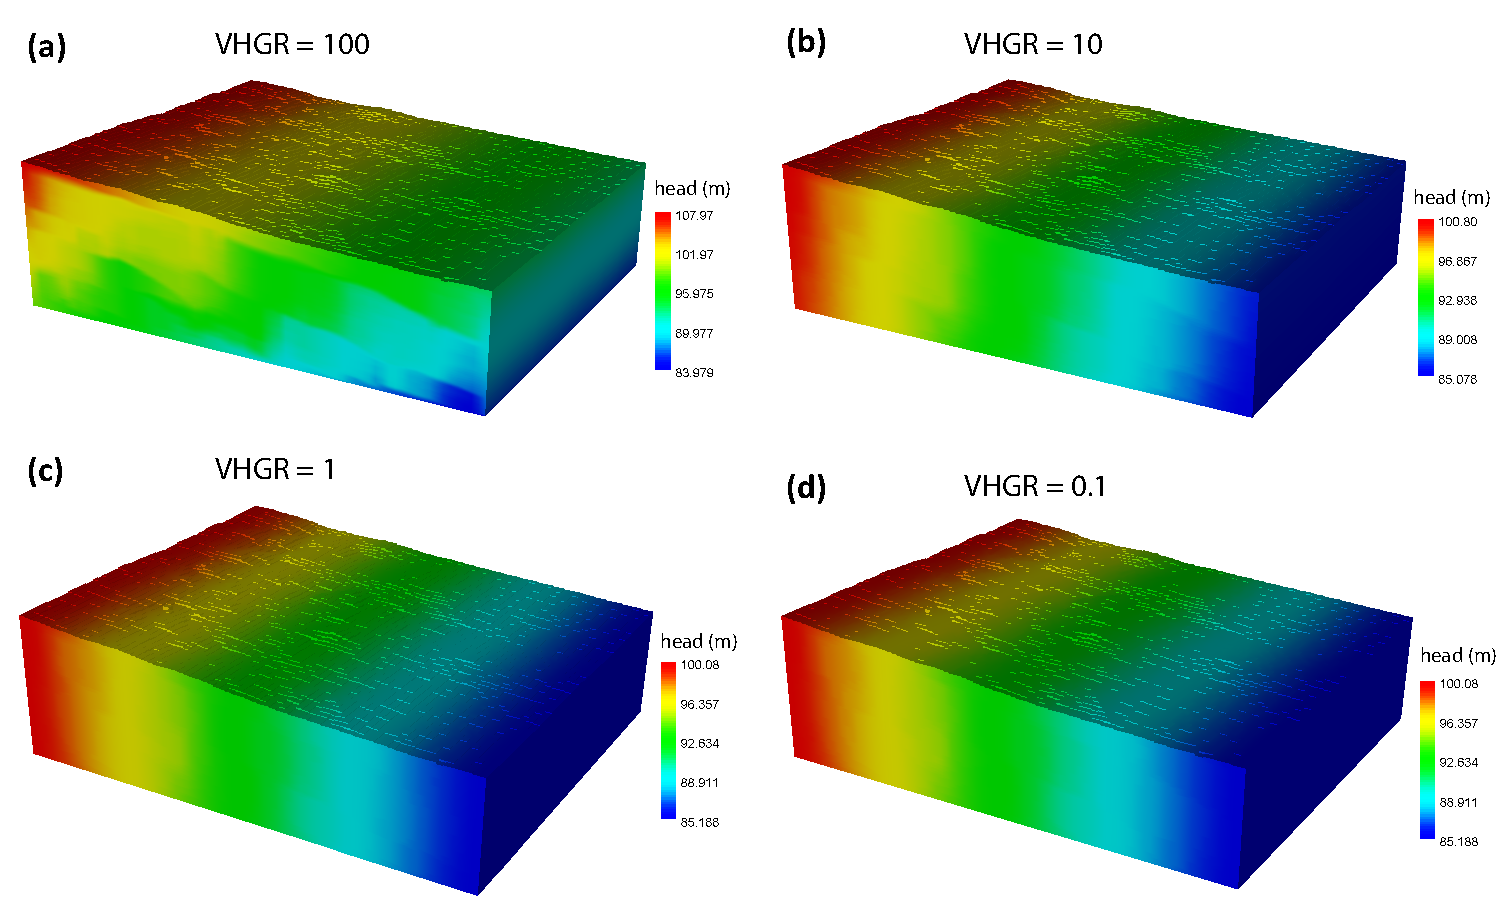
\includegraphics[width=\textwidth]{ch4_appendix_figs/heads.pdf}
  \caption{(a-d) Simulated steady state groundwater head across the 4 VHGR scenarios tested in this study.}
  \label{ap_c_heads_vhgr}
\end{figure}



%--------------------------------------------------------%
\subsection{Particle trajectory coordinate rotation and travel time normalization via the characteristic travel time}
\label{s_ap_c_part_rot}

In order to ensure comparability across the range of VHGR scenarios of differing travel times and mean flow direction, we perform coordinate rotations and normalize travel times by a characteristic travel time to travel the average facies length, $t_c$. 

First, we compute the mean Lagrangian velocity across all trajectories, $\bar{v}$ and use the characteristic time to travel the average facies length, $t_c$, to normalize time across VHGR scenarios (SI Appendix Table S1). The mean velocity and facies length are calculated along the direction of mean flow. Since this direction varies across VHGR, by an angle $\Phi$ relative to the horizontal direction, and the model outputs trajectories in a regular 3D Cartesian grid, we rotate the particle trajectory coordinates about the $x$ axis by $\Phi$ to recover the the transformed $y$ and $z$ components along the longitudinal and transverse vertical directions respectively ($y’$ and $z’$):

\begin{equation}
\begin{aligned}
\label{eq:rotation}
    y' = z \cdot sin(\Phi) + y \cdot cos(\Phi) \\
    z' = z \cdot cos(\Phi) - y \cdot sin(\Phi)
\end{aligned}
\end{equation}

Flow occurs along $zy$, thus the $x$ coordinates (transverse horizontal) remain unchanged. After transforming coordinates according to (\ref{eq:rotation}), we calculate longitudinal displacement along $y’$, transverse vertical displacement along $z’$, and transverse horizontal displacement along $x$.



\bgroup

\renewcommand{\arraystretch}{1.5}

\setlength{\tabcolsep}{20pt}

\begin{table}[H]

\caption{Mean velocity $\bar{v}$ along the longitudinal direction ($y'$), the angle of mean flow, relative to the horizontal direction in the un-rotated Cartesian coordinate system $\Phi$, the characteristic hydrofacies length $\lamdba_c$ along the longitudinal direction, and the characteristic time $t_c$ along the longitudinal direction ($t_c = l_c / \bar{v}$).} 
\centering


\begin{tabular}{lrrrr}
\label{ap_c_tc}

\textbf{VHGR} & $\bm{\Phi} (^{\circ})$ & $\bm{l_c \: \: (m)}$ & $\bm{\bar{v} \: \: (m/yr)}$ & $\bm{t_c \: \: (yr)}$  \\ 
\hline
   100 & 89.43 & 2.19  & 73.33 & 0.046 \\
   10  & 84.29 & 2.20  & 8.40  & 0.252 \\
   1   & 45.00 & 3.09  & 7.20  & 0.093 \\
   0.1 & 5.71  & 21.97 & 53.01 & 0.319 \\
\hline
\end{tabular}

\end{table}
\egroup




%--------------------------------------------------------%
\subsection{RW3D parameters}


% 01_mm_plots_tables.R in F:/ ... POst_QE_Research/DISSERTATION/01_mm
% search for gw_and_sw_c_summary table


\bgroup

\renewcommand{\arraystretch}{1.5}

\setlength{\tabcolsep}{20pt}

\begin{table}[H]

\caption{RW3D parameters for each VHGR scenario including the number of injected particles (particle count), the maximum simulation time (max time), and the number of snapshots saved (snapshot count). Note that the snapshot count = max time $\cdot$ 10 000, meaning that for each scenario, 100 snapshots were taken per year of simulation time.} 
\centering

\begin{tabular}{lrrr}
\label{ap_c_rw3d_params}

\textbf{VHGR} & \textbf{particle count} & \textbf{max time (yrs)} & \textbf{snapshot count}  \\ 
\hline
   100 & 10 000  & 100   & 10 000  \\
   10  & 10 000  & 500   & 50 000  \\
   1   & 10 000  & 1000 & 100 000 \\
   0.1 & 10 000  & 5000 & 500 000 \\
\hline
\end{tabular}

\end{table}
\egroup








%--------------------------------------------------------%
\subsection{Hydrofacies proportions over time}



\begin{figure}[H]
  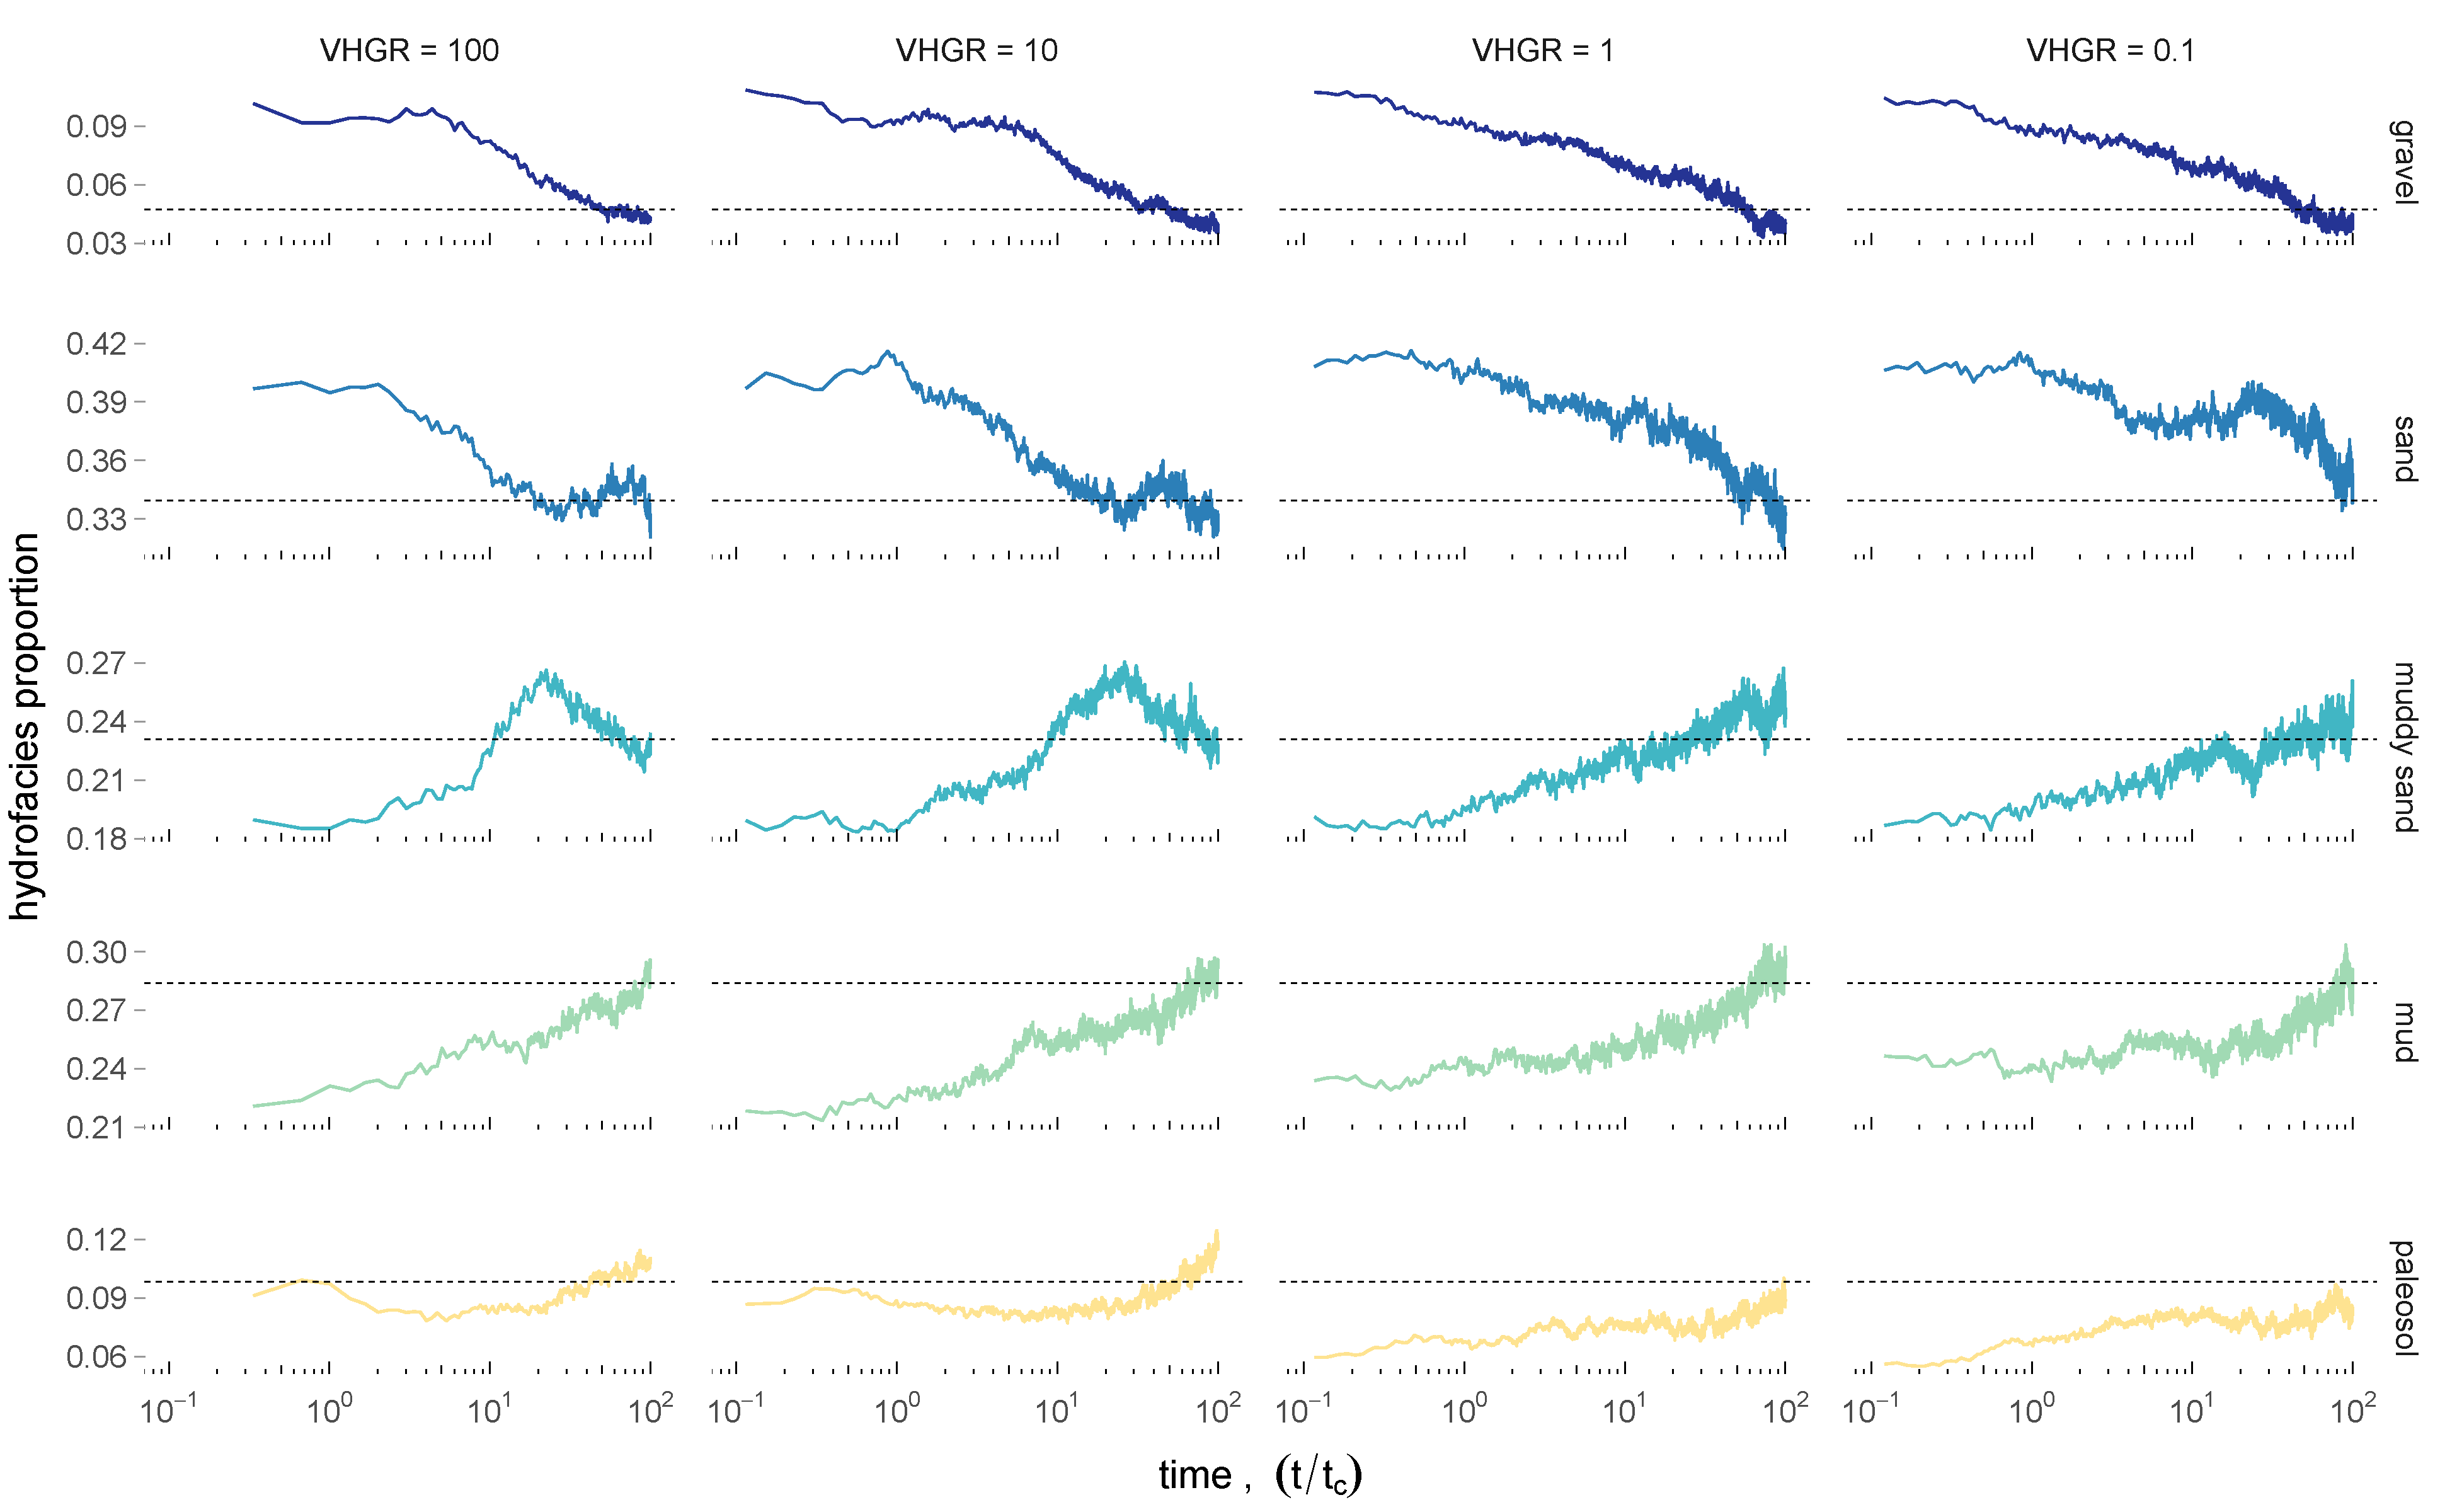
\includegraphics[width=\textwidth]{ch4_appendix_figs/phf_over_time_00_03_ai.pdf}
  \caption{Proportion of hydrofacies occupied by the particles as a function of time across the 4 VHGR scenarios indicate mixing: over about 32 characteristic times, proportions converge onto the hydrofacies proportions shown as black, dashed horizontal lines. Note the difference in y axis between the rows, each of which correspond to a distinct hydrofacies..}
  \label{ap_c_heads_vhgr}
\end{figure}



\clearpage



%--------------------------------------------------------%
% Acknowledgments
%--------------------------------------------------------%
\section{Acknowledgments}

We gratefully thank Drs. Yong Zhang, Marco Dentz, and Song Wei for their feedback and modeling advice. Support for this research was provided by the National Science Foundation (NSF) Climate Change, Water, and Society (CCWAS) Integrated Graduate Education and Research Traineeship (IGERT) program at the University of California, Davis (http://ccwas.ucdavis.edu, DGE-10693333), and by the U.S./China Clean Energy Research Center for Water-Energy Technologies (CERC-WET). %All data is accessible via Dryad at \textit{URL WITH DOI TO BE INPUT}, and procedures and models are accessible via Github at \textit{URL WITH DOI TO BE INPUT}.  




\clearpage
%\printbibliography[heading=bibliography]

% chapter 5
%\chapter{Real Title Here}
\chapter[Concluding Remarks.]{Concluding Remarks}

Writing near the turn of the 21st century, Dr. Norman Borlaug, a Nobel Laureate and key figure in the Green Revolution credited with pivotal advancements in plant genetics, noted that the continued success of the Green Revolution depended on fresh water availability, and called for a ``Blue Revolution'' to secure reliable water resources. Civilization's reliance on unsustainable groundwater pumping, especially in clastic sedimentary groundwater basins found in arid and semi-arid regions worldwide, limits the lifespan of these freshwater stores \citep{Scanlon2012, wada2010global, Gleeson2012}. For example, in California's Central Valley, aquifer lifespan has been estimated at 390 years or less depending on the exact location and depletion rate \citep{Scanlon2012}. Although aquifer depletion poses a long-term existential threat, a range of negative consequences (e.g., land subsidence, surface water depletion, destruction of groundwater-dependent ecosystems) will impact surface and groundwater systems long before aquifer stores run dangerously low, and these impacts will be exacerbated by surface water shortages in a warming climate \citep{Rhoades2018, Swain2018, Cook2015}, which has historically increased groundwater pumping to augment lost surface water supply \citep{Hanak2011, Medellin-azuara2016}. Thus, by addressing the short term consequences of aquifer depletion, the larger and slower-moving existential threat of aquifer depletion is also mitigated. 

This dissertation focuses on the development of models to address two understudied consequences of aquifer depletion: well failure and closed basin salinization. Chapter 2 demonstrates how data assimilation from monitoring well networks and open data from state agencies can be combined into a physical model of well failure that forecasts the impact of extended drought duration, groundwater management regimes, and wet winter recharge events in California's Central Valley. Chapter 4 advances a conceptual model of Anthropogenic Basin Closure and groundwater SALinization (ABCSAL), and first-order estimates of salinization in California's Tulare Basin. Chapter 3 uses 3D numerical flow and transport modeling in a complex hydrofacis model to show that transience in the mean flow direction caused by naturally-occurring (due to natural anisotropy in K) and induced hydraulic gradient transience (from pumping and recharge) can change the governing mass transfer processes in hyrdofacies, leading to differing degrees of non-Fickian transport. 


Chapter 2 demonstrates the vulnerability of domestic wells to both naturally-occurring hydrologic events (e.g., drought and wet winter recharge) and human-made water management decisions (e.g., sustainable and business as usual management regimes). Results indicate that extended drought durations (e.g., 5 to 8 years) can lead to a greater annual rate of well failure than observed during historic droughts (e.g., 2012-2016) as groundwater levels intersect an increasingly dense portion of the distribution of domestic well pump depths. Moreover, human water management decisons matter. Four times as many wells failed--even when controlling for hydrologic uncertainty--between a strict sustainability scenario in which groundwater levels were not allowed to fall after 2020, compared to a business as usual scenario that projected current groundwater level decline trends into 2040. Wet winter recharge events, and hence reduced pumping \citep{Hanak2019} and flood-based managed aquifer recharge \citep{Kocis2017} show potential to lessen the degree of domestic well failure. Looking forward, as Internet-of-things technologies mature and remote sensor networks are increasingly cost-effective and easy to maintain, the real-time monitoring of groundwater \citep{calderwood2020low} will permit data-driven models like the one presented in this study to automatically assimilate real-time groundwater level data and provide on-the-fly well failure risk estimates. Thus, it is conceivable that an early warning system for domestic well failure--not unlike existing early warning systems for drought \citep{pozzi2013toward, huang2004drought}--may be a future possibility enabled by sensor technology and cloud computing.

Similarly to Chapter 2, the topic of Chapter 3 remains understudied due to its relatively new emergence. Chapter 3 explores a mechanism by which groundwater pumping eliminates hydrologic exits for naturally-occurring salts in a basin (e.g., via baseflow and lateral subsurface outflow), after which those entrained salts accumulate in shallow aquifers due recycling from pumping and irrigation, before they are driven into deeper aquifer over century-long timescales. We call this process Anthropogenic Basin Closure and groundwater SALinization (ABCSAL). Importantly, results from a first-order mixing cell model indicate that shallow aquifers reach drinking water minimum thresholds for total dissolved solids (TDS) within decades, a result consistent with measurements of shallow aquifer TDS increase in the past century in the study site \citep{Hansen2018}. These results suggest that one mechanism to reverse or slow ongoing ABSCAL may include ``filling the basin up'' with significant recharge to restore baseflow and lateral subsurface outflow. Although the practical reality of such a management action may be cost-prohibitive or physically limited by available surface water in the Tulare Basin, it remains a viable solution in other basins worldwide experiencing ABCSAL. Moreover, a greater emphasis on subsurface water storage will require tightly monitoring and managing the ground and surface water interactions with distributed sensor networks, in order to prevent capillary rise and salinization from bare soil evaporation \citep{belitz1995alternative}. Without these mitigative management actions, ongoing and long-term ABCSAL may require inland desalinization of pumped groundwater.

Building on the work presented in Chapter 3, Chapter 4 uses 3D numerical groundwater flow and transport simulations in a detailed hydrofacies model with large variance in K \citep{weissmann1999multi} to better understand how hydraulic transience in the mean flow direction influences the degree of non-Fickian transport observed in hydrogeologic systems (e.g., nonpoint source salts discussed in Chapter 2). In California's Central Valley and other typical clastic sedimentary alluvial aquifer-aquitard systems worldwide, high vertical anisotropy in K naturally created by the inter-bedding of high and low K sediments, combined with pumping and recharge, can create flow systems that oscillate between predominately vertical and horizontal flow. Although other studies have noted that classical methods to upscale transport fail to represent tailing when the mean flow direction changes \citep{guo2019upscaling, guo2020adaptive}, the hydrogeologic underpinnings of this phenomenon remain poorly understood. Results indicate that relatively higher vertical to horizontal gradient ratio (VHGR) coincident with increasingly vertical mean flow direction can transition low-K facies from diffusion- to advection-dominant, and cause vertical groundwater flow to move directly through facies that typically act as aquitards at lower VHGR (e.g., paleosols, clays, and silts). In other words, when systems transition from diffusion- to advection-dominant, non-Fickian behavior (e.g., tailing, spatial variance, preferential flow) all decrease. These results imply a conceptual model of oscillating patterns in the degree of non-Fickian transport that correspond to seasonal patterns of pumping and recharge. Hence, non-Fickian transport models will better characterize flow systems under higher VHGR, depending on the gradients, characteristic facies length scales, and the Peclet number ($P_e$) of the distinct hydrofacies which describes the ratio of advection to diffusion time scales. These results also suggest a physical mechanism for arsenic leeching from low-K clays observed in the Central Valley during periods of land subsidence \citep{smith2018overpumping}, driven by advective flushing as strong vertical gradients ``force'' groundwater through clays. Lastly, the strong dependence of mass transfer on hydrogeologic features illustrated in this study suggests that future efforts to upscale regional-scale, transient nonpoint source transport may benefit by incorporating information on the time-dependent changes in VHGR, $P_e$, mean flow direction, and characteristic length scales along the direction of mean flow.

Securing sustainable groundwater resources in the 21st century and beyond will require the further development and refinement of hydrogeologic science, and numerical and data-driven models to assimilate that understanding and provide critical insights. Although this dissertation focuses on groundwater problems in California, the themes explored herein are extensible to other heavily pumped groundwater systems worldwide. Indeed, it is only through enhanced understand of aquifers that civilization may bring about a Blue Revolution in groundwater resources monitoring, modeling, and management.

\clearpage %This looks for chapter5_conclusion.tex
\printbibliography[heading=bibliography]


% note that the 'plainnat' style does not allow URL's in the bibtex entry
%
% some ideas here:
% http://bib2web.djvuzone.org/bibtex.html
%

% reset the page style
%\pagestyle{plain}


% To enable this it will need to be added to toc so it's not in a chapter
%\printbibliography[heading=bibliography]

% the appendix:
% there are several sections, that don't really fit into the main chapters
%
%\part*{\addcontentsline{toc}{part}{Appendices}Appendices}
  
%\appendix
%\renewcommand{\thepart}{\Alph{part}}
%\renewcommand{\thesection}{\Alph{section}}
%\renewcommand{\thesubsection}{\arabic{subsection}}
%\renewcommand\thefigure{\thesection.\arabic{figure}}
%\renewcommand\thetable{\thesection.\arabic{table}}
%\setcounter{figure}{0}    
%\setcounter{table}{0}    
%\setcounter{section}{0}



%\input{appendixCh1}
%\printbibliography[heading=bibliography]

%%\renewcommand\thefigure{\thesection.\arabic{figure}}    
\section{Tables of CVHM and C2VSim Generalized Flow Components and Model Variables}
%%%%%%%%%%%%
% TABLES %
%%%%%%%%%%%%

\input{ch3_tables/CVHM_landscape.tex}
\input{ch3_tables/CVHM_groundwater.tex}
\input{ch3_tables/C2VSim_landscape.tex}
\input{ch3_tables/C2VSim_groundwater.tex}
\newpage

\section{CVHM and C2VSim Water Budget Figures} \label{app:compare_figs}
%%%%%%%%%%%%
% FIG TEXT %
%%%%%%%%%%%%

%GW budget fig text
\newcommand{\GWBudgetText}{C2VSim and CVHM estimated cumulative annual change in groundwater storage, along with linear groundwater storage trends and annual change in storage volumes during 1962-2003 for }

%GW budget combined bar fig text
\newcommand{\GWCombinedTextOne}{Annual groundwater budget components from C2VSim and CVHM for }
\newcommand{\GWCombinedTextTwo}{ Flows into the groundwater system include landscape recharge, surface water gains, and net flows in from boundaries and adjacent subregions. Flows out include groundwater pumping, losses to surface water, and net flows out from boundaries and adjacent subregions}

%GW budget multi bar fig text
\newcommand{\GWMultiTextOne}{Comparison of similar annual groundwater budget components from C2VSim and CVHM for }
\newcommand{\GWMultiTextTwo}{ including similar flow components and total flows into (A) and out of (B) the groundwater system, along with statistical measures of the correspondence between similar flow components for each model (C), including normalized root mean square error (NRMSE) and correlation (Pearson's $r$).}

%Hyd prop box fig text
\newcommand{\HydPropOne}{Box plots of hydraulic properties of model layers in CVHM and C2VSim for }
\newcommand{\HydPropTwo}{ including horizontal and vertical hydraulic conductivity ($K$) and storage properties, which are represented by specific storage ($Ss$) for all layers in CVHM, and by specific yield for layer 1 and Ss in layers 3-4 in C2VSim*. The Corcoran Clay is represented by layers 4-5 and 2 in CVHM and C2VSim, respectively, and is only represented for some subregions, where it is present. C2VSim does not simulate horizontal K and storage properties for the Corcoran Clay. In general, CVHM layers 1-3, 4-5, 6-8, and 9-10 correspond with C2VSim layers 1, 2, 3, and 4, respectively.}

%LS budget combined bar fig text
\newcommand{\LSCombinedTextOne}{Annual landscape water budget components from C2VSim and CVHM for }
\newcommand{\LSCombinedTextTwo}{ Flows into the landscape include precipitation, surface water diversions, and groundwater pumping. Flows out include runoff and return flows, actual evapotranspiration ($ETa$), and deep percolation (i.e., recharge) to the groundwater system.}

%LS budget combined bar fig text
\newcommand{\LSMultiTextOne}{Comparison of similar annual landscape water budget components from C2VSim and CVHM for }
\newcommand{\LSMultiTextTwo}{ including similar flow components and total flows into (A) and out of (B) the landscape, along with statistical measures of the correspondence between similar flow components for each model (C), including normalized root mean square error (NRMSE), correlation (Pearson's $r$), and normalized mean bias (NMB).}

%%%%%%%%%%%%%%%%%%%%%%%%%
% ENTIRE CENTRAL VALLEY %
%%%%%%%%%%%%%%%%%%%%%%%%%

%GW budget fig
\subsection{Entire Central Valley}
\subsubsection{Groundwater Budget Components}
\begin{figure}[h]
\centerline{\includegraphics[width=130mm,keepaspectratio]{appendix_figs/GW_delta_stor_SR26.pdf}}
\caption{\GWBudgetText the entire Central Valley.}
\label{fig:delta_stor_SR26}
\end{figure}
\newpage

%GW budget combined bar fig
\begin{figure}[ht]
\centerline{\includegraphics[width=165mm,keepaspectratio]{appendix_figs/combined_bar_SR26.pdf}}
\caption{\GWCombinedTextOne the entire Central Valley.\GWCombinedTextTwo}
\label{fig:GW_budget_SR26}
\end{figure}
\newpage

%GW budget multi bar fig
\begin{landscape}
\begin{figure}[ht]
\centerline{\includegraphics[width=220mm,keepaspectratio]{appendix_figs/multi_bar_SR26.pdf}}
\caption{\GWMultiTextOne the entire Central Valley,\GWMultiTextTwo}
\label{fig:multi_GW_budget_SR26}
\end{figure}
\newpage

%Hyd prop box fig
\begin{figure}[ht]
\centerline{\includegraphics[width=180mm,keepaspectratio]{appendix_figs/hyd_prop_SR26.pdf}}
\caption{\HydPropOne the entire Central Valley,\HydPropTwo}
\label{fig:hyd_prop_SR26}
\end{figure}
\newpage
\end{landscape}

%LS budget combined bar fig
\subsubsection{Landscape Water Budget Components}
\begin{figure}[ht]
\centerline{\includegraphics[width=165mm,keepaspectratio]{appendix_figs/ls_combined_bar_SR26.pdf}}
\caption{\LSCombinedTextOne the entire Central Valley.\LSCombinedTextTwo}
\label{fig:LS_budget_SR26}
\end{figure}
\newpage

%LS budget multi bar fig
\begin{landscape}
\begin{figure}[ht]
\centerline{\includegraphics[width=220mm,keepaspectratio]{appendix_figs/ls_multi_bar_SR26.pdf}}
\caption{\LSMultiTextOne the entire Central Valley,\LSMultiTextTwo}
\label{fig:multi_LS_budget_SR26}
\end{figure}
\newpage
\end{landscape}

%%%%%%%%%%%%%%%%%%%%%
% SACRAMENTO REGION %
%%%%%%%%%%%%%%%%%%%%%
%GW budget fig
\subsection{Sacramento Valley Region}
\subsubsection{Groundwater Budget Components}
\begin{figure}[h]
\centerline{\includegraphics[width=130mm,keepaspectratio]{appendix_figs/GW_delta_stor_SR22.pdf}}
\caption{\GWBudgetText the Sacramento Valley Region.}
\label{fig:delta_stor_SR22}
\end{figure}
\newpage

%GW budget combined bar fig
\begin{figure}[ht]
\centerline{\includegraphics[width=165mm,keepaspectratio]{appendix_figs/combined_bar_SR22.pdf}}
\caption{\GWCombinedTextOne the Sacramento Valley Region.\GWCombinedTextTwo}
\label{fig:GW_budget_SR22}
\end{figure}
\newpage

%GW budget multi bar fig
\begin{landscape}
\begin{figure}[ht]
\centerline{\includegraphics[width=220mm,keepaspectratio]{appendix_figs/multi_bar_SR22.pdf}}
\caption{\GWMultiTextOne the Sacramento Valley Region,\GWMultiTextTwo}
\label{fig:multi_GW_budget_SR22}
\end{figure}
\newpage

%Hyd prop box fig
\begin{figure}[ht]
\centerline{\includegraphics[width=180mm,keepaspectratio]{appendix_figs/hyd_prop_SR22.pdf}}
\caption{\HydPropOne the Sacramento Valley Region,\HydPropTwo}
\label{fig:hyd_prop_SR22}
\end{figure}
\newpage
\end{landscape}

%LS budget combined bar fig
\subsubsection{Landscape Water Budget Components}
\begin{figure}[ht]
\centerline{\includegraphics[width=165mm,keepaspectratio]{appendix_figs/ls_combined_bar_SR22.pdf}}
\caption{\LSCombinedTextOne the Sacramento Valley Region.\LSCombinedTextTwo}
\label{fig:LS_budget_SR22}
\end{figure}
\newpage

%LS budget multi bar fig
\begin{landscape}
\begin{figure}[ht]
\centerline{\includegraphics[width=220mm,keepaspectratio]{appendix_figs/ls_multi_bar_SR22.pdf}}
\caption{\LSMultiTextOne the Sacramento Valley Region,\LSMultiTextTwo}
\label{fig:multi_LS_budget_SR22}
\end{figure}
\newpage
\end{landscape}

%%%%%%%%%%%%%%%%%%%%%%%%%%%%%%%%%%
% DELTA & E. SIDE STREAMS REGION %
%%%%%%%%%%%%%%%%%%%%%%%%%%%%%%%%%%
%GW budget fig
\subsection{Delta and East Side Streams}
\subsubsection{Groundwater Budget Components}
\begin{figure}[h]
\centerline{\includegraphics[width=130mm,keepaspectratio]{appendix_figs/GW_delta_stor_SR23.pdf}}
\caption{\GWBudgetText the Delta and East Side Streams.}
\label{fig:delta_stor_SR23}
\end{figure}
\newpage

%GW budget combined bar fig
\begin{figure}[ht]
\centerline{\includegraphics[width=165mm,keepaspectratio]{appendix_figs/combined_bar_SR23.pdf}}
\caption{\GWCombinedTextOne the Delta and East Side Streams.\GWCombinedTextTwo}
\label{fig:GW_budget_SR23}
\end{figure}
\newpage

%GW budget multi bar fig
\begin{landscape}
\begin{figure}[ht]
\centerline{\includegraphics[width=220mm,keepaspectratio]{appendix_figs/multi_bar_SR23.pdf}}
\caption{\GWMultiTextOne the Delta and East Side Streams,\GWMultiTextTwo}
\label{fig:multi_GW_budget_SR23}
\end{figure}
\newpage

%Hyd prop box fig
\begin{figure}[ht]
\centerline{\includegraphics[width=180mm,keepaspectratio]{appendix_figs/hyd_prop_SR23.pdf}}
\caption{\HydPropOne the Delta and East Side Streams,\HydPropTwo}
\label{fig:hyd_prop_SR23}
\end{figure}
\newpage
\end{landscape}

%LS budget combined bar fig
\subsubsection{Landscape Water Budget Components}
\begin{figure}[ht]
\centerline{\includegraphics[width=165mm,keepaspectratio]{appendix_figs/ls_combined_bar_SR23.pdf}}
\caption{\LSCombinedTextOne the Delta and East Side Streams.\LSCombinedTextTwo}
\label{fig:LS_budget_SR23}
\end{figure}
\newpage

%LS budget multi bar fig
\begin{landscape}
\begin{figure}[ht]
\centerline{\includegraphics[width=220mm,keepaspectratio]{appendix_figs/ls_multi_bar_SR23.pdf}}
\caption{\LSMultiTextOne the Delta and East Side Streams,\LSMultiTextTwo}
\label{fig:multi_LS_budget_SR23}
\end{figure}
\newpage
\end{landscape}

%%%%%%%%%%%%%%%%%%%%%%
% SAN JOAQUIN REGION %
%%%%%%%%%%%%%%%%%%%%%%
%GW budget fig
\subsection{San Joaquin Valley Region}
\subsubsection{Groundwater Budget Components}
\begin{figure}[h]
\centerline{\includegraphics[width=130mm,keepaspectratio]{appendix_figs/GW_delta_stor_SR24.pdf}}
\caption{\GWBudgetText the San Joaquin Valley Region.}
\label{fig:delta_stor_SR24}
\end{figure}
\newpage

%GW budget combined bar fig
\begin{figure}[ht]
\centerline{\includegraphics[width=165mm,keepaspectratio]{appendix_figs/combined_bar_SR24.pdf}}
\caption{\GWCombinedTextOne the San Joaquin Valley Region.\GWCombinedTextTwo}
\label{fig:GW_budget_SR24}
\end{figure}
\newpage

%GW budget multi bar fig
\begin{landscape}
\begin{figure}[ht]
\centerline{\includegraphics[width=220mm,keepaspectratio]{appendix_figs/multi_bar_SR24.pdf}}
\caption{\GWMultiTextOne the San Joaquin Valley Region,\GWMultiTextTwo}
\label{fig:multi_GW_budget_SR24}
\end{figure}
\newpage

%Hyd prop box fig
\begin{figure}[ht]
\centerline{\includegraphics[width=180mm,keepaspectratio]{appendix_figs/hyd_prop_SR24.pdf}}
\caption{\HydPropOne the San Joaquin Valley Region,\HydPropTwo}
\label{fig:hyd_prop_SR24}
\end{figure}
\newpage
\end{landscape}

%LS budget combined bar fig
\subsubsection{Landscape Water Budget Components}
\begin{figure}[ht]
\centerline{\includegraphics[width=165mm,keepaspectratio]{appendix_figs/ls_combined_bar_SR24.pdf}}
\caption{\LSCombinedTextOne the San Joaquin Valley Region.\LSCombinedTextTwo}
\label{fig:LS_budget_SR24}
\end{figure}
\newpage

%LS budget multi bar fig
\begin{landscape}
\begin{figure}[ht]
\centerline{\includegraphics[width=220mm,keepaspectratio]{appendix_figs/ls_multi_bar_SR24.pdf}}
\caption{\LSMultiTextOne the San Joaquin Valley Region,\LSMultiTextTwo}
\label{fig:multi_LS_budget_SR24}
\end{figure}
\newpage
\end{landscape}

%%%%%%%%%%%%%%%%%
% TULARE REGION %
%%%%%%%%%%%%%%%%%
%GW budget fig
\subsection{Tulare Lake Region}
\subsubsection{Groundwater Budget Components}
\begin{figure}[h]
\centerline{\includegraphics[width=130mm,keepaspectratio]{appendix_figs/GW_delta_stor_SR25.pdf}}
\caption{\GWBudgetText the Tulare Lake Region.}
\label{fig:delta_stor_SR25}
\end{figure}
\newpage

%GW budget combined bar fig
\begin{figure}[ht]
\centerline{\includegraphics[width=165mm,keepaspectratio]{appendix_figs/combined_bar_SR25.pdf}}
\caption{\GWCombinedTextOne the Tulare Lake Region.\GWCombinedTextTwo}
\label{fig:GW_budget_SR25}
\end{figure}
\newpage

%GW budget multi bar fig
\begin{landscape}
\begin{figure}[ht]
\centerline{\includegraphics[width=220mm,keepaspectratio]{appendix_figs/multi_bar_SR25.pdf}}
\caption{\GWMultiTextOne the Tulare Lake Region,\GWMultiTextTwo}
\label{fig:multi_GW_budget_SR25}
\end{figure}
\newpage

%Hyd prop box fig
\begin{figure}[ht]
\centerline{\includegraphics[width=180mm,keepaspectratio]{appendix_figs/hyd_prop_SR25.pdf}}
\caption{\HydPropOne the Tulare Lake Region,\HydPropTwo}
\label{fig:hyd_prop_SR25}
\end{figure}
\newpage
\end{landscape}

%LS budget combined bar fig
\subsubsection{Landscape Water Budget Components}
\begin{figure}[ht]
\centerline{\includegraphics[width=165mm,keepaspectratio]{appendix_figs/ls_combined_bar_SR25.pdf}}
\caption{\LSCombinedTextOne the Tulare Lake Region.\LSCombinedTextTwo}
\label{fig:LS_budget_SR25}
\end{figure}
\newpage

%LS budget multi bar fig
\begin{landscape}
\begin{figure}[ht]
\centerline{\includegraphics[width=220mm,keepaspectratio]{appendix_figs/ls_multi_bar_SR25.pdf}}
\caption{\LSMultiTextOne the Tulare Lake Region,\LSMultiTextTwo}
\label{fig:multi_LS_budget_SR25}
\end{figure}
\newpage
\end{landscape}

%%%%%%%%%%%%%%%
% SUBREGION 1 %
%%%%%%%%%%%%%%%

%GW budget fig
\subsection{Subregion 1}
\subsubsection{Groundwater Budget Components}
\begin{figure}[h]
\centerline{\includegraphics[width=130mm,keepaspectratio]{appendix_figs/GW_delta_stor_SR1.pdf}}
\caption{\GWBudgetText Subregion 1.}
\label{fig:delta_stor_SR1}
\end{figure}
\newpage

%GW budget combined bar fig
\begin{figure}[ht]
\centerline{\includegraphics[width=165mm,keepaspectratio]{appendix_figs/combined_bar_SR1.pdf}}
\caption{\GWCombinedTextOne Subregion 1.\GWCombinedTextTwo}
\label{fig:GW_budget_SR1}
\end{figure}
\newpage

%GW budget multi bar fig
\begin{landscape}
\begin{figure}[ht]
\centerline{\includegraphics[width=220mm,keepaspectratio]{appendix_figs/multi_bar_SR1.pdf}}
\caption{\GWMultiTextOne Subregion 1,\GWMultiTextTwo}
\label{fig:multi_GW_budget_SR1}
\end{figure}
\newpage

%Hyd prop box fig
\begin{figure}[ht]
\centerline{\includegraphics[width=180mm,keepaspectratio]{appendix_figs/hyd_prop_SR1.pdf}}
\caption{\HydPropOne Subregion 1,\HydPropTwo}
\label{fig:hyd_prop_SR1}
\end{figure}
\newpage
\end{landscape}

%LS budget combined bar fig
\subsubsection{Landscape Water Budget Components}
\begin{figure}[ht]
\centerline{\includegraphics[width=165mm,keepaspectratio]{appendix_figs/ls_combined_bar_SR1.pdf}}
\caption{\LSCombinedTextOne Subregion 1.\LSCombinedTextTwo}
\label{fig:LS_budget_SR1}
\end{figure}
\newpage

%LS budget multi bar fig
\begin{landscape}
\begin{figure}[ht]
\centerline{\includegraphics[width=220mm,keepaspectratio]{appendix_figs/ls_multi_bar_SR1.pdf}}
\caption{\LSMultiTextOne Subregion 1,\LSMultiTextTwo}
\label{fig:multi_LS_budget_SR1}
\end{figure}
\newpage
\end{landscape}

%%%%%%%%%%%%%%%
% SUBREGION 2 %
%%%%%%%%%%%%%%%
%GW budget fig
\subsection{Subregion 2}
\subsubsection{Groundwater Budget Components}
\begin{figure}[h]
\centerline{\includegraphics[width=130mm,keepaspectratio]{appendix_figs/GW_delta_stor_SR2.pdf}}
\caption{\GWBudgetText Subregion 2.}
\label{fig:delta_stor_SR2}
\end{figure}
\newpage

%GW budget combined bar fig
\begin{figure}[ht]
\centerline{\includegraphics[width=165mm,keepaspectratio]{appendix_figs/combined_bar_SR2.pdf}}
\caption{\GWCombinedTextOne Subregion 2.\GWCombinedTextTwo}
\label{fig:GW_budget_SR2}
\end{figure}
\newpage

%GW budget multi bar fig
\begin{landscape}
\begin{figure}[ht]
\centerline{\includegraphics[width=220mm,keepaspectratio]{appendix_figs/multi_bar_SR2.pdf}}
\caption{\GWMultiTextOne Subregion 2,\GWMultiTextTwo}
\label{fig:multi_GW_budget_SR2}
\end{figure}
\newpage

%Hyd prop box fig
\begin{figure}[ht]
\centerline{\includegraphics[width=180mm,keepaspectratio]{appendix_figs/hyd_prop_SR2.pdf}}
\caption{\HydPropOne Subregion 2,\HydPropTwo}
\label{fig:hyd_prop_SR2}
\end{figure}
\newpage
\end{landscape}

%LS budget combined bar fig
\subsubsection{Landscape Water Budget Components}
\begin{figure}[ht]
\centerline{\includegraphics[width=165mm,keepaspectratio]{appendix_figs/ls_combined_bar_SR2.pdf}}
\caption{\LSCombinedTextOne Subregion 2.\LSCombinedTextTwo}
\label{fig:LS_budget_SR2}
\end{figure}
\newpage

%LS budget multi bar fig
\begin{landscape}
\begin{figure}[ht]
\centerline{\includegraphics[width=220mm,keepaspectratio]{appendix_figs/ls_multi_bar_SR2.pdf}}
\caption{\LSMultiTextOne Subregion 2,\LSMultiTextTwo}
\label{fig:multi_LS_budget_SR2}
\end{figure}
\newpage
\end{landscape}

%%%%%%%%%%%%%%%
% SUBREGION 3 %
%%%%%%%%%%%%%%%
%GW budget fig
\subsection{Subregion 3}
\subsubsection{Groundwater Budget Components}
\begin{figure}[h]
\centerline{\includegraphics[width=130mm,keepaspectratio]{appendix_figs/GW_delta_stor_SR3.pdf}}
\caption{\GWBudgetText Subregion 3.}
\label{fig:delta_stor_SR3}
\end{figure}
\newpage

%GW budget combined bar fig
\begin{figure}[ht]
\centerline{\includegraphics[width=165mm,keepaspectratio]{appendix_figs/combined_bar_SR3.pdf}}
\caption{\GWCombinedTextOne Subregion 3.\GWCombinedTextTwo}
\label{fig:GW_budget_SR3}
\end{figure}
\newpage

%GW budget multi bar fig
\begin{landscape}
\begin{figure}[ht]
\centerline{\includegraphics[width=220mm,keepaspectratio]{appendix_figs/multi_bar_SR3.pdf}}
\caption{\GWMultiTextOne Subregion 3,\GWMultiTextTwo}
\label{fig:multi_GW_budget_SR3}
\end{figure}
\newpage

%Hyd prop box fig
\begin{figure}[ht]
\centerline{\includegraphics[width=180mm,keepaspectratio]{appendix_figs/hyd_prop_SR3.pdf}}
\caption{\HydPropOne Subregion 3,\HydPropTwo}
\label{fig:hyd_prop_SR3}
\end{figure}
\newpage
\end{landscape}

%LS budget combined bar fig
\subsubsection{Landscape Water Budget Components}
\begin{figure}[ht]
\centerline{\includegraphics[width=165mm,keepaspectratio]{appendix_figs/ls_combined_bar_SR3.pdf}}
\caption{\LSCombinedTextOne Subregion 3.\LSCombinedTextTwo}
\label{fig:LS_budget_SR3}
\end{figure}
\newpage

%LS budget multi bar fig
\begin{landscape}
\begin{figure}[ht]
\centerline{\includegraphics[width=220mm,keepaspectratio]{appendix_figs/ls_multi_bar_SR3.pdf}}
\caption{\LSMultiTextOne Subregion 3,\LSMultiTextTwo}
\label{fig:multi_LS_budget_SR3}
\end{figure}
\newpage
\end{landscape}

%%%%%%%%%%%%%%%
% SUBREGION 4 %
%%%%%%%%%%%%%%%
%GW budget fig
\subsection{Subregion 4}
\subsubsection{Groundwater Budget Components}
\begin{figure}[h]
\centerline{\includegraphics[width=130mm,keepaspectratio]{appendix_figs/GW_delta_stor_SR4.pdf}}
\caption{\GWBudgetText Subregion 4.}
\label{fig:delta_stor_SR4}
\end{figure}
\newpage

%GW budget combined bar fig
\begin{figure}[ht]
\centerline{\includegraphics[width=165mm,keepaspectratio]{appendix_figs/combined_bar_SR4.pdf}}
\caption{\GWCombinedTextOne Subregion 4.\GWCombinedTextTwo}
\label{fig:GW_budget_SR4}
\end{figure}
\newpage

%GW budget multi bar fig
\begin{landscape}
\begin{figure}[ht]
\centerline{\includegraphics[width=220mm,keepaspectratio]{appendix_figs/multi_bar_SR4.pdf}}
\caption{\GWMultiTextOne Subregion 4,\GWMultiTextTwo}
\label{fig:multi_GW_budget_SR4}
\end{figure}
\newpage

%Hyd prop box fig
\begin{figure}[ht]
\centerline{\includegraphics[width=180mm,keepaspectratio]{appendix_figs/hyd_prop_SR4.pdf}}
\caption{\HydPropOne Subregion 4,\HydPropTwo}
\label{fig:hyd_prop_SR4}
\end{figure}
\newpage
\end{landscape}

%LS budget combined bar fig
\subsubsection{Landscape Water Budget Components}
\begin{figure}[ht]
\centerline{\includegraphics[width=165mm,keepaspectratio]{appendix_figs/ls_combined_bar_SR4.pdf}}
\caption{\LSCombinedTextOne Subregion 4.\LSCombinedTextTwo}
\label{fig:LS_budget_SR4}
\end{figure}
\newpage

%LS budget multi bar fig
\begin{landscape}
\begin{figure}[ht]
\centerline{\includegraphics[width=220mm,keepaspectratio]{appendix_figs/ls_multi_bar_SR4.pdf}}
\caption{\LSMultiTextOne Subregion 4,\LSMultiTextTwo}
\label{fig:multi_LS_budget_SR4}
\end{figure}
\newpage
\end{landscape}

%%%%%%%%%%%%%%%
% SUBREGION 5 %
%%%%%%%%%%%%%%%
%GW budget fig
\subsection{Subregion 5}
\subsubsection{Groundwater Budget Components}
\begin{figure}[h]
\centerline{\includegraphics[width=130mm,keepaspectratio]{appendix_figs/GW_delta_stor_SR5.pdf}}
\caption{\GWBudgetText Subregion 5.}
\label{fig:delta_stor_SR5}
\end{figure}
\newpage

%GW budget combined bar fig
\begin{figure}[ht]
\centerline{\includegraphics[width=165mm,keepaspectratio]{appendix_figs/combined_bar_SR5.pdf}}
\caption{\GWCombinedTextOne Subregion 5.\GWCombinedTextTwo}
\label{fig:GW_budget_SR5}
\end{figure}
\newpage

%GW budget multi bar fig
\begin{landscape}
\begin{figure}[ht]
\centerline{\includegraphics[width=220mm,keepaspectratio]{appendix_figs/multi_bar_SR5.pdf}}
\caption{\GWMultiTextOne Subregion 5,\GWMultiTextTwo}
\label{fig:multi_GW_budget_SR5}
\end{figure}
\newpage

%Hyd prop box fig
\begin{figure}[ht]
\centerline{\includegraphics[width=180mm,keepaspectratio]{appendix_figs/hyd_prop_SR5.pdf}}
\caption{\HydPropOne Subregion 5,\HydPropTwo}
\label{fig:hyd_prop_SR5}
\end{figure}
\newpage
\end{landscape}

%LS budget combined bar fig
\subsubsection{Landscape Water Budget Components}
\begin{figure}[ht]
\centerline{\includegraphics[width=165mm,keepaspectratio]{appendix_figs/ls_combined_bar_SR5.pdf}}
\caption{\LSCombinedTextOne Subregion 5.\LSCombinedTextTwo}
\label{fig:LS_budget_SR5}
\end{figure}
\newpage

%LS budget multi bar fig
\begin{landscape}
\begin{figure}[ht]
\centerline{\includegraphics[width=220mm,keepaspectratio]{appendix_figs/ls_multi_bar_SR5.pdf}}
\caption{\LSMultiTextOne Subregion 5,\LSMultiTextTwo}
\label{fig:multi_LS_budget_SR5}
\end{figure}
\newpage
\end{landscape}

%%%%%%%%%%%%%%%
% SUBREGION 6 %
%%%%%%%%%%%%%%%
%GW budget fig
\subsection{Subregion 6}
\subsubsection{Groundwater Budget Components}
\begin{figure}[h]
\centerline{\includegraphics[width=130mm,keepaspectratio]{appendix_figs/GW_delta_stor_SR6.pdf}}
\caption{\GWBudgetText Subregion 6.}
\label{fig:delta_stor_SR6}
\end{figure}
\newpage

%GW budget combined bar fig
\begin{figure}[ht]
\centerline{\includegraphics[width=165mm,keepaspectratio]{appendix_figs/combined_bar_SR6.pdf}}
\caption{\GWCombinedTextOne Subregion 6.\GWCombinedTextTwo}
\label{fig:GW_budget_SR6}
\end{figure}
\newpage

%GW budget multi bar fig
\begin{landscape}
\begin{figure}[ht]
\centerline{\includegraphics[width=220mm,keepaspectratio]{appendix_figs/multi_bar_SR6.pdf}}
\caption{\GWMultiTextOne Subregion 6,\GWMultiTextTwo}
\label{fig:multi_GW_budget_SR6}
\end{figure}
\newpage

%Hyd prop box fig
\begin{figure}[ht]
\centerline{\includegraphics[width=180mm,keepaspectratio]{appendix_figs/hyd_prop_SR6.pdf}}
\caption{\HydPropOne Subregion 6,\HydPropTwo}
\label{fig:hyd_prop_SR6}
\end{figure}
\newpage
\end{landscape}

%LS budget combined bar fig
\subsubsection{Landscape Water Budget Components}
\begin{figure}[ht]
\centerline{\includegraphics[width=165mm,keepaspectratio]{appendix_figs/ls_combined_bar_SR6.pdf}}
\caption{\LSCombinedTextOne Subregion 6.\LSCombinedTextTwo}
\label{fig:LS_budget_SR6}
\end{figure}
\newpage

%LS budget multi bar fig
\begin{landscape}
\begin{figure}[ht]
\centerline{\includegraphics[width=220mm,keepaspectratio]{appendix_figs/ls_multi_bar_SR6.pdf}}
\caption{\LSMultiTextOne Subregion 6,\LSMultiTextTwo}
\label{fig:multi_LS_budget_SR6}
\end{figure}
\newpage
\end{landscape}

%%%%%%%%%%%%%%%
% SUBREGION 7 %
%%%%%%%%%%%%%%%
%GW budget fig
\subsection{Subregion 7}
\subsubsection{Groundwater Budget Components}
\begin{figure}[h]
\centerline{\includegraphics[width=130mm,keepaspectratio]{appendix_figs/GW_delta_stor_SR7.pdf}}
\caption{\GWBudgetText Subregion 7.}
\label{fig:delta_stor_SR7}
\end{figure}
\newpage

%GW budget combined bar fig
\begin{figure}[ht]
\centerline{\includegraphics[width=165mm,keepaspectratio]{appendix_figs/combined_bar_SR7.pdf}}
\caption{\GWCombinedTextOne Subregion 7.\GWCombinedTextTwo}
\label{fig:GW_budget_SR7}
\end{figure}
\newpage

%GW budget multi bar fig
\begin{landscape}
\begin{figure}[ht]
\centerline{\includegraphics[width=220mm,keepaspectratio]{appendix_figs/multi_bar_SR7.pdf}}
\caption{\GWMultiTextOne Subregion 7,\GWMultiTextTwo}
\label{fig:multi_GW_budget_SR7}
\end{figure}
\newpage

%Hyd prop box fig
\begin{figure}[ht]
\centerline{\includegraphics[width=180mm,keepaspectratio]{appendix_figs/hyd_prop_SR7.pdf}}
\caption{\HydPropOne Subregion 7,\HydPropTwo}
\label{fig:hyd_prop_SR7}
\end{figure}
\newpage
\end{landscape}

%LS budget combined bar fig
\subsubsection{Landscape Water Budget Components}
\begin{figure}[ht]
\centerline{\includegraphics[width=165mm,keepaspectratio]{appendix_figs/ls_combined_bar_SR7.pdf}}
\caption{\LSCombinedTextOne Subregion 7.\LSCombinedTextTwo}
\label{fig:LS_budget_SR7}
\end{figure}
\newpage

%LS budget multi bar fig
\begin{landscape}
\begin{figure}[ht]
\centerline{\includegraphics[width=220mm,keepaspectratio]{appendix_figs/ls_multi_bar_SR7.pdf}}
\caption{\LSMultiTextOne Subregion 7,\LSMultiTextTwo}
\label{fig:multi_LS_budget_SR7}
\end{figure}
\newpage
\end{landscape}

%%%%%%%%%%%%%%%
% SUBREGION 8 %
%%%%%%%%%%%%%%%
%GW budget fig
\subsection{Subregion 8}
\subsubsection{Groundwater Budget Components}
\begin{figure}[h]
\centerline{\includegraphics[width=130mm,keepaspectratio]{appendix_figs/GW_delta_stor_SR8.pdf}}
\caption{\GWBudgetText Subregion 8.}
\label{fig:delta_stor_SR8}
\end{figure}
\newpage

%GW budget combined bar fig
\begin{figure}[ht]
\centerline{\includegraphics[width=165mm,keepaspectratio]{appendix_figs/combined_bar_SR8.pdf}}
\caption{\GWCombinedTextOne Subregion 8.\GWCombinedTextTwo}
\label{fig:GW_budget_SR8}
\end{figure}
\newpage

%GW budget multi bar fig
\begin{landscape}
\begin{figure}[ht]
\centerline{\includegraphics[width=220mm,keepaspectratio]{appendix_figs/multi_bar_SR8.pdf}}
\caption{\GWMultiTextOne Subregion 8,\GWMultiTextTwo}
\label{fig:multi_GW_budget_SR8}
\end{figure}
\newpage

%Hyd prop box fig
\begin{figure}[ht]
\centerline{\includegraphics[width=180mm,keepaspectratio]{appendix_figs/hyd_prop_SR8.pdf}}
\caption{\HydPropOne Subregion 8,\HydPropTwo}
\label{fig:hyd_prop_SR8}
\end{figure}
\newpage
\end{landscape}

%LS budget combined bar fig
\subsubsection{Landscape Water Budget Components}
\begin{figure}[ht]
\centerline{\includegraphics[width=165mm,keepaspectratio]{appendix_figs/ls_combined_bar_SR8.pdf}}
\caption{\LSCombinedTextOne Subregion 8.\LSCombinedTextTwo}
\label{fig:LS_budget_SR8}
\end{figure}
\newpage

%LS budget multi bar fig
\begin{landscape}
\begin{figure}[ht]
\centerline{\includegraphics[width=220mm,keepaspectratio]{appendix_figs/ls_multi_bar_SR8.pdf}}
\caption{\LSMultiTextOne Subregion 8,\LSMultiTextTwo}
\label{fig:multi_LS_budget_SR8}
\end{figure}
\newpage
\end{landscape}

%%%%%%%%%%%%%%%
% SUBREGION 9 %
%%%%%%%%%%%%%%%
%GW budget fig
\subsection{Subregion 9}
\subsubsection{Groundwater Budget Components}
\begin{figure}[h]
\centerline{\includegraphics[width=130mm,keepaspectratio]{appendix_figs/GW_delta_stor_SR9.pdf}}
\caption{\GWBudgetText Subregion 9.}
\label{fig:delta_stor_SR9}
\end{figure}
\newpage

%GW budget combined bar fig
\begin{figure}[ht]
\centerline{\includegraphics[width=165mm,keepaspectratio]{appendix_figs/combined_bar_SR9.pdf}}
\caption{\GWCombinedTextOne Subregion 9.\GWCombinedTextTwo}
\label{fig:GW_budget_SR9}
\end{figure}
\newpage

%GW budget multi bar fig
\begin{landscape}
\begin{figure}[ht]
\centerline{\includegraphics[width=220mm,keepaspectratio]{appendix_figs/multi_bar_SR9.pdf}}
\caption{\GWMultiTextOne Subregion 9,\GWMultiTextTwo}
\label{fig:multi_GW_budget_SR9}
\end{figure}
\newpage

%Hyd prop box fig
\begin{figure}[ht]
\centerline{\includegraphics[width=180mm,keepaspectratio]{appendix_figs/hyd_prop_SR9.pdf}}
\caption{\HydPropOne Subregion 9,\HydPropTwo}
\label{fig:hyd_prop_SR9}
\end{figure}
\newpage
\end{landscape}

%LS budget combined bar fig
\subsubsection{Landscape Water Budget Components}
\begin{figure}[ht]
\centerline{\includegraphics[width=165mm,keepaspectratio]{appendix_figs/ls_combined_bar_SR9.pdf}}
\caption{\LSCombinedTextOne Subregion 9.\LSCombinedTextTwo}
\label{fig:LS_budget_SR9}
\end{figure}
\newpage

%LS budget multi bar fig
\begin{landscape}
\begin{figure}[ht]
\centerline{\includegraphics[width=220mm,keepaspectratio]{appendix_figs/ls_multi_bar_SR9.pdf}}
\caption{\LSMultiTextOne Subregion 9,\LSMultiTextTwo}
\label{fig:multi_LS_budget_SR9}
\end{figure}
\newpage
\end{landscape}

%%%%%%%%%%%%%%%
% SUBREGION 10 %
%%%%%%%%%%%%%%%
%GW budget fig
\subsection{Subregion 10}
\subsubsection{Groundwater Budget Components}
\begin{figure}[h]
\centerline{\includegraphics[width=130mm,keepaspectratio]{appendix_figs/GW_delta_stor_SR10.pdf}}
\caption{\GWBudgetText Subregion 10.}
\label{fig:delta_stor_SR10}
\end{figure}
\newpage

%GW budget combined bar fig
\begin{figure}[ht]
\centerline{\includegraphics[width=165mm,keepaspectratio]{appendix_figs/combined_bar_SR10.pdf}}
\caption{\GWCombinedTextOne Subregion 10.\GWCombinedTextTwo}
\label{fig:GW_budget_SR10}
\end{figure}
\newpage

%GW budget multi bar fig
\begin{landscape}
\begin{figure}[ht]
\centerline{\includegraphics[width=220mm,keepaspectratio]{appendix_figs/multi_bar_SR10.pdf}}
\caption{\GWMultiTextOne Subregion 10,\GWMultiTextTwo}
\label{fig:multi_GW_budget_SR10}
\end{figure}
\newpage

%Hyd prop box fig
\begin{figure}[ht]
\centerline{\includegraphics[width=180mm,keepaspectratio]{appendix_figs/hyd_prop_SR10.pdf}}
\caption{\HydPropOne Subregion 10,\HydPropTwo}
\label{fig:hyd_prop_SR10}
\end{figure}
\newpage
\end{landscape}

%LS budget combined bar fig
\subsubsection{Landscape Water Budget Components}
\begin{figure}[ht]
\centerline{\includegraphics[width=165mm,keepaspectratio]{appendix_figs/ls_combined_bar_SR10.pdf}}
\caption{\LSCombinedTextOne Subregion 10.\LSCombinedTextTwo}
\label{fig:LS_budget_SR10}
\end{figure}
\newpage

%LS budget multi bar fig
\begin{landscape}
\begin{figure}[ht]
\centerline{\includegraphics[width=220mm,keepaspectratio]{appendix_figs/ls_multi_bar_SR10.pdf}}
\caption{\LSMultiTextOne Subregion 10,\LSMultiTextTwo}
\label{fig:multi_LS_budget_SR10}
\end{figure}
\newpage
\end{landscape}

%%%%%%%%%%%%%%%
% SUBREGION 11 %
%%%%%%%%%%%%%%%
%GW budget fig
\subsection{Subregion 11}
\subsubsection{Groundwater Budget Components}
\begin{figure}[h]
\centerline{\includegraphics[width=130mm,keepaspectratio]{appendix_figs/GW_delta_stor_SR11.pdf}}
\caption{\GWBudgetText Subregion 11.}
\label{fig:delta_stor_SR11}
\end{figure}
\newpage

%GW budget combined bar fig
\begin{figure}[ht]
\centerline{\includegraphics[width=165mm,keepaspectratio]{appendix_figs/combined_bar_SR11.pdf}}
\caption{\GWCombinedTextOne Subregion 11.\GWCombinedTextTwo}
\label{fig:GW_budget_SR11}
\end{figure}
\newpage

%GW budget multi bar fig
\begin{landscape}
\begin{figure}[ht]
\centerline{\includegraphics[width=220mm,keepaspectratio]{appendix_figs/multi_bar_SR11.pdf}}
\caption{\GWMultiTextOne Subregion 11,\GWMultiTextTwo}
\label{fig:multi_GW_budget_SR11}
\end{figure}
\newpage

%Hyd prop box fig
\begin{figure}[ht]
\centerline{\includegraphics[width=180mm,keepaspectratio]{appendix_figs/hyd_prop_SR11.pdf}}
\caption{\HydPropOne Subregion 11,\HydPropTwo}
\label{fig:hyd_prop_SR11}
\end{figure}
\newpage
\end{landscape}

%LS budget combined bar fig
\subsubsection{Landscape Water Budget Components}
\begin{figure}[ht]
\centerline{\includegraphics[width=165mm,keepaspectratio]{appendix_figs/ls_combined_bar_SR11.pdf}}
\caption{\LSCombinedTextOne Subregion 11.\LSCombinedTextTwo}
\label{fig:LS_budget_SR11}
\end{figure}
\newpage

%LS budget multi bar fig
\begin{landscape}
\begin{figure}[ht]
\centerline{\includegraphics[width=220mm,keepaspectratio]{appendix_figs/ls_multi_bar_SR11.pdf}}
\caption{\LSMultiTextOne Subregion 11,\LSMultiTextTwo}
\label{fig:multi_LS_budget_SR11}
\end{figure}
\newpage
\end{landscape}

%%%%%%%%%%%%%%%
% SUBREGION 12 %
%%%%%%%%%%%%%%%
%GW budget fig
\subsection{Subregion 12}
\subsubsection{Groundwater Budget Components}
\begin{figure}[h]
\centerline{\includegraphics[width=130mm,keepaspectratio]{appendix_figs/GW_delta_stor_SR12.pdf}}
\caption{\GWBudgetText Subregion 12.}
\label{fig:delta_stor_SR12}
\end{figure}
\newpage

%GW budget combined bar fig
\begin{figure}[ht]
\centerline{\includegraphics[width=165mm,keepaspectratio]{appendix_figs/combined_bar_SR12.pdf}}
\caption{\GWCombinedTextOne Subregion 12.\GWCombinedTextTwo}
\label{fig:GW_budget_SR12}
\end{figure}
\newpage

%GW budget multi bar fig
\begin{landscape}
\begin{figure}[ht]
\centerline{\includegraphics[width=220mm,keepaspectratio]{appendix_figs/multi_bar_SR12.pdf}}
\caption{\GWMultiTextOne Subregion 12,\GWMultiTextTwo}
\label{fig:multi_GW_budget_SR12}
\end{figure}
\newpage

%Hyd prop box fig
\begin{figure}[ht]
\centerline{\includegraphics[width=180mm,keepaspectratio]{appendix_figs/hyd_prop_SR12.pdf}}
\caption{\HydPropOne Subregion 12,\HydPropTwo}
\label{fig:hyd_prop_SR12}
\end{figure}
\newpage
\end{landscape}

%LS budget combined bar fig
\subsubsection{Landscape Water Budget Components}
\begin{figure}[ht]
\centerline{\includegraphics[width=165mm,keepaspectratio]{appendix_figs/ls_combined_bar_SR12.pdf}}
\caption{\LSCombinedTextOne Subregion 12.\LSCombinedTextTwo}
\label{fig:LS_budget_SR12}
\end{figure}
\newpage

%LS budget multi bar fig
\begin{landscape}
\begin{figure}[ht]
\centerline{\includegraphics[width=220mm,keepaspectratio]{appendix_figs/ls_multi_bar_SR12.pdf}}
\caption{\LSMultiTextOne Subregion 12,\LSMultiTextTwo}
\label{fig:multi_LS_budget_SR12}
\end{figure}
\newpage
\end{landscape}

%%%%%%%%%%%%%%%
% SUBREGION 13 %
%%%%%%%%%%%%%%%
%GW budget fig
\subsection{Subregion 13}
\subsubsection{Groundwater Budget Components}
\begin{figure}[h]
\centerline{\includegraphics[width=130mm,keepaspectratio]{appendix_figs/GW_delta_stor_SR13.pdf}}
\caption{\GWBudgetText Subregion 13.}
\label{fig:delta_stor_SR13}
\end{figure}
\newpage

%GW budget combined bar fig
\begin{figure}[ht]
\centerline{\includegraphics[width=165mm,keepaspectratio]{appendix_figs/combined_bar_SR13.pdf}}
\caption{\GWCombinedTextOne Subregion 13.\GWCombinedTextTwo}
\label{fig:GW_budget_SR13}
\end{figure}
\newpage

%GW budget multi bar fig
\begin{landscape}
\begin{figure}[ht]
\centerline{\includegraphics[width=220mm,keepaspectratio]{appendix_figs/multi_bar_SR13.pdf}}
\caption{\GWMultiTextOne Subregion 13,\GWMultiTextTwo}
\label{fig:multi_GW_budget_SR13}
\end{figure}
\newpage

%Hyd prop box fig
\begin{figure}[ht]
\centerline{\includegraphics[width=180mm,keepaspectratio]{appendix_figs/hyd_prop_SR13.pdf}}
\caption{\HydPropOne Subregion 13,\HydPropTwo}
\label{fig:hyd_prop_SR13}
\end{figure}
\newpage
\end{landscape}

%LS budget combined bar fig
\subsubsection{Landscape Water Budget Components}
\begin{figure}[ht]
\centerline{\includegraphics[width=165mm,keepaspectratio]{appendix_figs/ls_combined_bar_SR13.pdf}}
\caption{\LSCombinedTextOne Subregion 13.\LSCombinedTextTwo}
\label{fig:LS_budget_SR13}
\end{figure}
\newpage

%LS budget multi bar fig
\begin{landscape}
\begin{figure}[ht]
\centerline{\includegraphics[width=220mm,keepaspectratio]{appendix_figs/ls_multi_bar_SR13.pdf}}
\caption{\LSMultiTextOne Subregion 13,\LSMultiTextTwo}
\label{fig:multi_LS_budget_SR13}
\end{figure}
\newpage
\end{landscape}

%%%%%%%%%%%%%%%
% SUBREGION 14 %
%%%%%%%%%%%%%%%
%GW budget fig
\subsection{Subregion 14}
\subsubsection{Groundwater Budget Components}
\begin{figure}[h]
\centerline{\includegraphics[width=130mm,keepaspectratio]{appendix_figs/GW_delta_stor_SR14.pdf}}
\caption{\GWBudgetText Subregion 14.}
\label{fig:delta_stor_SR14}
\end{figure}
\newpage

%GW budget combined bar fig
\begin{figure}[ht]
\centerline{\includegraphics[width=165mm,keepaspectratio]{appendix_figs/combined_bar_SR14.pdf}}
\caption{\GWCombinedTextOne Subregion 14.\GWCombinedTextTwo}
\label{fig:GW_budget_SR14}
\end{figure}
\newpage

%GW budget multi bar fig
\begin{landscape}
\begin{figure}[ht]
\centerline{\includegraphics[width=220mm,keepaspectratio]{appendix_figs/multi_bar_SR14.pdf}}
\caption{\GWMultiTextOne Subregion 14,\GWMultiTextTwo}
\label{fig:multi_GW_budget_SR14}
\end{figure}
\newpage

%Hyd prop box fig
\begin{figure}[ht]
\centerline{\includegraphics[width=180mm,keepaspectratio]{appendix_figs/hyd_prop_SR14.pdf}}
\caption{\HydPropOne Subregion 14,\HydPropTwo}
\label{fig:hyd_prop_SR14}
\end{figure}
\newpage
\end{landscape}

%LS budget combined bar fig
\subsubsection{Landscape Water Budget Components}
\begin{figure}[ht]
\centerline{\includegraphics[width=165mm,keepaspectratio]{appendix_figs/ls_combined_bar_SR14.pdf}}
\caption{\LSCombinedTextOne Subregion 14.\LSCombinedTextTwo}
\label{fig:LS_budget_SR14}
\end{figure}
\newpage

%LS budget multi bar fig
\begin{landscape}
\begin{figure}[ht]
\centerline{\includegraphics[width=220mm,keepaspectratio]{appendix_figs/ls_multi_bar_SR14.pdf}}
\caption{\LSMultiTextOne Subregion 14,\LSMultiTextTwo}
\label{fig:multi_LS_budget_SR14}
\end{figure}
\newpage
\end{landscape}

%%%%%%%%%%%%%%%
% SUBREGION 15 %
%%%%%%%%%%%%%%%
%GW budget fig
\subsection{Subregion 15}
\subsubsection{Groundwater Budget Components}
\begin{figure}[h]
\centerline{\includegraphics[width=130mm,keepaspectratio]{appendix_figs/GW_delta_stor_SR15.pdf}}
\caption{\GWBudgetText Subregion 15.}
\label{fig:delta_stor_SR15}
\end{figure}
\newpage

%GW budget combined bar fig
\begin{figure}[ht]
\centerline{\includegraphics[width=165mm,keepaspectratio]{appendix_figs/combined_bar_SR15.pdf}}
\caption{\GWCombinedTextOne Subregion 15.\GWCombinedTextTwo}
\label{fig:GW_budget_SR15}
\end{figure}
\newpage

%GW budget multi bar fig
\begin{landscape}
\begin{figure}[ht]
\centerline{\includegraphics[width=220mm,keepaspectratio]{appendix_figs/multi_bar_SR15.pdf}}
\caption{\GWMultiTextOne Subregion 15,\GWMultiTextTwo}
\label{fig:multi_GW_budget_SR15}
\end{figure}
\newpage

%Hyd prop box fig
\begin{figure}[ht]
\centerline{\includegraphics[width=180mm,keepaspectratio]{appendix_figs/hyd_prop_SR15.pdf}}
\caption{\HydPropOne Subregion 15,\HydPropTwo}
\label{fig:hyd_prop_SR15}
\end{figure}
\newpage
\end{landscape}

%LS budget combined bar fig
\subsubsection{Landscape Water Budget Components}
\begin{figure}[ht]
\centerline{\includegraphics[width=165mm,keepaspectratio]{appendix_figs/ls_combined_bar_SR15.pdf}}
\caption{\LSCombinedTextOne Subregion 15.\LSCombinedTextTwo}
\label{fig:LS_budget_SR15}
\end{figure}
\newpage

%LS budget multi bar fig
\begin{landscape}
\begin{figure}[ht]
\centerline{\includegraphics[width=220mm,keepaspectratio]{appendix_figs/ls_multi_bar_SR15.pdf}}
\caption{\LSMultiTextOne Subregion 15,\LSMultiTextTwo}
\label{fig:multi_LS_budget_SR15}
\end{figure}
\newpage
\end{landscape}

%%%%%%%%%%%%%%%
% SUBREGION 16 %
%%%%%%%%%%%%%%%
%GW budget fig
\subsection{Subregion 16}
\subsubsection{Groundwater Budget Components}
\begin{figure}[h]
\centerline{\includegraphics[width=130mm,keepaspectratio]{appendix_figs/GW_delta_stor_SR16.pdf}}
\caption{\GWBudgetText Subregion 16.}
\label{fig:delta_stor_SR16}
\end{figure}
\newpage

%GW budget combined bar fig
\begin{figure}[ht]
\centerline{\includegraphics[width=165mm,keepaspectratio]{appendix_figs/combined_bar_SR16.pdf}}
\caption{\GWCombinedTextOne Subregion 16.\GWCombinedTextTwo}
\label{fig:GW_budget_SR16}
\end{figure}
\newpage

%GW budget multi bar fig
\begin{landscape}
\begin{figure}[ht]
\centerline{\includegraphics[width=220mm,keepaspectratio]{appendix_figs/multi_bar_SR16.pdf}}
\caption{\GWMultiTextOne Subregion 16,\GWMultiTextTwo}
\label{fig:multi_GW_budget_SR16}
\end{figure}
\newpage

%Hyd prop box fig
\begin{figure}[ht]
\centerline{\includegraphics[width=180mm,keepaspectratio]{appendix_figs/hyd_prop_SR16.pdf}}
\caption{\HydPropOne Subregion 16,\HydPropTwo}
\label{fig:hyd_prop_SR16}
\end{figure}
\newpage
\end{landscape}

%LS budget combined bar fig
\subsubsection{Landscape Water Budget Components}
\begin{figure}[ht]
\centerline{\includegraphics[width=165mm,keepaspectratio]{appendix_figs/ls_combined_bar_SR16.pdf}}
\caption{\LSCombinedTextOne Subregion 16.\LSCombinedTextTwo}
\label{fig:LS_budget_SR16}
\end{figure}
\newpage

%LS budget multi bar fig
\begin{landscape}
\begin{figure}[ht]
\centerline{\includegraphics[width=220mm,keepaspectratio]{appendix_figs/ls_multi_bar_SR16.pdf}}
\caption{\LSMultiTextOne Subregion 16,\LSMultiTextTwo}
\label{fig:multi_LS_budget_SR16}
\end{figure}
\newpage
\end{landscape}

%%%%%%%%%%%%%%%
% SUBREGION 17 %
%%%%%%%%%%%%%%%
%GW budget fig
\subsection{Subregion 17}
\subsubsection{Groundwater Budget Components}
\begin{figure}[h]
\centerline{\includegraphics[width=130mm,keepaspectratio]{appendix_figs/GW_delta_stor_SR17.pdf}}
\caption{\GWBudgetText Subregion 17.}
\label{fig:delta_stor_SR17}
\end{figure}
\newpage

%GW budget combined bar fig
\begin{figure}[ht]
\centerline{\includegraphics[width=165mm,keepaspectratio]{appendix_figs/combined_bar_SR17.pdf}}
\caption{\GWCombinedTextOne Subregion 17.\GWCombinedTextTwo}
\label{fig:GW_budget_SR17}
\end{figure}
\newpage

%GW budget multi bar fig
\begin{landscape}
\begin{figure}[ht]
\centerline{\includegraphics[width=220mm,keepaspectratio]{appendix_figs/multi_bar_SR17.pdf}}
\caption{\GWMultiTextOne Subregion 17,\GWMultiTextTwo}
\label{fig:multi_GW_budget_SR17}
\end{figure}
\newpage

%Hyd prop box fig
\begin{figure}[ht]
\centerline{\includegraphics[width=180mm,keepaspectratio]{appendix_figs/hyd_prop_SR17.pdf}}
\caption{\HydPropOne Subregion 17,\HydPropTwo}
\label{fig:hyd_prop_SR17}
\end{figure}
\newpage
\end{landscape}

%LS budget combined bar fig
\subsubsection{Landscape Water Budget Components}
\begin{figure}[ht]
\centerline{\includegraphics[width=165mm,keepaspectratio]{appendix_figs/ls_combined_bar_SR17.pdf}}
\caption{\LSCombinedTextOne Subregion 17.\LSCombinedTextTwo}
\label{fig:LS_budget_SR17}
\end{figure}
\newpage

%LS budget multi bar fig
\begin{landscape}
\begin{figure}[ht]
\centerline{\includegraphics[width=220mm,keepaspectratio]{appendix_figs/ls_multi_bar_SR17.pdf}}
\caption{\LSMultiTextOne Subregion 17,\LSMultiTextTwo}
\label{fig:multi_LS_budget_SR17}
\end{figure}
\newpage
\end{landscape}

%%%%%%%%%%%%%%%
% SUBREGION 18 %
%%%%%%%%%%%%%%%
%GW budget fig
\subsection{Subregion 18}
\subsubsection{Groundwater Budget Components}
\begin{figure}[h]
\centerline{\includegraphics[width=130mm,keepaspectratio]{appendix_figs/GW_delta_stor_SR18.pdf}}
\caption{\GWBudgetText Subregion 18.}
\label{fig:delta_stor_SR18}
\end{figure}
\newpage

%GW budget combined bar fig
\begin{figure}[ht]
\centerline{\includegraphics[width=165mm,keepaspectratio]{appendix_figs/combined_bar_SR18.pdf}}
\caption{\GWCombinedTextOne Subregion 18.\GWCombinedTextTwo}
\label{fig:GW_budget_SR18}
\end{figure}
\newpage

%GW budget multi bar fig
\begin{landscape}
\begin{figure}[ht]
\centerline{\includegraphics[width=220mm,keepaspectratio]{appendix_figs/multi_bar_SR18.pdf}}
\caption{\GWMultiTextOne Subregion 18,\GWMultiTextTwo}
\label{fig:multi_GW_budget_SR18}
\end{figure}
\newpage

%Hyd prop box fig
\begin{figure}[ht]
\centerline{\includegraphics[width=180mm,keepaspectratio]{appendix_figs/hyd_prop_SR18.pdf}}
\caption{\HydPropOne Subregion 18,\HydPropTwo}
\label{fig:hyd_prop_SR18}
\end{figure}
\newpage
\end{landscape}

%LS budget combined bar fig
\subsubsection{Landscape Water Budget Components}
\begin{figure}[ht]
\centerline{\includegraphics[width=165mm,keepaspectratio]{appendix_figs/ls_combined_bar_SR18.pdf}}
\caption{\LSCombinedTextOne Subregion 18.\LSCombinedTextTwo}
\label{fig:LS_budget_SR18}
\end{figure}
\newpage

%LS budget multi bar fig
\begin{landscape}
\begin{figure}[ht]
\centerline{\includegraphics[width=220mm,keepaspectratio]{appendix_figs/ls_multi_bar_SR18.pdf}}
\caption{\LSMultiTextOne Subregion 18,\LSMultiTextTwo}
\label{fig:multi_LS_budget_SR18}
\end{figure}
\newpage
\end{landscape}

%%%%%%%%%%%%%%%
% SUBREGION 19 %
%%%%%%%%%%%%%%%
%GW budget fig
\subsection{Subregion 19}
\subsubsection{Groundwater Budget Components}
\begin{figure}[h]
\centerline{\includegraphics[width=130mm,keepaspectratio]{appendix_figs/GW_delta_stor_SR19.pdf}}
\caption{\GWBudgetText Subregion 19.}
\label{fig:delta_stor_SR19}
\end{figure}
\newpage

%GW budget combined bar fig
\begin{figure}[ht]
\centerline{\includegraphics[width=165mm,keepaspectratio]{appendix_figs/combined_bar_SR19.pdf}}
\caption{\GWCombinedTextOne Subregion 19.\GWCombinedTextTwo}
\label{fig:GW_budget_SR19}
\end{figure}
\newpage

%GW budget multi bar fig
\begin{landscape}
\begin{figure}[ht]
\centerline{\includegraphics[width=220mm,keepaspectratio]{appendix_figs/multi_bar_SR19.pdf}}
\caption{\GWMultiTextOne Subregion 19,\GWMultiTextTwo}
\label{fig:multi_GW_budget_SR19}
\end{figure}
\newpage

%Hyd prop box fig
\begin{figure}[ht]
\centerline{\includegraphics[width=180mm,keepaspectratio]{appendix_figs/hyd_prop_SR19.pdf}}
\caption{\HydPropOne Subregion 19,\HydPropTwo}
\label{fig:hyd_prop_SR19}
\end{figure}
\newpage
\end{landscape}

%LS budget combined bar fig
\subsubsection{Landscape Water Budget Components}
\begin{figure}[ht]
\centerline{\includegraphics[width=165mm,keepaspectratio]{appendix_figs/ls_combined_bar_SR19.pdf}}
\caption{\LSCombinedTextOne Subregion 19.\LSCombinedTextTwo}
\label{fig:LS_budget_SR19}
\end{figure}
\newpage

%LS budget multi bar fig
\begin{landscape}
\begin{figure}[ht]
\centerline{\includegraphics[width=220mm,keepaspectratio]{appendix_figs/ls_multi_bar_SR19.pdf}}
\caption{\LSMultiTextOne Subregion 19,\LSMultiTextTwo}
\label{fig:multi_LS_budget_SR19}
\end{figure}
\newpage
\end{landscape}

%%%%%%%%%%%%%%%
% SUBREGION 20 %
%%%%%%%%%%%%%%%
%GW budget fig
\subsection{Subregion 20}
\subsubsection{Groundwater Budget Components}
\begin{figure}[h]
\centerline{\includegraphics[width=130mm,keepaspectratio]{appendix_figs/GW_delta_stor_SR20.pdf}}
\caption{\GWBudgetText Subregion 20.}
\label{fig:delta_stor_SR20}
\end{figure}
\newpage

%GW budget combined bar fig
\begin{figure}[ht]
\centerline{\includegraphics[width=165mm,keepaspectratio]{appendix_figs/combined_bar_SR20.pdf}}
\caption{\GWCombinedTextOne Subregion 20.\GWCombinedTextTwo}
\label{fig:GW_budget_SR20}
\end{figure}
\newpage

%GW budget multi bar fig
\begin{landscape}
\begin{figure}[ht]
\centerline{\includegraphics[width=220mm,keepaspectratio]{appendix_figs/multi_bar_SR20.pdf}}
\caption{\GWMultiTextOne Subregion 20,\GWMultiTextTwo}
\label{fig:multi_GW_budget_SR20}
\end{figure}
\newpage

%Hyd prop box fig
\begin{figure}[ht]
\centerline{\includegraphics[width=180mm,keepaspectratio]{appendix_figs/hyd_prop_SR20.pdf}}
\caption{\HydPropOne Subregion 20,\HydPropTwo}
\label{fig:hyd_prop_SR20}
\end{figure}
\newpage
\end{landscape}

%LS budget combined bar fig
\subsubsection{Landscape Water Budget Components}
\begin{figure}[ht]
\centerline{\includegraphics[width=165mm,keepaspectratio]{appendix_figs/ls_combined_bar_SR20.pdf}}
\caption{\LSCombinedTextOne Subregion 20.\LSCombinedTextTwo}
\label{fig:LS_budget_SR20}
\end{figure}
\newpage

%LS budget multi bar fig
\begin{landscape}
\begin{figure}[ht]
\centerline{\includegraphics[width=220mm,keepaspectratio]{appendix_figs/ls_multi_bar_SR20.pdf}}
\caption{\LSMultiTextOne Subregion 20,\LSMultiTextTwo}
\label{fig:multi_LS_budget_SR20}
\end{figure}
\newpage
\end{landscape}

%%%%%%%%%%%%%%%
% SUBREGION 21 %
%%%%%%%%%%%%%%%
%GW budget fig
\subsection{Subregion 21}
\subsubsection{Groundwater Budget Components}
\begin{figure}[h]
\centerline{\includegraphics[width=130mm,keepaspectratio]{appendix_figs/GW_delta_stor_SR21.pdf}}
\caption{\GWBudgetText Subregion 21.}
\label{fig:delta_stor_SR21}
\end{figure}
\newpage

%GW budget combined bar fig
\begin{figure}[ht]
\centerline{\includegraphics[width=165mm,keepaspectratio]{appendix_figs/combined_bar_SR21.pdf}}
\caption{\GWCombinedTextOne Subregion 21.\GWCombinedTextTwo}
\label{fig:GW_budget_SR21}
\end{figure}
\newpage

%GW budget multi bar fig
\begin{landscape}
\begin{figure}[ht]
\centerline{\includegraphics[width=220mm,keepaspectratio]{appendix_figs/multi_bar_SR21.pdf}}
\caption{\GWMultiTextOne Subregion 21,\GWMultiTextTwo}
\label{fig:multi_GW_budget_SR21}
\end{figure}
\newpage

%Hyd prop box fig
\begin{figure}[ht]
\centerline{\includegraphics[width=180mm,keepaspectratio]{appendix_figs/hyd_prop_SR21.pdf}}
\caption{\HydPropOne Subregion 21,\HydPropTwo}
\label{fig:hyd_prop_SR21}
\end{figure}
\newpage
\end{landscape}

%LS budget combined bar fig
\subsubsection{Landscape Water Budget Components}
\begin{figure}[ht]
\centerline{\includegraphics[width=165mm,keepaspectratio]{appendix_figs/ls_combined_bar_SR21.pdf}}
\caption{\LSCombinedTextOne Subregion 21.\LSCombinedTextTwo}
\label{fig:LS_budget_SR21}
\end{figure}
\newpage

%LS budget multi bar fig
\begin{landscape}
\begin{figure}[ht]
\centerline{\includegraphics[width=220mm,keepaspectratio]{appendix_figs/ls_multi_bar_SR21.pdf}}
\caption{\LSMultiTextOne Subregion 21,\LSMultiTextTwo}
\label{fig:multi_LS_budget_SR21}
\end{figure}
\newpage
\end{landscape} %turned off SRM 05172020 to help compile quickly
%\printbibliography[heading=bibliography]

% reset page style to fancy
%\pagestyle{fancyplain}

\end{document}